\documentclass[output=paper]{langsci/langscibook}
\ChapterDOI{10.5281/zenodo.1407015}
\title{\texorpdfstring{La parasynthèse à travers les modèles~: Des RCL au {ParaDis}}{La parasynthèse à travers les modèles~: Des RCL au {ParaDis}}}    
\renewcommand{\lsCollectionPaperFooterTitle}{La parasynthèse à travers les modèles~: Des RCL au \noexpand ParaDis}
\author{Nabil Hathout\affiliation{CLLE. Université de Toulouse \& CNRS}  \lastand Fiammetta Namer\affiliation{Université de Lorraine \& ATILF CNRS}}
 
\abstract{Cet article est consacré à l'analyse des formes dites parasynthétiques, à la façon dont cette analyse a évolué avec les modèles théoriques qui l'ont appréhendée, et à la manière dont, en retour, elle a contribué à leur changement. L'évolution de l'analyse de la dérivation parasynthétique peut en effet être perçue comme un indicateur des transformations et des progrès des théories morphologiques et des modèles dérivationnels. Nous montrons notamment comment les propositions successives pour l'analyse de ce phénomène ont conduit à un assouplissement progressif des cadres théoriques, à partir des modèles morphémiques\is{morpheme}  où formes et sens sont totalement associés au sein des morphèmes\is{morpheme}, en passant par les lexèmes\is{lexeme} et les Règles de Construction de Lexèmes (RCL)\is{lexeme formation rule}  qui procèdent à une première séparation entre les trois dimensions du lexème\is{lexeme!principle of independance between dimensions} (forme, catégorie et sens), pour arriver aux modèles paradigmatiques\is{paradigm!derivational paradigm} de la morphologie dérivationnelle où la relation binaire\is{derivation!relation} entre base et dérivé est généralisée à des réseaux de lexèmes\is{lexeme} connectés à des réseaux de propriétés. Cette progression nous conduit, enfin, à notre objectif final~: la présentation du modèle d'analyse constructionnel {ParaDis}\is{ParaDis model}, dont la genèse résulte de l'aboutissement des transformations théoriques successives ou parallèles qui ont façonné les différents courants en morphologie dérivationnelle. Les principes d'analyse de {ParaDis}\is{ParaDis model} combinent les principes formels qui sous-tendent les RCL\is{lexeme formation rule}  et la structure tridimensionnelle des lexèmes\is{lexeme!tridimensional structure}  à une approche en réseau de la cons\-truction lexicale. A travers l'exemple de la préfixation en \emph{\mbox{anti-}}\is{prefixation!in \emph{anti}-}, nous montrons comment cette association originale fait de ParaDis\is{ParaDis model} un cadre qui dispose des propriétés et des clés nécessaires pour analyser de manière simple et intuitive les constructions parasynthétiques.}

\maketitle


\begin{document}
\selectlanguage{french}
\il{French|(}
\is{parasynthesis|(}
\is{ParaDis model}

\section{Introduction}
\label{sec:introduction}

La morphologie dérivationnelle, bien plus que la morphologie flexionnelle\is{inflection}, comporte une quantité importante  de constructions difficiles à décrire du fait du nombre et de la diversité des variations observées.  Il existe en morphologie flexionnelle\is{inflection} des modèles, comme celui de \citep{Stump16}, capables de décrire la totalité du système pour la plupart des langues européennes.  Une grande partie de l'effort de recherche dans ce domaine porte sur l'optimisation des systèmes du point de vue de leur complexité computationnelle, des notions dont ils font usage ou de leur plausibilité psychologique.   La situation est très différente en morphologie dérivationnelle où un grand nombre de phénomènes n'ont toujours pas reçu une analyse complète satisfaisante.  C'est le cas des très nombreuses formations non canoniques\is{canonicity!derivational}, au sens de \cite{Corbett10}, dont les constructions parasynthétiques constituent un exemple bien connu.
%que l'on retrouve dans toutes les langues romanes et notamment le français, mais aussi dans les langues germaniques.
Ces constructions sont un objet d'étude à la fois récurrent et ancien en morphologie.  En particulier, ce phénomène, qui a  interessé les chercheurs français depuis \cite{Darmesteter1877,darmesteter1894.traite-formation},  a largement été traité dans le cadre des modèles génératifs des années 1970 \citep{Dell70,Dell1979}, puis par les spécialistes majeurs de la morphologie en France, notamment \cite{corbin1980.parasynthese,Corbin87} et \citeauthor{Fradin1997e} (\citeyear*{Fradin1997e,fradin1997.anti,Fradin03}).%biber n'aime plus les publications parues dans la même année. 

Nous nous intéressons dans cet article à l'analyse de ces formes (section~\ref{sec:analyse-parasynthetiques}),  à la façon dont elle a évolué avec les modèles théoriques qui l'ont appréhendée, et à la manière dont, en retour, elle a contribué à leur changement.
L'évolution de l'analyse de la dérivation\is{derivation} parasynthétique peut en effet être perçue comme un indicateur des transformations et des progrès des théories morphologiques et des modèles dérivationnels\is{derivation}.  Nous  montrons notamment comment les propositions successives pour l'analyse de ce phénomène  ont conduit à un assouplissement progressif des cadres théoriques,  à partir des modèles morphémiques (section~\ref{sec:MMM-parasynthetiques}) où formes et sens sont totalement associés au sein des morphèmes\is{morpheme}, en passant par les lexèmes\is{lexeme} et les Règles de Construction de Lexèmes\is{lexeme formation rule} (RCL~; section~\ref{sec:ML-parasynthetiques}) qui procèdent à une première séparation entre les trois dimensions  du lexème\is{lexeme!tridimensional structure}\is{lexeme!principle of independance between dimensions}  (forme, catégorie et sens), pour arriver aux modèles paradigmatiques de la morphologie dérivationnelle\is{paradigm!derivational paradigm}\is{derivation} (section~\ref{sec:morphologie-reseau}) où la relation\is{derivation!relation} binaire entre base et dérivé est généralisée à des réseaux de lexèmes\is{lexeme}  connectés à des réseaux de propriétés.

Cette progression nous conduit, en section~\ref{sec:paradis}, à notre objectif final~: la présentation du modèle d'analyse constructionnel \paradis{}\is{ParaDis model}, dont la genèse résulte de l'aboutissement des transformations théoriques successives ou parallèles qui ont façonné les différents courants en morphologie dérivationnelle\is{derivation}. \paradis{}\is{ParaDis model} hérite en particulier de deux approches dont la contribution a été décisive dans l'évolution de la prise en compte des dérivés parasynthétiques en particulier, et, plus généralement, des constructions dérogeant aux principes de canonicité dérivationnelle\is{canonicity!derivational}. Il s'agit d'une part des travaux présentés dans \cite{Fradin03}, et, d'autre part, des analyses développées à Toulouse en réaction à ces propositions théoriques.

%Nous montrons en effet tout d'abord, dans la section~\ref{sec:ML-parasynthetiques} de ce chapitre, comment les notions de lexème et de RCL proposées dans \cite{Fradin03} ont été déterminantes pour l'analyse de la parasynthèse.  Avec \cite{Fradin03}, une étape cruciale est en effet franchie dans la réflexion menée en morphologie dérivationnelle moderne ---en particulier depuis \citep{Aronoff1976}. Il s'agit d'un tournant dans l'évolution dont le point de départ est une approche de type \itemarr, et qui conduit à des modes de raisonnement qui déréifient le morphème.  Par des exemples variés tirés de différentes langues, \citet{Fradin03} démontre la nécessité de disposer de règles de construction qui mettent en relation des lexèmes, définis comme des entités abstraites et sémantiquement spécifiées \citep{fradin2003.forum3,fradin2003.mmm}.  Notons à ce propos que l'ouvrage de B. Fradin a servi en France de «~manuel de l'utilisateur~» à de nombreux morphologues, et a fait fonction de référence pour la formalisation des RCL sous forme de schémas binaires orientés tridimensionnels, distribués en une combinaison indépendante et parallèle de trois opérations, à savoir un exposant, une opération catégorielle, et une fonction sémantique généralisant le sens construit du dérivé à partir de celui de la base.  Ce modèle formel qui a été largement adopté par les chercheurs et les enseignants francophones a contribué au succès de l'approche lexématique de la construction du lexique.

% Par ce rôle fédérateur, \citet{Fradin03} a permis la diffusion et l'acceptation de l'idée qu'on pouvait tirer de grands bénéfices descriptifs, analytiques et prédictifs en percevant autrement la construction du lexique.

%\cite{Fradin03} est donc un ouvrage clé pour la compréhension de la morphologie et sa transmission. Par de nombreuses études de cas, il démontre l'insuffisance des approches à base morphèmes pour l'analyse de dérivations non canoniques, un soin  tout particulier étant apporté à la formalisation des mécanismes sémantiques, à la charnière entre sémantique formelle et sémantique lexicale.  Les principes qui y sont défendus ont ensuite été améliorés, complexifiés et amendés par les morphologues qui s'en sont servi pour proposer de nouvelles solutions aux phénomènes constructionnels analysés, comme les transpositions (morphologie de désignation), les dérivations polysémiques ou la concurrence affixale ou radicale (incluant la parasynthèse).  On passe ainsi progressivement de RCL binaires orientées à des modèles non orientés et non binaires, deuxième source d'inspiration de \paradis{}.

%En effet, au moment de la parution de  \cite{Fradin03}, puis en réaction à celle-ci, une autre direction de recherche est impulsée en France par les travaux de l'ERSS à Toulouse, avec   \cite{plenat2002.pichon}, \cite{roche2010.rlv,roche2009.bslp} et \cite{hathout2008.textgraphs3}, qui ont proposé et développé une morphologie lexicale qui prend en compte la pression du lexique existant et les relations qui s'établissent au sein des familles dérivationnelles.  Dans cette approche, qui fait l'objet de la section~\ref{sec:morphologie-reseau}, la construction morphologique est contrôlée par des contraintes portant sur les propriétés morphophonologiques des dérivés  et sur leur environnement lexical.  Cette démarche ouvre la voie à une morphologie paradigmatique, même si  ces travaux n'offrent pas de réflexion explicite ni de définition des paradigmes ou de leur structure.


%Et c'est avec \paradis{} que cette ultime étape est réalisée, comme nous le montrons à la section~\ref{sec:paradis}.
\paradis{}\is{ParaDis model} est développé comme une articulation de l'approche toulousaine avec la dissociation des niveaux formel, catégoriel et sémantique que permet la formalisation du lexème\is{lexeme} et des RCL\is{lexeme formation rule} développée par \cite{Fradin03}.  Le socle du modèle \paradis{}\is{ParaDis model} est élargi aux patrons cumulatifs\is{Cumulative Pattern} de \cite{Bochner93} et fait des relations morphologiques dérivationnelles\is{derivation!relation} l'une de ses unités fondamentales. Ses principes d'analyse combinent ainsi les solutions de l'approche toulousaine, les principes formels qui sous-tendent les RCL\is{lexeme formation rule} et la structure tridimensionnelle des lexèmes\is{lexeme!tridimensional structure} à une approche en réseau de la construction lexicale. A travers l'exemple de la préfixation en \emph{\mbox{anti-}}\is{prefixation!in \emph{anti}-}, nous montrons comment cette association originale fait de  \paradis{}\is{ParaDis model} un cadre qui dispose des propriétés et des clés nécessaires pour analyser de manière simple et intuitive les constructions parasynthétiques.


%%% Local Variables:
%%% ispell-local-dictionary: "francais"
%%% mode: latex
%%% TeX-master: "00-main"
%%% End:

%%% LocalWords:

%  LocalWords:  Fradin Plénat Roché toulousaines artéfactuelles déréifient l'ERSS

\section{Constructions dites parasynthétiques}
\label{sec:analyse-parasynthetiques}

On parle de dérivation\is{derivation} «~parasynthétique~», terme  introduit par \citet{darmesteter1875.traite-formation,Darmesteter1877}, pour décrire les structures dérivées (i) qui   sont une instance du patron \emph{\mbox{pref-$X$-suf}} et  qui (ii) présentent un décalage entre leur sens et leur forme.
%, la seconde n'étant que partiellement en correspondance avec le premier~; ces dérivés sont en apparence le résultat de l'adjonction simultanée à un radical $X$ d'un préfixe \emph{\mbox{pref-}} et d'un suffixe \emph{\mbox{-suf}}.
 En français, les dérivés parasynthétiques sont essentiellement adjectivaux (ex.
% \emph{grève}\indi{N} $\overset{?}{\rightarrow}$ \emph{antigréviste}\indi{A}),
\emph{grève}\indi{N} $\rightarrow$ \emph{antigréviste}\indi{A}),
 ou verbaux (ex. \emph{sensible}\indi{A} $\rightarrow$ \emph{désensibiliser}\indi{V}, \emph{rat}\indi{N} $\rightarrow$ \emph{dératiser}\indi{V}), même si des études font également état de parasynthétiques nominaux (ex. \emph{col}\indi{N} $\rightarrow$ \emph{encolure}\indi{N})\footnote{Un autre type de construction a longtemps été considéré comme faisant partie de cette classe de dérivés. Il s'agit des verbes formés par préfixation\is{prefixation!in \emph{dé}-}, comme \emph{dépoussiérer} en français ou son équivalent \emph{spolverare} en italien\il{Italian}. Pour ses défenseurs,  cette analyse repose sur deux justifications~: (i) la préfixation serait dépourvue de pouvoir catégorisateur, et (ii) la marque flexionnelle\is{inflection} suffixale\is{suffixation!suffixal sequence} qui apparaît systématiquement sur les verbes dans les langues romanes possède un pouvoir dérivationnel dont l'explication fait intervenir des facteurs diachroniques \citep{crocco-galeas1993.parasintesi,iacobini2010.parasynthetiques,acedo-matellan2009.diagnostic}.}.

En dehors du français, les dérivations\is{derivation} parasynthétiques s'observent très largement dans les langues romanes \citep{reinheimer-ripeanu1974.parasynth,serrano2015.paras-roman}~: en portugais\il{Portuguese} (\ref{exe:por}), \citep{basilio1991.teoria-lexical}~; en italien\il{Italian} (\ref{exe:ita}), \citep{guevara2007.IGG23,iacobini2004.parasintesi,melloni2010.paras,scalise1994.morfol}~; en espagnol (\ref{exe:esp}), \citep{serrano1995.parasinteticas,schroten1997.denom-paras}~; mais aussi en grec\il{Greek} (\ref{exe:gre}), \citep{efthymiou2014.paras} et dans les langues slaves comme le slovaque\il{Slovak} (\ref{exe:slo}) ou germaniques comme l'allemand\il{German} (\ref{exe:all}), où certains types de composés dits «~synthétiques\is{compounding!synthetic}~» ou «~exocentriques\is{compounding!exocentric}~» présentent une configuration analogue (voir entre autres \citet{neef2015.synth-compoun-german,gaeta2010.synth-compounds,crocco-galeas2003.compound-adj,Chovanov2010} et pour un panorama  complet, \citet{lieber2009.handbook-compoun}).

\begin{exe}
\ex \begin{xlist}
\ex\label{exe:por} \emph{\mbox{a-$X$-cer}}\\ \emph{apodrecer} `pourrir' où $X$ = \emph{podre} `pourri'
\ex\label{exe:ita} \emph{\mbox{extra-$X$-ale}}\\\emph{extramatrimoniale} `hors mariage' où  $X$ = \emph{matrimonio} `mariage'
\ex\label{exe:esp} \emph{\mbox{sub-$X$-ino}} \\\emph{submarino} `sous-marin' où $X$ = \emph{mar} `mer'
\ex\label{exe:gre}\emph{\mbox{apo-$X$-izo}} \\ \emph{apokefalizo}  `décapiter' où $X$ = \emph{kefale} `tête'
\ex\label{exe:slo}\emph{\mbox{$Y$-$X$-\'{y}}} \\  \emph{bosonoh\'{y}} `aux pieds nus' où $Y$ = \emph{bos\'{y}} `nu' et $X$ = \emph{noha} `pied'
\ex\label{exe:all}\emph{\mbox{$Y$-$X$-ig}}\\ \emph{blauaügig} `aux yeux bleus' où $Y$ = \emph{blau} `bleu' et $X$ = \emph{Auge} `oeil'
\end{xlist}
\end{exe}

%%% A COMPLÉTER

Une propriété commune à ces constructions est la variabilité des valeurs que peut prendre la séquence \emph{\mbox{X-suf}} à \emph{\mbox{pref-}} constant. Les exemples sous~(\ref{exe:anti-neg}) illustrent en français la construction d'adjectifs adversatifs qui comportent tous le préfixe \emph{\mbox{anti-}}. La séquence suffixale\is{suffixation!suffixal sequence} (\emph{\mbox{-al}}, \emph{\mbox{-ique}}, \emph{\mbox{-aire}}, \emph{\mbox{-eux}}, \emph{\mbox{-ique}}) varie, sans que cette variation n'ait un impact sur l'interprétation de l'adjectif.  Pour un $X$ donné, on remarque que cette séquence  est isomorphe à l'exposant de la règle formant l'adjectif dénominal  \emph{\mbox{$X$-suf}} (ex. \emph{gouvernemental} `en relation avec le gouvernement').

% On retrouve ces mêmes caractéristiques dans les autres langues à dérivation parasynthétique, et quel que soit le type sémantique du dérivé produit (polarité négative, comme en (\ref{exe:anti-neg}) ou en (\ref{exe:anti-neg2}), locative (\ref{exe:anti-loc}), quantificatrice (\ref{exe:anti-quant}), etc.


\begin{exe}
\ex\label{exe:anti-neg}
\emph{\mbox{anti-$X$-al}} (\emph{antigouvernemental} où $X$ = \emph{gouvernement}),\\
\emph{\mbox{anti-$X$-ique}} (\emph{antialcoolique} où $X$ = \emph{alcool}),\\
\emph{\mbox{anti-$X$-aire}} (\emph{antiparlementaire} où $X$ = \emph{parlement}),\\
\emph{\mbox{anti-$X$-eux}} (\emph{anticancéreux} où $X$ = \emph{cancer}).
\end{exe}

%\begin{exe}
%\ex
%\begin{xlist}
%\ex \label{exe:anti-neg2} aXsuf, déXiser/ifier
%\ex \label{exe:anti-loc} interXsuf, intraXsuf, sousXsuf (intraveineux)
%\ex \label{exe:anti-quant} monoXsuf, multiXsuf, biXsuf (multicellulaire, bidimentionnel)
%\end{xlist}
%\end{exe}
%%%%


Relativement aux critères de canonicité\is{canonicity!derivational} énoncés par \citet{Corbett10}, les dérivés parasynthétiques présentent un éloignement clair vis-à-vis de la situation idéale, représentée par l'observation concomitante de deux propriétés sur un dérivé~: transparence formelle et compositionnalité du sens. Dans les formations  parasynthétiques en effet, les deux découpages formels possibles, \emph{\mbox{pref- $+ X$-suf}} et \emph{\mbox{pref-$X +$ -suf}},  sont incompatibles avec la décomposition sémantique~: il y a dans le dérivé une marque formelle (i.e. \emph{\mbox{-suf}}) non corrélée à un élément servant la construction du sens.  En d'autres termes, on a affaire ici à un cas de ce que \citet{hathout2014.imm15} nomment «~surmarquage formel\is{over-marking!formal}~», exprimé par une séquence phonologique suffixale\is{suffixation!suffixal sequence} dont la forme est variable.

Pour résoudre cette divergence, les modèles morphologiques développent trois types de stratégies complémentaires~:
\begin{enumerate}
\item ils privilégient l'interprétation du dérivé et amendent les principes théoriques pour rendre compte de sa forme~;
\item ils favorisent la régularité formelle au détriment de la construction du sens, pour laquelle ils mettent en œuvre des aménagements particuliers~;
\item  ils interviennent sur les deux niveaux pour que les représentations se correspondent.
\end{enumerate}

Nous allons voir (section~\ref{sec:MMM-parasynthetiques}) que les modèles morphématiques, que ce soit ceux qui relèvent du cadre \itemarr\ \is{Item \& Arrangement} ou ceux qui adoptent une conception plus fonctionnelle du morphème\is{morpheme} affixal \citep{Corbin87}, choisissent la première option.  Nous montrons ensuite, dans la section~\ref{sec:ML-parasynthetiques}, comment \citet{Fradin03}, qui inscrit son modèle dans le courant lexématique de la morphologie, opte pour la deuxième solution. Enfin, nous expliquons en section~\ref{sec:paradis}, comment le système \paradis{}\is{ParaDis model}, conçu comme une synthèse des principes présentés en section~\ref{sec:ML-parasynthetiques} et des propositions toulousaines (section~\ref{sec:morphologie-reseau}), s'efforce de suivre la troisième des stratégies listées ci-dessus.

\section{Parasynthèse et morphologie morphématique}
\label{sec:MMM-parasynthetiques}

Les principes à l'œuvre dans le courant morphématique traditionnel de la morphologie dérivationnelle\is{derivation} conçoivent la construction d'un mot comme le fruit de concaténations\is{morpheme!concatenation} binaires successives conformément à la \emph{Binary Branching Hypothesis}\is{Binary Branching Hypothesis} héritée du structuralisme et adoptée en morphologie par \citet{Aronoff1976,booij1977.dutch-morphology} entre autres\footnote{Voir aussi \citet{guevara2007.IGG23} pour une justification théorique et \citet{heyna2014.etudes-parasynthetiques} pour un panorama complet des traitements proposés en français dans ce cadre théorique, ainsi que pour une proposition d'analyse des dérivés parasynthétiques adjectivaux en \emph{\mbox{anti-}} et verbaux en \emph{\mbox{dé-}}.}. L'un des deux constituants réunis dans une règle est un morphème\is{morpheme} affixal, unité minimale de forme et de sens, qui contraint les propriétés phonologiques, catégorielles et sémantiques de l'autre constituant, i.e.\ la base à laquelle il se combine. Ces contraintes\is{constraint} affectant simultanément ses dimensions sémantique et formelle, deux difficultés apparaissent pour l'analyse des parasynthétiques.  Les deux illustrent le décalage entre forme et sens mais correspondent chacune à l'une des réalités que recouvre la notion de parasynthèse~:

\begin{enumerate}

\item {La base du dérivé parasynthétique  est non attestée.} 
 Pour le verbe  \emph{dératiser} par exemple, aucune des deux bases que l'on obtiendrait en supprimant le préfixe\is{prefixation} ou le suffixe\is{suffixation} n'est attestée.  Ce verbe n'est ni préfixé\is{prefixation} sur \emph{ratiser} ni suffixé\is{suffixation} sur \emph{dérat}.

\item {Le sens du dérivé est non compositionnel,} comme l'illustrent les exemples \emph{antigréviste}\indi{A} et \emph{désensibiliser}\indi{V}. À première vue, le verbe \emph{désensibiliser} pourrait avoir pour base \emph{sensibiliser}\indi{V}, mais  le sens de \emph{désensibiliser} n'est pas une fonction de celui de \emph{sensibiliser}~; en effet, «~désensibiliser une dent~» ne signifie pas  `annuler le résultat obtenu à l'issue de l'acte de sensibiliser la dent', mais `priver une dent de son caractère sensible'.  De la même manière, le sens de \emph{antigréviste} `qui s'oppose à la grève' ne fait intervenir ni celui de \emph{gréviste} (ce qui supposerait une préfixation en \emph{\mbox{anti-}}\is{prefixation!in \emph{anti}-} appliquée à une base suffixée), ni celui d'\emph{antigrève} (ce qui correspondrait  à la suffixation par \emph{\mbox{-iste}}\is{suffixation!in -\emph{iste}} d'un mot préfixé en \emph{\mbox{anti-}}\is{prefixation!in \emph{anti}-}).

\end{enumerate}

Citant \citet[23-74]{serrano1995.parasinteticas}, \citet[167]{iacobini2004.parasintesi} résume en trois schémas d'analyse les solutions que les tenants du cadre morphématique adoptent pour les dérivés parasynthétiques. Outre la solution consistant à préserver la binarité des règles de dérivation, et à activer successivement les procédés de suffixation\is{suffixation} puis de préfixation\is{prefixation} ou vice-versa, la démarche parasynthétique préconise soit la concaténation simultanée du préfixe\is{prefixation} et du suffixe\is{suffixation} au morphème\is{morpheme!concatenation} de base, soit l'attribution du statut de circonfixe\is{circumfixation} à la séquence formée par le préfixe\is{prefixation} et le suffixe\is{suffixation}~; la troisième approche, défendue dans \citet{corbin1980.parasynthese,Corbin87}, passe par l'attribution d'un pouvoir catégorisateur au processus de préfixation\is{prefixation}, ce que récusent par exemple \citet{scalise1984.Foris} ou \citet{AlcobaRueda1987}.  Nous illustrons ci-dessous ces types d'analyse à travers les exemples des verbes \emph{dératiser} («~dératiser $Y$~» signifie `enlever les rats de $Y$') et de \emph{désensibiliser} («~désensibiliser $Y$» signifie `priver $Y$ de son caractère sensible').

\subsection{Application séquencielle de \emph{\mbox{dé-}} et \emph{\mbox{-iser}}}
\label{sec:MMM-sol1}

Pour préserver la nature à la fois homocatégorielle et binaire des règles de combinaison préfixe\is{prefixation} $\cdot$ base, l'analyse des dérivés parasynthétiques que défend par exemple \citet{AlcobaRueda1987} consiste à voir dans \emph{dératiser} et \emph{désensibiliser} le résultat de la concaténation\is{morpheme!concatenation} du préfixe \emph{\mbox{dé-}}\is{prefixation!in \emph{dé}-} appliqué, respectivement, au nom \emph{rat} et à l'adjectif \emph{sensible}, suivi de celle du suffixe \emph{\mbox{-iser}}\is{suffixation!in -\emph{iser}}, sélectionnant la base non attestée nominale °\emph{\mbox{dérat-}} ou adjectivale °\emph{\mbox{désensibl-}} obtenue à l'issue de la première étape.  L'analyse de \emph{dératiser}, traduite dans une notation parenthésée permettant de coder son histoire dérivationnelle\is{derivation!derivational history}, est donnée en  (\ref{ex:MMM-sol1-crochet1}) et celle de \emph{désensibiliser} en (\ref{ex:MMM-sol1-crochet2}).  Chez \cite{scalise1984.Foris}, le raisonnement est le même, à l'ordre de l'application des règles de combinaison affixe $\cdot$ base près. Pour cet auteur, la dernière étape de la construction de \emph{désensibiliser} (resp. \emph{dératiser}) est la concaténation\is{morpheme!concatenation} du préfixe \emph{\mbox{dé-}}\is{prefixation!in \emph{dé}-} à une base suffixée par \emph{\mbox{-iser}}\is{suffixation!in -\emph{iser}} (\emph{sensibiliser}) éventuellement non attestée (\emph{ratiser}). Ces dérivations\is{derivation} correspondent, respectivement,  aux représentations données en (\ref{ex:MMM-sol1-crochet3}) et (\ref{ex:MMM-sol1-crochet4}).

\begin{exe}
\ex\label{ex:MMM-sol1-crochet1} [[ \emph{\mbox{dé-}} [rat]\indi{N}]\indi{N} \emph{\mbox{-iser}} ]\indi{V}
\ex\label{ex:MMM-sol1-crochet2} [[ \emph{\mbox{dé-}} [sensible]\indi{A}]\indi{A} \emph{\mbox{-iser}} ]\indi{V}
\ex\label{ex:MMM-sol1-crochet3} [ \emph{\mbox{dé-}} [[rat]\indi{N} \emph{\mbox{-iser}} ]\indi{V}]\indi{V}
\ex\label{ex:MMM-sol1-crochet4} [ \emph{\mbox{dé-}} [[sensible]\indi{A} \emph{\mbox{-iser}} ]\indi{V}]\indi{V}
\end{exe}


\subsection{Application simultanée de \emph{\mbox{dé-}} et \emph{\mbox{-iser}}}
\label{sec:MMM-sol2}

Une autre des solutions proposées pour expliquer la construction de \emph{dératiser} et \emph{désensibiliser} est  l'adjonction simultanée de \emph{\mbox{dé-}} et de \emph{\mbox{-iser}} sur le nom \emph{rat} ou l'adjectif \emph{sensible}. Les représentations schématiques de l'analyse de ces deux verbes sont (\ref{ex:MMM-sol2-crochet1}) et (\ref{ex:MMM-sol2-crochet2}), respectivement.
%
\begin{exe}
\ex\label{ex:MMM-sol2-crochet1} [ \emph{\mbox{dé-}} [rat]\indi{N} \emph{\mbox{-iser}} ]\indi{V}
\ex\label{ex:MMM-sol2-crochet2} [ \emph{\mbox{dé-}} [sensible]\indi{A} \emph{\mbox{-iser}} ]\indi{V}
\end{exe}
%
Il s'agit de ce que \citet{Booij2002} appelle «~\isi{synaffixation}~» et qui revient à admettre l'existence de règles ternaires~: deux opérateurs s'appliquent simultanément à la même base.  L'inconvénient de cette solution est que chacun de deux affixes selectionne en temps normal un constituant nominal ou adjectival~: \emph{\mbox{dé-}} sélectionne  \emph{herbe} pour former \emph{désherber} et \emph{\mbox{-iser}}, \emph{cristal} pour \emph{cristalliser}~; \emph{\mbox{dé-}} se combine avec \emph{saoul} dans \emph{dessaouler}
et \emph{\mbox{-iser}} est concaténé\is{morpheme!concatenation} à \emph{fertile} dans \emph{fertiliser}.  L'application simultanée des deux morphèmes\is{morpheme} à une même base est corrélée à une contribution combinée de leur contenu sémantique~: la privation pour \emph{\mbox{dé-}} et la cause pour \emph{\mbox{-iser}}.  Mais cette analyse contredit le principe d'unicité sémantique des morphèmes\is{morpheme!semantic unicity principle} ---le sens de \emph{\mbox{dé-}} dans \emph{désherber} cumule par exemple les opérateurs de privation et de cause--- et celui de combinaison des morphèmes\is{morpheme}, selon lequel une règle de réécriture est binaire et n'associe qu'une tête affixale au constituant régi par cet affixe.

\subsection{Circonfixation}\is{circumfixation}
\label{sec:MMM-sol3}

Des auteurs comme \citet{bosque1983.morfologia} proposent d'analyser les séquences affixales comme des «~morphèmes\is{morpheme} discontinus\is{morpheme!discontinuous}~» ou «~circonfixes\is{circumfixation}~»~; cette approche revient à considérer \emph{\mbox{dé-...-iser}} comme un affixe unique dont la combinaison avec \emph{rat} ou \emph{sensible} respecte le principe de binarité des règles de réécriture du modèle. On obtient alors une construction en une étape~: (\ref{ex:MMM-sol3-crochet1}) est la représentation de l'analyse de \emph{dératiser}, et (\ref{ex:MMM-sol3-crochet2}), celle de \emph{désensibiliser}.  Cependant, l'utilisation d'un circonfixe\is{circumfixation} pose plusieurs problèmes~: (i) elle n'explique pas comment est choisie la valeur de la séquence suffixale\is{suffixation!suffixal sequence} (par exemple, pourquoi a-t-on \emph{\mbox{-iser}} dans \emph{dératiser}, mais \emph{\mbox{-ifier}} dans \emph{dégazéifier}~?)~; (ii) elle contrevient au principe d'unicité du morphème\is{morpheme!semantic unicity principle}~: \emph{\mbox{dé-...-iser}}, \emph{\mbox{dé-...-ifier}} et \emph{\mbox{dé-}} sont des morphèmes\is{morpheme} synonymes, mais la variation allomorphique qui les distingue n'est pas imputable à des contraintes\is{constraint} morphophonologiques.

\begin{exe}
\ex\label{ex:MMM-sol3-crochet1} [ \emph{\mbox{dé-...-iser}} [rat]\indi{N} ]\indi{V}
\ex\label{ex:MMM-sol3-crochet2} [ \emph{\mbox{dé-...-iser}} [sensible]\indi{A} ]\indi{V}
\end{exe}

\subsection{Préfixation et intégrateur paradigmatique}
\label{sec:MMM-sol4}
\is{paradigm!paradigmatic integration|(}

L'analyse des parasynthétiques comme  dérivés préfixés\is{prefixation} dans lesquels le suffixe\is{suffixation} est un intégrateur paradigmatique s'inscrit elle aussi dans la tradition binaire des règles de dérivation, mais récuse l'absence de pouvoir catégorisateur du préfixe\is{prefixation}. Elle a été proposée par Danielle Corbin, dont les travaux, au cours des 30 dernières années du 20\textsuperscript{e} siècle, ont impulsé à la morphologie dérivationnelle\is{derivation} des évolutions théoriques fondamentales qui dépassent l'étude du lexique du français auxquelles l'auteur se consacre. Danielle Corbin développe en effet avec sa thèse \citep{Corbin87} un système génératif de représentation du lexique construit qui s'éloigne du principe de concaténation de morphèmes\is{morpheme!concatenation}. Ce système comporte un composant dérivationnel qui utilise des Règles associatives de Construction de Mots (RCM)\is{word construction rule (RCM)}~; une RCM\is{word construction rule (RCM)} est un processus morphologique qui s'applique à une base.  Les principes de fonctionnement des RCMs\is{word construction rule (RCM)} offrent de nouvelles perspectives pour l'analyse des dérivés parasynthétiques.  \citet{corbin1980.parasynthese} déjà, repris ensuite dans \citet{Corbin87}, défend l'idée que le préfixe\is{prefixation} a la faculté de produire des dérivés ayant une catégorie grammaticale différente de la base.
%L'analyse des parasynthétiques comme  dérivés préfixés dans lesquels le suffixe est un intégrateur paradigmatique s'inscrit elle aussi dans la tradition binaire des règles de dérivation, mais récuse l'absence de pouvoir catégorisateur du préfixe. Elle a été proposée par Danielle Corbin, dont les travaux, au cours des 30 dernières années du 20\ieme{} siècle, ont impulsé à la morphologie dérivationnelle des évolutions théoriques fondamentales qui dépassent l'étude du lexique du français auxquelles l'auteur se consacre. Danielle Corbin développe en effet avec sa thèse \citep{Corbin87} un système génératif de représentation du lexique construit qui s'éloigne du principe de concaténation de morphèmes. Ce système comporte un composant dérivationnel qui utilise des Règles associatives de Construction de Mots (RCM)~; une RCM est un processus morphologique qui s'applique à une base.  Les principes de fonctionnement des RCMs offrent de nouvelles perspectives pour l'analyse des dérivés parasynthétiques.  \citet{corbin1980.parasynthese} déjà, repris ensuite dans \citet{Corbin87}, défend l'idée que le préfixe a la faculté de produire des dérivés ayant une catégorie grammaticale différente de la base.

Dans cette analyse, la construction morphologique de \emph{dératiser}, donnée en (\ref{ex:MMM-sol4-crochet1}), comme celle de \emph{désensibiliser},  en (\ref{ex:MMM-sol4-crochet2}),  est réalisée en deux étapes~: une préfixation en \emph{\mbox{dé-}}\is{prefixation!in \emph{dé}-} sur base nominale ou adjectivale, suivie d'une modification formelle affectant respectivement les séquences verbales obtenues \emph{\mbox{dérat-}} et \emph{\mbox{désensibl-}}, qui consiste en l'ajout, à la sortie du composant dérivationnel, du segment dépourvu de sens \emph{\mbox{-is(er)}}.

\begin{exe}
\ex\label{ex:MMM-sol4-crochet1} [ \emph{\mbox{dé-}} [rat]\indi{N} \emph{\mbox{+is(er)}} ]\indi{V}
\ex\label{ex:MMM-sol4-crochet2} [ \emph{\mbox{dé-}} [sensible]\indi{A} \emph{\mbox{+is(er)}} ]\indi{V}
\end{exe}

La séquence suffixale\is{suffixation!suffixal sequence}, identifiée dans la notation ci-dessus par le signe «~+~», est nommée «~intégrateur paradigmatique~» car son rôle est d'insérer le mot auquel elle s'applique dans un paradigme\is{paradigm}, ici, la classe des verbes de changement d'état\is{verb!change of state}.  Le Principe de Copie\is{Copy Principle}, auquel obéit l'emploi de cet intégrateur permet de donner au segment ajouté une fonction purement analogique~: \emph{\mbox{-is(er)}}\is{suffixation!in -\emph{iser}} est le suffixe verbal le plus disponible et correspond, le cas échéant, à la valeur du suffixe\is{suffixation} verbal utilisé dans la famille\is{derivation!derivational family} du préfixé (ex. \emph{sensibiliser}).  Le recours à ce principe ne suffit cependant pas à expliquer l'absence de copie \is{Copy Principle} pour certains verbes préfixés en \emph{\mbox{dé-}} comme \emph{désherber}.
\is{paradigm!paradigmatic integration|)}

\subsection{Bilan}
\label{sec:bilan}

Ces propositions d'analyse sont toutes motivées par la volonté de rendre compte du lien sémantique direct existant entre \emph{rat} ou \emph{sensible}, et le verbe préfixé apparenté.  Chacune à sa manière, elles  cherchent à représenter la séquence \emph{iser} d'une manière permettant de court-circuiter le décalage sémantique~: soit \emph{\mbox{+is(er)}} est vidé de son sens et n'est plus qu'un marqueur catégoriel, soit les deux affixes se partagent les propriétés sémantico-catégorielles, soit encore ils fusionnent pour ne constituer qu'un seul morphème\is{morpheme}.

\section{Parasynthèse et RCL}\is{lexeme formation rule}
\label{sec:ML-parasynthetiques}


Les dérivés parasynthétiques font partie des structures dérivées qui tirent le bénéfice le plus substantiel de la démarche lexèmatique en morphologie, et plus particulièrement des innovations du modèle des Règles de Construction de Lexèmes (RCL)\is{lexeme formation rule} tel qu'il est développé, motivé, détaillé, formalisé et largement illustré dans \citet{Fradin03}.  Dans cet ouvrage, la seule unité manipulée est le \emph{lexème}\is{lexeme}, objet pour lequel l'auteur développe sa propre définition à la suite, entre autres, des travaux de \citet{Anderson92,Aronoff1976,beard1995.LMBM,CarstairsMcCarthy1992,Matthews74,scalise1984.Foris} qui chacun proposent une alternative à l'approche \itemarr\ \is{Item \& Arrangement}  \citep{hockett1954} dont relèvent les modèles à base morphème\is{morpheme}.  La conception du lexème\is{lexeme} est défendue à travers une série d'exemples que la section~\ref{sec:principes-fondamentaux} ci-dessous résume brièvement\footnote{Dans la suite du chapitre, nous représentons le lexème\is{lexeme} en petites capitales, conformément à la notation proposée par \citet{Matthews74}.}.

\subsection{Lexème\is{lexeme} et RCL~: principes fondamentaux}\is{lexeme formation rule}
\label{sec:principes-fondamentaux}

\citet{Fradin03} bâtit son modèle dans le cadre lexématique de la morphologie constructionnelle. Son originalité se manifeste à travers les propriétés suivantes~:

\begin{itemize}

\item[---] Un lexème\is{lexeme} est une unité tridimensionnelle\is{lexeme!tridimensional structure}, dont les rubriques, indépendantes entre elles, consignent ses propriétés formelles, syntaxico-catégorielles (ou «~syntactiques~» dans la terminologie de \citet{Fradin03}, inspirée de celle de \citet{melcuk1993.cours-morpho-gen}), et sémantiques.

\sloppy
\item[---] Le lexique obéit à une organisation hiérarchique\is{lexicon!hierarchical structure}, de sorte que, pour tous les lexèmes\is{lexeme},  chaque dimension hérite, à travers un partage de type,  des propriétés de l'élément qui la domine dans la hiérarchie. Cette organisation est inspirée des travaux de \citet{Koenig99} et \citet{Davis00}.
\fussy 

\item[---] Contrairement à ce qu'implique la hiérarchisation lexicale\is{lexicon!hierarchical structure} chez \citet{Koenig99}, le lexème\is{lexeme} est une entité monosémique dont le contenu sémantique est entièrement spécifié.  L'argument, repris dans \citet{fradin2003.forum3,fradin2003.mmm}, est que les procédés constructionnels s'appliquent  à des entrées lexicales sémantiquement non ambiguës mais qu'ils forment des lexèmes\is{lexeme} construits dont le contenu sémantique peut être sous-spécifié, la spécification de ce contenu dépendant d'autres facteurs.

\item[---] Une RCL\is{lexeme formation rule} met en relation un lexème\is{lexeme} de base (ou deux lexèmes de base, dans le cas de la composition\is{compounding}), et un lexème\is{lexeme} construit.  Cette relation se traduit par l'application simultanée, sur chacune des trois composantes constitutives des lexèmes\is{lexeme} concernés, d'un faisceau de fonctions indépendantes les unes des autres.

\item[---] Une attention particulière est portée à l'expression formelle des RCL\is{lexeme formation rule}, et, en particulier, au traitement sémantique.  Celui-ci fait appel à un formalisme combinant logique et $\lambda$-calcul\is{$\lambda$-calculus} qui permet de représenter le contenu sémantique des patrons de lexèmes\is{lexeme} en entrée et sortie des RCL\is{lexeme formation rule}, et des lexèmes\is{lexeme} qui instancient ces patrons. (voir \emph{infra} les figures~\ref{fig:deXiser1} à \ref{fig:deXiser3}).

\end{itemize}

La principale rupture à laquelle le modèle conduit vis-à-vis des systèmes théoriques qui l'ont précédé, notamment \citet{Corbin87}, réside en la description en trois niveaux de la relation établie par une RCL\is{lexeme formation rule} entre les lexèmes\is{lexeme} qu'elle connecte.  Tout en s'affranchissant de l'assemblage de morphèmes\is{morpheme} imposé par les théories relevant du cadre \itemarr \is{Item \& Arrangement}, ce principe rend également obsolètes les \emph{règles associatives}, le Principe de Copie \is{Copy Principle} et le Principe d'Unicité sémantique\is{morpheme!semantic unicity principle} des procédés morphologiques de \citet{Corbin87} et supprime ainsi la nécessité de recourir aux «~mots possibles~» comme des étapes indispensables dans l'analyse constructionnelle de certains dérivés.  Cette propriété fondamentale des RCL\is{lexeme formation rule} ouvre des perspectives nouvelles dans l'analyse des constructions parasynthétiques, comme nous le détaillons en section~\ref{sec:deXiser} à travers les exemples  des verbes \textsc{dératiser} et \textsc{désensibiliser}.

\subsection{Analyse des verbes en \emph{\mbox{dé-$X$-iser}}}
\label{sec:deXiser}

%\textcolor{blue}{L'analyse des dérivés parasynthétiques constitue le dernier cas d'étude décrit dans Fradin2003. Après avoir rappelé les approches   de Crocco Galeas \& Iacobini 1992 et de Corbin 1987, il développe sa propre solution, qu'il applique aux données qu'il juge pertinentes en français, réparties en trois groupes~:  les verbes (sans et avec affixe dérivationnel) et les noms. Curieusement, les adjectifs ne sont pas mentionnés (mais voir BF 1997a,b).}

L'analyse des verbes vérifiant le patron \emph{\mbox{dé-$X$-iser}} dans \citet{Fradin03}, que l'on retrouve aussi dans \citet{Fradin1997e} à propos des préfixés adjectivaux en \emph{\mbox{anti-}}\is{prefixation!in \emph{anti}-}, démontre la nécessité de déconnecter les opérations formelles et sémantiques des RCL\is{lexeme formation rule}~: l'interprétation de \emph{\mbox{dé-$X$-iser}} fait intervenir le sens de $X$ (qu'il soit adjectival,
%comme dans \textsc{dramatique} $\overset{?}{\rightarrow}$ \textsc{dédramatiser} ou
comme dans \textsc{dramatique} $\rightarrow$ \textsc{dédramatiser} ou
\textsc{sensible} $\rightarrow$ \textsc{désensibiliser}, ou nominal, comme dans \textsc{rat} $\rightarrow$ \textsc{dératiser}), alors que sa forme est motivée par celle de \emph{\mbox{$X$-iser}}.  La solution de \citet[297]{Fradin03} consiste à faire du verbe \emph{\mbox{$X$-iser}} l'entrée de la règle de préfixation en \emph{\mbox{dé-}}\is{prefixation!in \emph{dé}-}.
Il s'agit donc d'une relation de préfixation\is{prefixation} entre deux verbes, la base étant formellement suffixée\is{suffixation!suffixal sequence} en \emph{\mbox{-iser}}. Une seule et même RCL\is{lexeme formation rule}  s'applique quelle que soit la catégorie de $X$ (nom ou adjectif) et quel que soit le sens de \emph{\mbox{dé-$X$-iser}}~: annulation de la propriété $X$ (\textsc{sensible} $\rightarrow$ \textsc{désensibiliser}), ou dissociation de la partie et du tout auquel cette partie est attachée initialement (\textsc{rat} $\rightarrow$ \textsc{dératiser} ou \textsc{nicotine} $\rightarrow$ \textsc{dénicotiniser}~; dans ces deux cas, la partie dissociée est exprimée par $X$, $X$ = \textsc{rat} et $X$
 = \textsc{nicotine} respectivement). Les mécanismes de cette RCL\is{lexeme formation rule} sont détaillés \emph{infra} pour l'analyse de \textsc{désensibiliser} et \textsc{dératiser}. La même RCL\is{lexeme formation rule} s'applique aux dérivés \emph{\mbox{dé-$X$-iser}} pour lesquels le nom $X$ dénote le tout qui sera privé de l'une de ses parties à l'issue du déroulement du procès décrit par \emph{\mbox{dé-$X$-iser}}, comme \textsc{débudgétiser} `faire sortir du budget'. Dans tous les cas, l'objectif principal de l'analyse est de légitimer la présence du suffixe \emph{\mbox{-iser}}\is{suffixation!in -\emph{iser}}. Les différences entre forme et sens dans le fonctionnement de la RCL\is{lexeme formation rule} sont dues au contenu sémantique de \emph{\mbox{$X$-iser}}.  Elles influent naturellement sur le contenu sémantique du dérivé \emph{\mbox{dé-$X$-iser}} produit par la RCL\is{lexeme formation rule}.

Quand la RCL\is{lexeme formation rule} est appliquée à \textsc{sensibiliser} (figure~\ref{fig:deXiser1}), le patron sémantique de  \emph{\mbox{$X$-iser}} décrit un prédicat d'accomplissement\is{aspect!accomplishment} (représenté par la primitive factitive «~$\operatorname{CAUSE}$~») conduisant à un changement d'état\is{verb!change of state} (représenté par la primitive «~$\operatorname{become}$~»). L'argument patient\is{predicate!patient} du verbe \emph{\mbox{$X$-iser}} qui subit le changement d'état\is{verb!change of state} est représenté par la variable $y$ et l'agent\is{predicate!agent} (i.e.\ le causateur) par la variable $x$.  Le contenu sémantique de \emph{\mbox{$X$-iser}} fait intervenir un prédicat représenté par la variable $P'$ et appliqué à $y$~: il s'agit de la propriété caractérisant le référent de $y$,
 c'est-à-dire le contenu sémantique de $X$.  On voit par là que le sens de \emph{\mbox{$X$-iser}} fait clairement apparaître celui de sa base $X$ ce qui le rend disponible pour la construction du sens de \emph{\mbox{dé-$X$-iser}}.  La notation formelle adoptée par \citet{Fradin03}  dans la rubrique sémantique des lexèmes\is{lexeme} met en évidence la combinaison des différents maillons (opérateurs, prédicats et primitives sémantiques) qui construisent le sens d'un lexème\is{lexeme}, en particulier quand il est morphologiquement construit.

\begin{figure}
\begin{tabular}[t]{l|l|l}
\multicolumn{1}{l}{} & \multicolumn{1}{l}{\emph{$X$-iser}}\\
\cline{2-2}
form & $F$ &  $\rightarrow$\\
\cline{2-2}
cat & V, StrArg = <SN,SN> &  $\rightarrow$\\
\cline{2-2}
sem & $\lambda y \lambda x \lambda e (\operatorname{CAUSE} (e, x, (\operatorname{become} P'(y)))$ & $\rightarrow$\\
\cline{2-2}
\end{tabular}\\
\mbox{}\hfill%
\begin{tabular}[t]{|l|}
 \multicolumn{1}{l}{\emph{dé-$X$-iser}}\\
\hline
de% was:\textipa{de}
$F$\\
\hline
V, StrArg = <SN,SN>\\
\hline
$\lambda y \lambda x \lambda e (\operatorname{CAUSE} (e, x, (\operatorname{become} \operatorname{NOT}(P'(y))))$\\
\hline
\end{tabular}

%\caption{RCL~: \emph{\mbox{$X$-iser}}\indi{V} $\rightarrow$ \emph{\mbox{dé-$X$-iser}}\indi{V} où $X$ est un adjectif et $F$ est la forme de \emph{\mbox{$X$-iser}}}
%\caption{RCL~: \emph{\protect\mbox{X-iser}}\indi{V} \protect\rightarrow \emph{\protect\mbox{dé-X-iser}}\indi{V} où X est un adjectif et F est la forme de \emph{\protect\mbox{X-iser}}}
\caption{RCL\is{lexeme formation rule}~: \emph{\mbox{\protect$X$-iser}}\textsubscript{V}  \protect$\rightarrow$ \emph{\mbox{dé-\protect$X$-iser}}\textsubscript{V} où \protect$X$ est un adjectif et \protect$F$ est la forme de \emph{\mbox{\protect$X$-iser}}}
\label{fig:deXiser1}
\end{figure}


La sortie de la RCL\is{lexeme formation rule} décrit un prédicat également télique\is{aspect!telicity} exprimant un changement d'état\is{verb!change of state}~: la structure logique qui décrit le sens de \emph{\mbox{dé-$X$-iser}} met en jeu les mêmes primitives «~$\operatorname{CAUSE}$~» et «~$\operatorname{become}$~» que sa base.  Mais on observe que, pour représenter la privation de la propriété $P'$ qui correspond au sens de l'adjectif $X$ et qui qualifie $y$ avant le début du procès, la RCL\is{lexeme formation rule} extrait le prédicat $P'(y)$ intervenant dans la rubrique sémantique de \emph{\mbox{$X$-iser}} et lui applique l'opérateur de négation ``$\operatorname{NOT}$''.  En d'autres termes, la RCL\is{lexeme formation rule} ne construit pas le sens de \emph{\mbox{dé-$X$-iser}} à partir de celui de \emph{\mbox{$X$-iser}}, mais bien directement à partir de celui de $X$.  De cette manière, elle signale que la propriété annulée n'est pas nécessairement le résultat d'un procédé antérieur (par exemple, «~désensibiliser une dent~» consiste à ôter à la dent la sensibilité à la douleur, qui est une propriété physiologique inhérente des parties du corps).  L'emploi d'une représentation formelle du sens permet ainsi à \citet{Fradin03} de connecter directement la structure sémantique de \emph{\mbox{pref-$X$-suf}} au prédicat exprimant le sens de $X$ (i.e. $P'(y)$ quand $X$ désigne une propriété adjectivale), auquel la RCL\is{lexeme formation rule} accède à travers la combinaison de primitives qui définissent \emph{\mbox{$X$-iser}}.  Ce que par ailleurs sous-entend cette représentation, c'est l'existence d'un premier chaînon permettant d'expliquer le fonctionnement de la RCL\is{lexeme formation rule}. En d'autres termes la RCL\is{lexeme formation rule} ne connecte pas deux lexèmes\is{lexeme}, mais trois, ce que l'on pourrait représenter par le patron de la figure~\ref{fig:deXiser2}, le sens de $X$ motivant à la fois celui de \emph{\mbox{$X$-iser}} et celui de \emph{\mbox{dé-$X$-iser}}.



\begin{figure}

\begin{tabular}[t]{l|l|l|l|l}
\multicolumn{1}{l}{} &  \multicolumn{1}{l}{$X$} & \multicolumn{1}{l}{} & \multicolumn{1}{l}{\emph{$X$-iser}}\\
\cline{2-2}\cline{4-4}
form & $F$ &  $\rightarrow$ & $F$iz% was:\textipa{iz}
 &  $\rightarrow$\\
\cline{2-2}\cline{4-4}
cat & A & $\rightarrow$ & V, StrArg = <SN,SN> &  $\rightarrow$\\
\cline{2-2}\cline{4-4}
sem & $\lambda y P'(y)$ & $\rightarrow$ & $\lambda y \lambda x \lambda e (\operatorname{CAUSE} (e, x, (\operatorname{become} P'(y))))$ & $\rightarrow$\\
\cline{2-2}\cline{4-4}
\end{tabular}\\
\mbox{}\hfill%
\begin{tabular}[t]{|l|}
 \multicolumn{1}{l}{\emph{dé-$X$-iser}}\\
\hline
de% was:\textipa{de}
$F$iz% was:\textipa{iz}
\\
\hline
V, StrArg = <SN,SN>\\
\hline
$\lambda y \lambda x \lambda e (\operatorname{CAUSE} (e, x, (\operatorname{become} \operatorname{NOT}(P'(y)))))$\\
\hline
\end{tabular}

%\caption{Combinaison de deux RCL~: $X$\indi{A} $\rightarrow$ \emph{\mbox{$X$-iser}}\indi{V} $\rightarrow$ \emph{\mbox{dé-$X$-iser}}\indi{V} où $F$ est la forme de $X$}
\caption{Combinaison de deux RCL\is{lexeme formation rule}~: \protect$X$\protect\indi{A} \protect$\rightarrow$ \emph{\mbox{\protect$X$-iser}}\protect\indi{V} \protect$\rightarrow$ \emph{\mbox{dé-\protect$X$-iser}}\protect\indi{V} où \protect$F$ est la forme de \protect$X$}
\label{fig:deXiser2}
\end{figure}

\newpage 
Pour l'analyse de \textsc{dératiser}, le même schéma de règle est appliqué~: il connecte de façon implicite $X$ et \emph{\mbox{$X$-iser}}, et de façon explicite \emph{\mbox{$X$-iser}} et \emph{\mbox{dé-$X$-iser}}.  Comme pour \textsc{désensibiliser}, le verbe préfixé est traité comme un simple cas de suffixation\is{suffixation} suivi d'une préfixation\is{prefixation} \citep[298]{Fradin03}, à ceci près que le maillon intermédiaire \emph{\mbox{$X$-iser}}, ici \textsc{ratiser} est pragmatiquement peu plausible.  À l'image de la figure~\ref{fig:deXiser2}, nous reprenons en figure~\ref{fig:deXiser3} le schéma de  \citep[297]{Fradin03}, en le modifiant pour faire apparaître le rôle de $X$.  La figure montre que le contenu sémantique de \emph{\mbox{$X$-iser}} décrit la localisation du référent de $X$ ($\lambda y \operatorname{rat}'(y)$) sur ou dans ce que dénote le patient\is{predicate!patient} $z$ du verbe~; le mécanisme qui conduit à la construction du contenu sémantique de \emph{\mbox{dé-$X$-iser}} procède comme pour \textsc{désensibiliser}~: le sens de \textsc{dératiser}, qui décrit l'état final du référent du patient\is{predicate!patient} $z$, débarassé de ce que dénote $X$, n'est pas élaboré à partir du contenu sémantique de \emph{\mbox{$X$-iser}}, mais exploite directement le prédicat $\lambda y \operatorname{rat}'(y)$ qu'il extrait de la rubrique sémantique de ce verbe. L'analyse convoque ici un raisonnement légèrement différent puisque l'attestation de \emph{\mbox{$X$-iser}} est optionnelle. Cette étape, motivée sémantiquement, est également justifiée par l'uniformisation du traitement des \emph{\mbox{pref-$X$-suf}}.
Nous verrons d'ailleurs, dans la section~\ref{sec:paradis},  que l'analyse proposée dans le cadre de \paradis{}\is{ParaDis model} intègre explicitement $X$ dans l'analyse de  \textsc{dératiser} et \textsc{désensibiliser}, en y incluant les relations\is{derivation!relation} dérivationnelles binaires dans des modules\is{ParaDis model!module} qui donnent accès à une partie de la famille dérivationnelle\is{derivation!derivational family} des lexèmes\is{lexeme} construits.

\begin{figure}

\begin{tabular}[t]{l|l|l|l|l}
\multicolumn{1}{l}{} &  \multicolumn{1}{l}{$X$} & \multicolumn{1}{l}{} & \multicolumn{1}{l}{\emph{$X$-iser}}\\
\cline{2-2}\cline{4-4}
form & $F$ &  $\rightarrow$ & $F$iz% was:\textipa{iz}
 &  $\rightarrow$\\
\cline{2-2}\cline{4-4}
cat & N & $\rightarrow$ & V, StrArg = <SN,SN> &  $\rightarrow$\\
\cline{2-2}\cline{4-4}
sem & $\lambda y P'(y)$ & $\rightarrow$ & $\lambda x \lambda z \lambda e \exists y (\operatorname{CAUSE} (e, x, (\operatorname{LOC}(y, \operatorname{in}(z)) \wedge P'(y)))$ & $\rightarrow$\\
\cline{2-2}\cline{4-4}
\end{tabular}\\
\mbox{}\hfill%
\begin{tabular}[t]{|l|}
 \multicolumn{1}{l}{\emph{dé-$X$-iser}}\\
\hline
de% was:\textipa{de}
$F$iz% was:\textipa{iz}
\\
\hline
V, StrArg = <SN,SN>\\
\hline
$\lambda x \lambda z \lambda e \exists y (\operatorname{CAUSE} (e, x, (\operatorname{NOT}(\operatorname{LOC}(y, \operatorname{in}(z)) \wedge P'(y))))$\\
\hline
\end{tabular}

%\caption{Combinaison de deux RCL~: $X$\indi{N} $\rightarrow$ \emph{\mbox{$X$-iser}}\indi{V} $\rightarrow$ \emph{\mbox{dé-$X$-iser}}\indi{V} où $F$ est la forme de $X$}
\caption{Combinaison de deux RCL\is{lexeme formation rule}~: \protect$X$\protect\indi{N} \protect$\rightarrow$ \emph{\mbox{\protect$X$-iser}}\protect\indi{V} \protect$\rightarrow$ \emph{\mbox{dé-\protect$X$-iser}}\protect\indi{V} où \protect$F$ est la forme de \protect$X$}
\label{fig:deXiser3}
\end{figure}

\newpage 
Puisqu'une RCL\is{lexeme formation rule} peut sélectionner de façon autonome les caractéristiques formelles d'un verbe et le contenu sémantique de l'adjectif base de celui-ci, cette solution constitue de fait un premier pas vers une conception en réseau de la morphologie dérivationnelle\is{derivation}\is{morphology!Network Morphology}~: la construction du préfixé\is{prefixation} est tributaire de la forme d'un membre de sa famille dérivationnelle\is{derivation!derivational family}, et du sens d'un autre.  Relativement aux analyses décrites dans la section~\ref{sec:MMM-parasynthetiques}, celle de \citet{Fradin03} repose sur un rapport formel uniforme, et transforme le «~casse-tête~» parasynthétique en une simple relation\is{derivation!relation} entre un lexème\is{lexeme} verbal de base (éventuellement non attesté) et un lexème\is{lexeme} verbal construit par préfixation\is{prefixation}.  Elle règle par ailleurs le problème du décalage entre forme et sens grâce à l'utilisation de représentations formelles qui permettent de construire un sens approprié pour le dérivé à partir des éléments de sens pertinents présents dans la représentation sémantique de la base.

Néanmoins l'analyse proposée n'est pas totalement satisfaisante~: le traitement de \textsc{dératiser} ou d'un néologisme verbal comme \textsc{empuissantiser} dans «~Or il y a deux moyens d'\emph{empuissantiser} les idées.~» (citation de l'économiste Frédéric Lordon\footnote{%
  Lordon, Frédéric (2016). \emph{Les affects de la politique}, Seuil, Paris.%
} entendue sur France Culture en 2015), impose de recourir à l'artifice qui consiste à reconstruire un verbe non attesté\footnote{%
  La requête Google \texttt{"ratiser"} ne ramène aucune page utile (08/10/2016).%
}. Elle ne permet pas non plus de connaître \emph{a priori} les formes que peut prendre la séquence suffixale\is{suffixation!suffixal sequence}, car la démarche est descriptive et à visée d'analyse~: étant donné une forme vérifiant le patron \emph{\mbox{pref-$X$-suf}}, la RCL\is{lexeme formation rule} permet d'en expliquer le sens et la forme.  En revanche, le dispositif n'est pas conçu pour rendre compte de la variation dans le nombre et la diversité des inputs possibles de la RCL\is{lexeme formation rule}, ni pour prédire le fait que plusieurs \emph{\mbox{pref-$X$-suf}} synonymes peuvent être construits à partir du même $X$.  En d'autres termes, les RCL\is{lexeme formation rule} ne permettent pas, par exemple, de décrire l'ensemble des mécanismes à l'origine de la régularité qui explique que `contre le cancer' est une  paraphrase du sens de \textsc{anticancer}, \textsc{anticancéreux}, \textsc{anticancérigène} ou \textsc{antioncologique} ni ceux qui font que \textsc{antivibration}, \textsc{antivibratoire}, \textsc{antivribeur}, \textsc{antivibrateur}, \textsc{antivibratif}, \textsc{antivibrant}, \textsc{antivibratile} sont autant de dérivés concurrents signifiant `contre les vibrations'.  Le principe fondamental des RCL\is{lexeme formation rule} qui consiste en une action indépendante et simultanée de leurs opérations constitutives est donc nécessaire, mais ne suffit pas à expliquer complètement les constructions dites parasynthétiques.

\subsection{Bilan}
\label{sec:RCL-Bilan}

Les principes théoriques défendus dans \citet{Fradin03} comportent des propositions centrales pour le modèle \paradis{}\is{ParaDis model}, objet de la section~\ref{sec:paradis}.  Certaines sont formulées de façon explicite~: le lexème\is{lexeme} supplante le morphème\is{morpheme} comme unité de traitement dans la construction du lexique~; il s'agit d'une unité tridimensionnelle sémantiquement spécifiée\is{lexeme!tridimensional structure}, disposant d'un ensemble organisé de radicaux\is{stem} libres et supplétifs\is{stem!suppletive} dont \citet[138-140]{Fradin03} propose une première structuration relative à leur statut «~libre~» ou «~savant~»~; les RCL\is{lexeme formation rule} qui relient ces lexèmes\is{lexeme} font intervenir des fonctions agissant de façon indépendante sur chacune des trois dimensions connectées\is{lexeme!principle of independance between dimensions}. On verra que dans \paradis{}\is{ParaDis model} cet aspect modulaire de la construction\is{morphology!module-based morphology} lexicale est étendu aux relations entre les éléments du lexique. Mais on montrera que l'élaboration de \paradis{}\is{ParaDis model} profite également d'avancées du modèle de \citet{Fradin03} que l'auteur ne met pas en avant. D'une part, son analyse des parasynthétiques met en jeu une morphologie en réseau\is{morphology!Network Morphology} qui ne dit pas son nom~: le fait que la RCL\is{lexeme formation rule} qui construit le dérivé \emph{\mbox{dé-$X$-iser}} puisse utiliser directement la sémantique de l'adjectif base $X$ du verbe \emph{\mbox{$X$-iser}} suppose que la relation dérivationnelle\is{derivation!relation} entre \emph{\mbox{$X$-iser}} et sa propre base $X$ soit accessible, via la structure interne du verbe suffixé\is{suffixation}. L'analyse des parasynthétiques, à travers l'exemple des verbes préfixés en \emph{\mbox{dé-}}\is{prefixation!in \emph{dé}-}, montre que les procédés de construction ont accès, au delà du couple base/dérivé, aux autres membres de leur famille dérivationnelle\is{derivation!derivational family}.  D'autre part, même si \citet{Fradin03} ne l'indique pas explicitement, la manière dont la RCL\is{lexeme formation rule} organise la mise en relation entre deux membres d'une famille constructionnelle\is{derivation!derivational family} fait sauter les verrous de la nécessaire orientation lexème(s)\is{lexeme} base(s) $\rightarrow$ lexème\is{lexeme} construit des procédés dérivationnels~: dans la mesure où le mécanisme d'application d'une RCL\is{lexeme formation rule} n'impose aucune contrainte\is{constraint} sur la complexité relative que doivent respecter la (ou les) base(s) et le construit connectés par la RCL\is{lexeme formation rule}, chacun de ces lexèmes\is{lexeme} peut être plus (ou aussi) complexe que l'autre,  formellement, mais aussi sémantiquement. Finalement, les principes d'indépendance des fonctions qui constituent les RCL\is{lexeme formation rule} ouvrent la voie à des analyses mettant en jeu des relations\is{derivation!relation} constructionnelles a-directionnelles et bi-directionnelles\is{derivation!bi-directional relation}.

De nombreux morphologues francophones ont adhéré aux idées défendues dans \citet{Fradin03}, et les ont fait évoluer. C'est ainsi que les années qui ont suivi la parution de cet ouvrage ont vu se développer de nombreuses analyses fondées sur le modèle de RCL\is{lexeme formation rule}, dont certaines étendent ses principes théoriques~: en particulier, différents travaux se sont intéressés à la structure formelle du lexème\is{lexeme} \citep{bonami2007.bases-conjugaison}, à l'incorporation des radicaux supplétifs\is{stem!suppletive} ou savants \citep{amiot2005.IMM5,Bonami2009a}, ou à leur extension à des thèmes\is{stem} dérivationnels supplémentaires \citep{tribout2012:word-structure}. Dans le même temps, les RCL\is{lexeme formation rule} et la notion de lexème\is{lexeme} suscitent des réactions et des critiques qui conduisent à l'élaboration de travaux s'appuyant sur les principes qui ont émergé de ces confrontations. C'est ce que présente la section~\ref{sec:morphologie-reseau}.



%%% Local Variables:
%%% ispell-local-dictionary: "francais"
%%% mode: latex
%%% TeX-master: "00-main"
%%% End:

%%% LocalWords:

%  LocalWords:  morphématiques surmarquage interprétable circonfixe homocatégorielle Danielle

\section{Vers une morphologie dérivationnelle en réseau}\is{morphology!Network Morphology}\is{derivation}
\label{sec:morphologie-reseau}

Le modèle des RCL\is{lexeme formation rule} constitue, comme nous venons de voir, un progrès déterminant dont les bénéfices pour l'analyse de la parasynthèse sont importants.  Comme nous l'avons évoqué \emph{supra} (section~\ref{sec:principes-fondamentaux}), le cadre théorique développé par \cite{Fradin03} a constitué une référence forte pour la plupart des recherches en morphologie dérivationnelle\is{derivation} qui ont été menées en France et ailleurs dans les années 2000.  C'est notamment le cas des travaux réalisés à Toulouse au sein de l'axe DUMAL (``Des Unités Morphologiques Au Lexique'') et plus généralement par les morphologues de l'ERSS.  Le livre DUMAL \citep{roche2011.dumal} en propose une synthèse.  Nous présentons dans cette section les principes qui ont guidé ces travaux et les avancées qu'ils ont rendues possibles, en particulier dans l'analyse des parasynthétiques.

\subsection{Variabilité des dérivés morphologiques}
\label{sec:vari-des-deriv}

Le cadre théorique de \cite{Fradin03} se caractérise par sa nature formelle qui le place dans la lignée des recherches menées au sein du laboratoire LLF.  Les analyses développées dans ce cadre portent essentiellement sur les aspects sémantiques de la dérivation morphologique\is{derivation}.  \cite{Fradin03}  propose un  système formel  à la fois  original par son utilisation  du $\lambda$-calcul\is{$\lambda$-calculus} pour la description du sens lexical, et relativement classique par le mécanisme d'héritage multiple de lexèmes\is{lexeme}\is{lexicon!multiple inheritance} sous-spécifiés guidé par une structure hiérarchique du lexique\is{lexicon!hierarchical structure}, en l'occurrence un treillis.
%
La formalisation de la construction du sens dérivationnel est par certains aspects supérieure aux descriptions faites au moyen de paraphrases ou de gloses.  On peut en effet considérer que la nature informelle de ces dernières rend indécidables (ou irréfutables) les démonstrations qui les utilisent  parce qu'elles empêchent toute preuve des propriétés et généralisations avancées.  Cependant, la linguistique n'est pas un système purement formel mais manipule un matériau naturel, ce qui fait que l'instanciation des variables et des prédicats lors de l'interprétation des représentations formelles constitue un passage dans l'informel qui entache et affaiblit les démonstrations.
%
Par ailleurs, la nature formelle et explicite de ces descriptions présente quelques limites qui expliquent probablement que ces aspects du modèle de \cite{Fradin03} n'ont pas reçu le même niveau d'adhésion que la description des dérivations\is{derivation} au moyen de RCL\is{lexeme formation rule}.  La description du sens dans le formalisme du $\lambda$-calcul\is{$\lambda$-calculus} comporte en effet différentes faiblesses~:
\begin{itemize}
\item[---] elle est peu familière à la plupart des morphologues~;
\item[---] les représentations sont difficiles à construire, à combiner, à exploiter manuellement ou par programme~: peu de morphologues sont capables de les «~faire fonctionner~»~;
\item[---] elle est trop rigide pour rendre compte de la variété des propriétés sémantiques impliquées dans la construction morphologique et de la plasticité du sens des dérivés.
\end{itemize}
\cite{Fradin03} est ainsi amené à multiplier les instructions sémantiques. Ces instructions sont disjointes et le cadre formel ne prévoit aucun mécanisme simple permettant d'exprimer leur similarité comme dans le cas de la suffixation en \emph{\mbox{-ette}}\is{suffixation!in -\emph{ette}} où les dérivés féminins (ex.\ \textsc{flic} $\rightarrow$ \textsc{fliquette} dont le sens est construit au moyen de l'instruction sémantique (\ref{exe:sem-fliquette})) et les noms de lieu déverbaux (ex.\ \textsc{couche} $\rightarrow$ \textsc{couchette} dont le sens est construit au moyen de (\ref{exe:sem-couchette})) ne partagent aucune propriété \citep{fradin2003.lf-ette}.

\begin{exe}
  \ex\label{exe:sem-fliquette}$\lambda y\lambda P', P'(y) \wedge \operatorname{femelle}'(y)$
\ex\label{exe:sem-couchette}$\lambda y \lambda x \lambda P' \exists e, P'(e, x, ...) \wedge \operatorname{dans}'(e, y) \wedge \operatorname{temporaire}'(e)$
\end{exe}

Les morphologues toulousains ont proposé différents aménagements du cadre de \cite{Fradin03} pour répondre à ces limitations, et notamment disposer d'une souplesse adaptée à la variabilité sémantique, formelle et catégorielle de la construction morphologique.
%
Ils ont repris  le principe fondamental de dissociation entre les représentations formelles, catégorielles et sémantiques  proposé dans  \cite[9]{Fradin03}, indispensable pour rendre compte
%par exemple
des décalages entre forme et sens puisqu'il
%.  Ce découplage dont l'avantage a été montré dans la section~\ref{sec:deXiser} pour l'analyse des parasynthètiques
permet
%par exemple
de faire coopérer plusieurs lexèmes\is{lexeme} pour former un dérivé en utilisant
%par exemple
la forme de l'un et le sens d'un autre.  La notion de ``base'' se retrouve ainsi redéfinie et correspond au lexème\is{lexeme} qui motive sémantiquement le dérivé.  C'est le cas par exemple dans la construction de l'adjectif \textsc{pianistique}, dont la forme est construite relativement à \textsc{pianiste}, mais dont l'interprétation, dans un énoncé comme «~un concerto/une sonate/une sonorité pianistique~» renvoie directement au contenu sémantique du nom \textsc{piano}.  Ce découplage a été mis en œuvre de deux manières différentes.  \cite{roche2009.bslp} a proposé de considérer que la construction d'un lexème\is{lexeme} dérivé se compose d'un ensemble d'opérations phonologiques, syntaxiques et sémantiques (élémentaires) indépendantes.  Il n'y a aucune contrainte\is{constraint} a priori sur cet ensemble sinon qu'il ne doit pas être vide.  Il propose par exemple de considérer la dérivation\is{derivation} \textsc{rat} $\rightarrow$ \textsc{dératiser}\footnote{%
  Rappelons que dans l'analyse de \textsc{dératiser} de \citet{Fradin03}, l'intervention du nom \textsc{rat} est seulement sous-entendue, même si la représentation que nous en donnons dans la figure~\ref{fig:deXiser3} la fait apparaître de manière explicite.%
} comme étant composée de quatre opérations élémentaires~:
\begin{enumerate}
\item une opération catégorielle N $\rightarrow$ V~;
\item une opération formelle de suffixation en \emph{\mbox{-iser}}\is{suffixation!in -\emph{iser}} qui signale l'opération catégorielle~;
\item une opération sémantique `rat' $\rightarrow$ `éliminer toutes les instances de rat qui sont dans un lieu'~;
\item une opération formelle de préfixation en \emph{\mbox{dé-}}\is{prefixation!in \emph{dé}-} qui signale l'opération sémantique.
\end{enumerate}

Les dérivés parasynthétiques comme dans \textsc{parlement} $\rightarrow$ \textsc{antiparlementaire} peuvent être analysés strictement de la même manière~: une opération catégorielle (N $\rightarrow$ A), une opération sémantique (`$P$' $\rightarrow$ `$\operatorname{qui~est~contre~} P$') et deux opérations formelles (une préfixation en \emph{\mbox{anti-}}\is{prefixation!in \emph{anti}-} et une suffixation en \emph{\mbox{-aire}}\is{suffixation!in -\emph{aire}}), la préfixation\is{prefixation} signalant l'opération sémantique et la suffixation\is{suffixation} l'opération catégorielle.  Cette proposition n'a pas été élaborée davantage et \cite{roche2009.bslp} ne dit rien des contraintes\is{constraint} qui portent sur ces outputs ni sur les associations entre ces contraintes\is{constraint}.

\cite{hathout2011.dumal} propose une autre mise en œuvre, plus élaborée, fondée sur un modèle à quatre niveaux de représentation et sur plusieurs jeux de contraintes\is{constraint}.  Certaines  portent sur les représentations de l'un des quatre niveaux tandis que d'autres sont destinées à contrôler la correspondance entre les représentations des niveaux phonologique, syntaxique et sémantique avec celles du niveau lexical.  Dans ce modèle, une grande partie des contraintes\is{constraint} sont exprimées en termes d'analogie\is{analogy} et la construction morphologique est vue comme le calcul d'une solution optimale relativement à l'ensemble des contraintes\is{constraint} qui portent sur les lexèmes\is{lexeme} qui participent à cette opération constructionnelle.
%Certaines de ces contraintes ont été reprises par \cite{roche2014.CMLF} dans leur analyse de la sélection du thème présuffixal (i.e.\ du radical) utilisé lors de la construction des dérivés suffixés.
Le découplage des quatre niveaux fournit au système les degrés de liberté nécessaires pour rendre compte de l'association d'une même forme construite à plusieurs sens comme \emph{antipaternel}, qui peut signifier `contre les pères' ou `relatif aux antipères', et la multiplicité des formes qui peuvent exprimer un même sens comme \emph{antivibration}, \emph{antivibratoire}, \emph{antivibrant}, \emph{antivibreur}, etc. qui toutes peuvent être associées au même sens construit `contre les vibrations'.  Cette proposition est en grande partie reprise dans \paradis{}\is{ParaDis model}.

On le voit, l'assouplissement du cadre défini par \cite{Fradin03} passe par le remplacement des représentations formelles par des ensembles de contraintes\is{constraint}. Inspirées de la Théorie de l'Optimalité (\citealt{prince1993.optimality-theory}; \citealt{mccarthy1993.prosodic-morphology}), elles sont contradictoires et violables.  Initialement définies sur les caractéristiques morphophonologiques, comme les contraintes\is{constraint} dissimilatives \citep{plenat2011.dumal}, et prosodiques \citep{Plenat2009}, elles ont ensuite été étendues à des propriétés plus structurelles, portant sur les familles\is{derivation!derivational family} et les séries dérivationnelles\is{derivation!derivational series} (\citealt{hathout2011.dumal}; \citealt{roche2014.CMLF}).  Le modèle \paradis{}\is{ParaDis model} que nous détaillons dans la section~\ref{sec:paradis} reprend à la fois ce principe de contrôle des constructions morphologiques par des contraintes\is{constraint} et la représentation formelle du sens.  Cette formalisation sémantique semblable à celle qui est utilisée dans la base de données morphologique Démonette (\citealt{hathout2014.LiLT}; \citealt{hathout2016.lrec-demonette})  diffère de celle de \citet{Fradin03}. Elle comporte d'une part un typage sémantique des variables qui représentent le sens des lexèmes\is{lexeme} en jeu dans une construction donnée, et d'autre part une représentation formelle des relations de sens qui existent entre ces lexèmes\is{lexeme}.

Sur le plan méthodologique, les morphologues toulousains ont défendu et utilisé une approche extensive\is{extensive approach} (\citealt{plenat2002.pichon}; \citealt{hathout2003.cdg,Hathout2008,Hathout2009}) qui, complètement en accord à leur intérêt pour la variation et la variabilité, consiste à collecter le plus grand nombre possible d'attestations et d'exemples des phénomènes étudiés, notamment sur la Toile, et à proposer des analyses rendant compte de l'ensemble des données collectées.  La démarche extensive\is{extensive approach} a notamment été utilisée par \cite{Hathout2009,hathout2011.dumal} pour l'analyse de la préfixation en \emph{\mbox{anti-}}\is{prefixation!in \emph{anti}-} (voir section~\ref{sec:ameliorations-parasynthetiques}).  Elle a permis de mettre au jour des dérivés inattendus comme \textsc{antidésherbant}, dérivé sur \textsc{herbe} et synonyme de \textsc{désherbant}.  Ce lexème\is{lexeme} est formé par trois opérations formelles~: une suffixation en \emph{\mbox{-ant}}\is{suffixation!in -\emph{ant}} qui signale l'opération catégorielle N $\rightarrow$ A et deux opérations formelles (une préfixation en \emph{\mbox{dé-}}\is{prefixation!in \emph{dé}-} et une préfixation en \emph{\mbox{anti-}}\is{prefixation!in \emph{anti}-}) qui signalent la même opération sémantique.

\subsection{Inscription dans le lexique}
\label{sec:inscription-lexique}

L'approche DUMALienne de la morphologie dérivationnelle\is{derivation} \citep{roche2011.dumal} a aussi mis fortement  en avant l'inscription de la morphologie dérivationnelle\is{derivation} dans le lexique.  Cette relation essentielle est notamment l'objet d'un important article de Michel \cite{roche2009.bslp}.   Outre les faits, aujourd'hui consensuels, que (i) l'une des fonctions de la morphologie dérivationnelle\is{derivation} est de construire des mots capables d'entrer dans le lexique (mais ce n'est pas toujours le cas comme l'ont montré \citet{DalGeorgette2016}) et (ii) la morphologie utilise le lexique comme une ressource dans laquelle elle trouve les bases et plus largement les lexèmes\is{lexeme} dont elle a besoin, la construction morphologique est soumise à la pression  du lexique existant\is{lexicon!lexical pressure}.  Cet état de fait permet d'expliquer des décalages exceptionnels dus à la présence dans le lexique de mots à consonance proche  comme dans la suffixation en \emph{\mbox{-esque}}\is{suffixation!in -\emph{esque}}  \textsc{bambou} $\rightarrow$ \textsc{bamboulesque}, où l'épenthèse en /l/% was:\textipa{/l/}
, très rare, est légitimée par la présence dans le lexique du lexème\is{lexeme} \textsc{bamboula} et de son adjectif relationnel \textsc{bamboulesque} \citep{plenat2009.mslp}.

La prise en compte du lexique existant n'est pas en elle-même une innovation.  Elle fonde notamment le Principe de Copie \is{Copy Principle} introduit par \cite{Dell70} et repris par \cite{corbin1980.parasynthese,Corbin87} qui, comme nous l'avons rappelé \emph{supra} (section~\ref{sec:MMM-sol4}), est utilisé pour expliquer la sélection du suffixe\is{suffixation} dans les dérivés parasynthétiques.  Ce principe a été étendu par \cite{roche2007.isme-decembrettes} en un Principe d'Économie\is{Economy Principle} qui stipule que la  «~langue [tend à réutiliser] une forme déjà existante dans le paradigme dérivationnel\is{paradigm!derivational paradigm}
, en violation de l'instruction propre à l'affixe [plutôt que de construire une forme nouvelle]~».

Ces deux principes sont destinés à préserver et renforcer les régularités qui existent dans le lexique ---ou la simplicité du lexique dans les termes de \cite{Dell70}, régularités qui en déterminent l'organisation morphologique.  L'approche toulousaine se distingue nettement de celle de \cite{Fradin03} sur ce plan.  Comme nous l'avons indiqué en section~\ref{sec:principes-fondamentaux}, ce dernier adhère en effet à une conception hiérarchisée du lexique\is{lexicon!hierarchical structure} où les diverses catégories sont reliées par des relations d'héritage multiple\is{lexicon!multiple inheritance} (voir aussi \citet{Koenig99,Davis00}).  À l'inverse, les structures envisagées au sein de l'axe DUMAL sont d'une nature plus paradigmatique\is{paradigm!derivational paradigm}, et s'inscrivent dans un cadre «~orienté output~» alors que \cite{Fradin03} est l'héritier des traditions génératives «~orientées input~», même si son modèle a joué un rôle de tremplin qui permet de s'en détacher. Ainsi, dans l'approche développée à l'ERSS, la pression du lexique existant\is{lexicon!lexical pressure} s'exerce dans des directions définies par deux types de structures~: les familles dérivationnelles\is{derivation!derivational family} et les séries dérivationnelles\is{derivation!derivational series}.  Si la notion de famille dérivationnelle\is{derivation!derivational family}, traditionnellement appelée «~famille morphologique~», est bien connue, elle ne joue aucun rôle dans les modèles théoriques antérieurs de la morphologie dérivationnelle\is{derivation}.  Sa formalisation est initiée dans \cite{hathout2011.dumal} qui en fait le fondement du modèle qu'il propose.  Une famille dérivationnelle\is{derivation!derivational family} regroupe un ensemble de mots connectés par des relations de construction morphologique (ex.\ la famille dérivationnelle\is{derivation!derivational family} de \textsc{laver} contient les mots qui lui sont reliés directement ou indirectement~: \textsc{laveur}, \textsc{laveuse}, \textsc{lavoir}, \textsc{lavage}, \textsc{laverie}, \textsc{lavette}, \textsc{délaver}, etc.)~; une série\is{derivation!derivational series} réunit un ensemble de mots du lexique formés par un même procédé dérivationnel (ex.\ par la suffixation en \emph{\mbox{-able}}\is{suffixation!in -\emph{able}}).
%
Ces structures sont essentielles pour l'analyse des dérivés parasynthétiques car elles donnent accès aux différents lexèmes\is{lexeme} impliqués dans leur construction. Ces lexèmes\is{lexeme} guident l'opération constructionnelle et lui fournissent les éléments de forme et de sens dont elle a besoin.
% Les familles et les séries dérivationnelles sont reprises dans \paradis{} et affinées.
Familles\is{derivation!derivational family} et séries\is{derivation!derivational series} sont à la base de l'organisation paradigmatique du lexique dérivationnel\is{paradigm!derivational paradigm}.
%
À un niveau relationnel, l'inscription de la morphologie dérivationnelle\is{derivation} dans le lexique permet de rendre compte du fait que les relations constructionnelles forment des analogies\is{analogy} qui connectent des séries dérivationnelles\is{derivation!derivational series}.  Ces connexions s'agrègent dans des graphes qui définissent des paradigmes dérivationnels\is{paradigm!derivational paradigm} comme nous  le détaillons dans la section~\ref{sec:paradis}.

\subsection{Améliorations dans l'analyse des parasynthétiques}
\label{sec:ameliorations-parasynthetiques}

\cite{hathout2011.dumal} ébauche un modèle de la morphologie dérivationnelle\is{derivation} qu'il utilise pour décrire la dérivation en \emph{\mbox{anti-}}\is{prefixation!in \emph{anti}-}, et notamment les correspondances multiples entre formes et sens.  Il propose notamment que, lors de la construction d'un dérivé, le radical\is{stem} soit choisi dans un ensemble étendu qui contient les thèmes\is{stem} de la base, mais également ceux de tous les autres membres de sa famille dérivationnelle\is{derivation!derivational family}.  Les propriétés du dérivé et de ses relations constructionnelles permettent de sélectionner un thème\is{stem} optimal qui convient à la plus forte des coalitions de contraintes\is{constraint} capable de se constituer.  Celles-ci portent sur les caractéristiques morphophonologiques de la forme des lexèmes\is{lexeme} (phonation, dissimilation, taille), sur leur intégration dans le lexique existant (maximalisation de la ressemblance avec les formes présentes, inclusion dans la famille\is{derivation!derivational family} et la série dérivationnelles\is{derivation!derivational series}), sur la transparence sémantique et catégorielle, etc.  Par ailleurs, ce modèle prédit que cette sélection dépend de l'importance accordée par le locuteur à chacune des contraintes\is{constraint} et que cette pondération varie en fonction du contexte dans lequel le dérivé est utilisé.  C'est ainsi que l'on peut observer au moins neuf dérivés en \emph{\mbox{anti-}}\is{prefixation!in \emph{anti}-} formés sur \textsc{vibration} (\textsc{antivibration}~; \textsc{antivibrant}~; \textsc{antivibratoire}~; \textsc{antivibratif}~; \textsc{antivibratile}~; \textsc{antivibrateur}~; \textsc{antivibreur}~; \textsc{antivibrable}~; \textsc{antivibre}).  Il prédit également que, si les locuteurs peuvent ponctuellement favoriser l'une ou l'autre de ces contraintes\is{constraint}, la structure paradigmatique du lexique\is{paradigm!derivational paradigm} existant partagée  par l'ensemble de la communauté  exerce une pression\is{lexicon!lexical pressure} forte qui
permet de prédire lequel des lexèmes\is{lexeme} en concurrence sera le plus fréquemment choisi.
% les conduit à choisir très majoritairement l'une des formes ou plus exactement l'un des lexèmes en concurrence.
 Par exemple, dans la compétition entre les lexèmes\is{lexeme}  \textsc{anticancer}, \textsc{anticancereux} et \textsc{anticancérigène}, qui tous signifient `contre le cancer', \textsc{anticancer} est préféré aux deux autres car il satisfait presque toutes les contraintes\is{constraint} identifiées par \cite{hathout2011.dumal}~:
\begin{itemize}
\item[---] sa forme a une structure CV satisfaisante~;
\item[---] elle ne comporte pas de problèmes de dissimilation~;
\item[---] la taille de son radical\is{stem} est optimale (deux syllabes)~;
\item[---] sa forme permet une identification optimale de la base (sémantique), de la famille\is{derivation!derivational family} et de la série dérivationnelle\is{derivation!derivational series} du dérivé~;
\item  le lexème\is{lexeme} est sémantiquement transparent\is{constraint!semantic transparency}~; etc.
\end{itemize}
Seule la contrainte de transparence catégorielle\is{constraint!categorial transparency} est enfreinte, car
%\textsc{cancer} a la forme d'un nom alors que \textsc{anticancer} est un adjectif,
\textsc{anticancer}, qui est un adjectif, a une forme  de nom que lui confère  sa finale \emph{cancer},
le lexique du français ne contenant que très peu de formes adjectivales finissant en /sɛʁ/% was:\textipa{/sEK/}
.  À l'inverse, les deux autres concurrents satisfont cette contrainte\is{constraint!categorial transparency} puisque leurs radicaux\is{stem} sont des formes adjectivales et que leurs finales (/ø/% was:\textipa{/\o/}
 et /ʒɛn/% was:\textipa{/ZEn/}
) sont fréquentes parmi les adjectifs construits.  Des deux, \textsc{anticancéreux} est clairement préféré par les locuteurs à \textsc{anticancérigène}, parce qu'il satisfait davantage une des contraintes fortes du système, à savoir la transparence sémantique\is{constraint!semantic transparency}~: en effet, la similarité interprétative de \textsc{cancer}  est plus forte avec \textsc{cancéreux}   qu'avec \textsc{cancérigène}.


\subsection{Bilan}
\label{sec:bilan-morpho-reseau}

L'approche de la morphologie dérivationnelle\is{derivation} développée à l'ERSS se distingue ainsi nettement de celle que propose \cite{Fradin03}~: elle est orientée output, met en place une architecture paradigmatique\is{paradigm!derivational paradigm} où famille\is{derivation!derivational family} et série dérivationnelles\is{derivation!derivational series} complètent la notion de lexème\is{lexeme}, s'inscrit dans le lexique, prend en compte la pression du lexique existant\is{lexicon!lexical pressure} et définit un ensemble étendu de contraintes\is{constraint} qui contrôlent la construction morphologique tout en donnant au modèle suffisamment de  souplesse pour rendre compte de la plasticité du sens et des variations formelles.  Ces propriétés en font un cadre particulièrement bien adapté à l'analyse des dérivés parasynthétiques.
Une dernière différence avec \cite{Fradin03} concerne l'attitude de l'axe DUMAL vis-à-vis de la formalisation du sens. Sur ce plan, \cite{Fradin03} correspond davantage au canon de la recherche en linguistique.
En revanche, \cite{Fradin03} et \cite{roche2011.dumal} se rejoignent sur l'organisation tripartite du lexème\is{lexeme!tridimensional structure}, des RCL\is{lexeme formation rule} et des relations dérivationnelles\is{derivation!relation}. Les principales propositions de ces deux conceptions de la morphologie dérivationnelle\is{derivation} sont intégrées au modèle \paradis{}\is{ParaDis model} qui les articule dans une organisation radicalement paradigmatique\is{paradigm!derivational paradigm}.



%%% Local Variables:
%%% ispell-local-dictionary: "francais"
%%% mode: latex
%%% TeX-master: "00-main"
%%% End:

%%% LocalWords:

%  LocalWords:  DUMAL Roché Plénat RCL graphémique l'optimalité dissimilatives toulousaine ParaDis sous-spécifiés fliquette morphophonologiques morphophonologique

\section{La dérivation modulaire dans le modèle \paradis{}}\is{ParaDis model}
\label{sec:paradis}
\is{ParaDis model|(}
Comme nous venons de le faire pour les théories qui l'ont précédé en morphologie constructionnelle, nous présentons le modèle \paradis{}\is{ParaDis model} (\emph{Paradigms and Discrepancies})\is{paradigm!derivational paradigm} en montrant comment il permet d'analyser, d'expliquer et de prédire la construction des lexèmes\is{lexeme} et notamment de ceux qui, à l'image des dérivés parasynthétiques, dérogent aux principes canoniques\is{canonicity!derivational} de transparence formelle et de compositionnalité sémantique.
%
\paradis{}\is{ParaDis model} est une synthèse entre un ensemble de propositions qui incluent les triangles proposés dans \cite{Lignon2014}, les patrons cumulatifs\is{Cumulative Pattern} de \cite{Bochner93} ainsi que les deux courants de la morphologie développés en France qui viennent d'être présentés~: l'approche défendue dans \cite{Fradin03} fondée sur la notion de lexème\is{lexeme} et l'indépendance\is{lexeme!principle of independance between dimensions} des opérations qui affectent chacune des trois dimensions constitutives des RCL\is{lexeme formation rule}, et l'approche développée à Toulouse au sein de l'ERSS \citep{roche2011.dumal} qui se fonde sur l'observation de données authentiques et qui prône une conception en réseau de la morphologie\is{morphology!Network Morphology} dont les mécanismes reposent sur la compétition des outputs arbitrée par un jeu de contraintes\is{constraint} étendu, plutôt que sur l'application de règles. \paradis{}\is{ParaDis model} intègre ces différentes propositions dans un cadre paradigmatique de la morphologie dérivationnelle\is{paradigm!derivational paradigm} et s'inscrit dans la lignée de \citet{roche2009.bslp,roche2010.rlv,roche2011.intro-dumal}, \citet{plenat2012.CMLF} ou \citet{hathout2008.textgraphs3} dont les analyses intègrent les notions de série\is{derivation!derivational series} et famille dérivationnelles\is{derivation!derivational family}.
%
La section~\ref{sec:paradigmes-derivationnels} propose un bref rappel de ces notions et plus généralement de celle de paradigme\is{paradigm!derivational paradigm}.  Nous présentons ensuite \paradis{}\is{ParaDis model} en section~\ref{sec:principes-paradis} et illustrons son fonctionnement sur des exemples de dérivation\is{derivation} parasynthétique.

\subsection{Paradigmes dérivationnels}
\label{sec:paradigmes-derivationnels}
\is{paradigm!derivational paradigm|(}
La notion de paradigme\is{paradigm}
 est fortement associée à la morphologie flexionnelle\is{inflection} où elle a été définie clairement par des auteurs comme \citet[266]{wunderlich1995.paradigms}~:
%
\begin{quotation}
  \noindent\emph{A \isi{paradigm}\is{paradigm!inflectional paradigm}
 is an n-dimensional space whose dimensions are the attributes (or features) used for the classification of word forms. In order to be a dimension, an attribute must have at least two values. The cells of this space can be occupied by word forms of appropriate categories.}
\end{quotation}
%
ou comme \citet[739]{Carstairs-McCarthy1994} qui propose de distinguer les traits qui définissent les cellules des paradigmes\is{paradigm} (et qu'il nomme «~paradigmes abstraits~») des formes qu'elles contiennent (et qu'il nomme «~paradigmes concrets~»)\is{paradigm!inflectional paradigm}~:
%
\begin{quotation}
\noindent\emph{Let us call the abstract notion `paradigm\indi{1}'\is{paradigm!inflectional paradigm}\is{paradigm} and the more concrete one `paradigm\indi{2}'\is{paradigm!inflectional paradigm}\is{paradigm}, and define them as follows:}
  \begin{itemize}
  \item[(1)] \textsc{Paradigm\indi{1}:} \emph{the set of combinations of morphosyntatic properties or features (or the set of `cells') realized by inflected forms of words (or lexemes) in a given word-class (or major category or lexeme- class) in a given language.}
  \item[(2)] \textsc{Paradigm\indi{2}:} \emph{the set of inflectional realizations expressing a paradigm1 for a given word (or lexeme) in a given language.}
\end{itemize}
  \end{quotation}
%
L'approche paradigmatique est devenue tout à fait standard voire dominante en morphologie flexionnelle\is{paradigm!inflectional paradigm}\is{inflection} \citep{Stump01,Stump06,stump2006.encyclopedia,AckermanBlevinsMalouf09,baerman2010.OUP,Bonami:Stump16:PFM,stump2013.CUP}.  Ce développement a été rendu possible par l'acceptation des modèles morphologiques basés sur les mots comme ceux de \citet{blevins2003.stems-and-paradigms,Blevins06}.
%
Dans ces modèles, les formes fléchies sont vues comme des réalisations d'un lexème\is{lexeme} et non plus comme des formes générées par des ensembles de règles opérant sur une forme de base.  Cela permet de recentrer les études sur les relations qui existent entre les lexèmes\is{lexeme} et leurs formes fléchies et de regrouper dans des paradigmes\is{paradigm}\is{paradigm!inflectional paradigm} les lexèmes\is{lexeme} qui partagent les mêmes relations avec leurs formes.

La situation est en revanche nettement différente en morphologie dérivationnelle\is{derivation} où il n'existe pas de consensus sur le concept de paradigme\is{paradigm}.  Certains comme \citet{stump1991.language} proposent de transposer à la dérivation\is{derivation} les définitions établies pour la flexion\is{inflection}, mais cette traduction ne va pas de soi et la question de l'élaboration d'une définition mieux adaptée à la dérivation\is{derivation} demeure.   Il existe en effet des différences notables entre flexion\is{inflection} et dérivation\is{derivation}.  En particulier, comme le rappelle \citet{Stump01},  la correspondance entre forme et sens n'intervient pas en flexion\is{inflection} alors qu'elle est centrale en dérivation\is{derivation}~; de plus, la régularité et la cohérence paradigmatique\is{paradigm} est intrinsèquement plus grande en flexion\is{paradigm!inflectional paradigm}\is{inflection} qu'en dérivation\is{derivation} \citep{pounder2000.paradigms,stekauer2014.derivational-paradigms}.

Ceci dit, la notion de paradigme\is{paradigm} connaît depuis quelques années un intérêt grandissant en morphologie dérivationnelle\is{derivation} \citep{stekauer2014.derivational-paradigms,BoSchal16}.  Les morphologues qui travaillent dans cette approche s'intéressent notamment à la dimension paradigmatique de la dérivation\is{derivation}, à la définition de modèles morphologiques paradigmatiques\is{paradigm} et au rapprochement de l'organisation de la morphologie flexionnelle\is{inflection} et de la morphologie dérivationnelle\is{derivation} \citep{vanMarle85,stump1991.language,Bochner93,Booij1996,pounder2000.paradigms,Hathout2009,roche2009.bslp,hathout2011.dumal,roche2011.intro-dumal,roche2014.CMLF,strnadova2014.phd,strnadova2015.decembrettes}.  Ainsi, certains de ces auteurs comme \cite{vanMarle85,stump1991.language,pounder2000.paradigms} conçoivent les paradigmes dérivationnels comme de simples extensions des paradigmes flexionnels\is{paradigm!inflectional paradigm}.  Les paradigmes dérivationnels se distinguent cependant des paradigmes flexionnels\is{paradigm!inflectional paradigm} par exemple parce qu'ils peuvent  rendre compte des régularités sémantiques de dérivés construits par des affixations concurrentes comme les noms d'agents\is{predicate!agent} en français en \emph{\mbox{-eur}} (\textsc{voleur}), \emph{\mbox{-ant}} (\textsc{représentant}) ou  \emph{\mbox{-iste}} (\textsc{journaliste}) dont les propriétés sémantiques sont similaires et qui entretiennent des relations analogues avec les membres de leurs familles dérivationnelles\is{derivation!derivational family} respectives.

Par ailleurs, les paradigmes dérivationnels ont  été,  dans le sillage des modèles \emph{word-based}\is{morphology!word-based}, une réponse à la conception générative de la construction morphologique et à ses règles binaires et orientées.  Les modèles paradigmatiques\is{paradigm} mettent en jeu des relations dérivationnelles\is{derivation!relation} qui peuvent être orientées dans les deux sens
(base~$\rightarrow$~dérivé ou dérivé~$\rightarrow$~base) ou ne pas être orientées du tout \citep{Jackendoff75}.  D'autres part, ces relations\is{derivation!relation} ne sont  pas limitées aux couples base-dérivé.  Les paradigmes dérivationnels sont ainsi particulièrement adaptés à la description des relations transversales (\emph{cross-formations}\is{derivation!cross-formation}) qui caractérisent par exemple les couples de dérivés en \emph{\mbox{-isme}} et en \emph{\mbox{-iste}}, ou  les affixations multiples\is{affixation!multiple}, par exemple en \emph{\mbox{-isation}} ou en\emph{\mbox{ -ologique}} \citep{lasserre2014.cmlf}, etc.

Les paradigmes dérivationnels sont des réseaux de mots\is{morphology!Network Morphology} interconnectés qui reproduisent les motifs (i.e. les régularités) formés par les nombreuses relations, de toute nature, que chacun des membres du paradigme entretient avec les autres.  Ces réseaux s'agrègent au sein des familles dérivationnelles\is{derivation!derivational family}, se superposent pour former des séries dérivationnelles\is{derivation!derivational series} connectées au sein d'analogies\is{analogy} \citep{skousen1989.analogical-modeling,skousen1992.analogy-and-structure,krott2001.analogy,Dal2003a,blevins2009.OUP,arndt-lappe2015.analogy}.  Pour certains auteurs comme \citet{stump1991.language} ou \citet{spencer2013.lexical-relatedness},   les paradigmes dérivationnels décrivent des relations formelles entre deux classes sémantiques tandis que \citet{stekauer2014.derivational-paradigms} propose qu'ils s'organisent autour de catégories cognitives.  La plupart des auteurs considèrent que les paradigmes se composent de relations qui impliquent plus de deux éléments \citep{vanMarle85,Booij10} même si pour certains, comme \citet{spencer2013.lexical-relatedness}, ils ne contiennent que des relations binaires.
\is{paradigm!derivational paradigm|)}

\subsection{Les principes de \paradis{}}\is{ParaDis model}
\label{sec:principes-paradis}

Le modèle \paradis{}\is{ParaDis model} n'est pas une formalisation directe des paradigmes dérivationnels\is{paradigm!derivational paradigm}, mais plutôt un système qui met en jeu un ensemble de dispositifs permettant d'envisager les procédés constructionnels sous l'angle de leur dimension paradigmatique\is{paradigm}.
%
L'architecture de \paradis{}\is{ParaDis model} articule ainsi  deux principes~: la séparation des niveaux de description des lexèmes\is{lexeme}, et la conception modulaire de la construction morphologique\is{morphology!module-based morphology}. Le premier s'inscrit dans la droite ligne de l'analyse de \cite{Fradin03} ~: le lexème est une entité tridimensionnelle\is{lexeme!tridimensional structure}~; les trois dimensions fonctionnent de façon simultanée et indépendante\is{lexeme!principle of independance between dimensions} dans chaque règle de construction.
%
Le second correspond à un changement d'échelle~: l'unité de traitement est étendue à un (sous-)ensemble des   membres de la famille dérivationnelle\is{derivation!derivational family} du couple base-derivé, ce qui donne au système la capacité d'analyser des constructions pour lesquelles la forme et le sens ne sont pas coordonnés, et notamment les  formations parasynthétiques (section~\ref{sec:ML-parasynthetiques}), mais aussi la concurrence affixale\is{affixation!competition}, comme dans le cas de la formation des noms de plantation dont la base dénote une plante (ex. \textsc{cerise} $\rightarrow$ \textsc{cerisaie}\is{suffixation!in -\emph{aie}} vs  \textsc{cerise} $\rightarrow$ \textsc{ceriseraie})\is{suffixation!in -\emph{eraie}} ou les formations rivales d'adjectifs dénominaux en anglais\il{English} en \emph{\mbox{-ic}}\is{suffixation!in -\emph{ic}} et \emph{\mbox{-ical}}\is{suffixation!in -\emph{ical}} (ex. \textsc{history}  $\rightarrow$ \textsc{historic} vs \textsc{history}  $\rightarrow$ \textsc{historical} étudiés par \citet{Lindsay2013}), ou encore de schémas dérivationnels polysémiques, comme celui auquel appartiennent les adjectifs en \emph{\mbox{-istique}}\is{suffixation!in -\emph{istique}},  comme \textsc{footballistique} qui signifie `relatif au football' ou `relatif aux footballeurs' (voir \citet{strnadova2015.decembrettes} pour une analyse des adjectifs dénominaux dont l'interprétation est ambiguë).

\subsection{Quatre composants}
\label{sec:quatre-composants}

La différence essentielle entre \paradis{}\is{ParaDis model} et les modèles morphologiques \emph{lexeme-based} est l'unité descriptive du mécanisme constructionnel.  C'est le couple formé par un dérivé et sa base dans le courant lexématique de la morphologie, alors que dans \paradis{}\is{ParaDis model} il s'agit du \emph{module}\is{ParaDis model!module}, un dispositif qui opère au niveau du réseau de lexèmes\is{lexeme}. La notion de module\is{ParaDis model!module} s'inspire des \emph{Patrons Cumulatifs}\is{Cumulative Pattern} introduits dans \cite{Bochner93}, qui propose de fusionner en patrons $n$-aires des schémas de lexèmes\is{lexeme} régulièrement connectés entre eux.  Ces patrons résultent du recouvrement ---autrement dit, du cumul--- de relations\is{derivation!relation} élémentaires entre schémas de lexèmes\is{lexeme} partagés.  Ces relations sont comparables à des RCL\is{lexeme formation rule} non orientées, en ce qu'elles inter-définissent collectivement les propriétés des lexèmes\is{lexeme} qu'elles mettent en relation. Ainsi, le patron cumulatif\is{Cumulative Pattern}~(\ref{exe:pacu1}) qui exprime la relation ternaire qui connecte de façon régulière les noms d'idéologie en \emph{\mbox{-isme}}, les noms d'adeptes en \emph{\mbox{-iste}} et l'objet valorisé, est-il le produit de la superposition des structures binaires~(\ref{exe:pacu2}),~(\ref{exe:pacu3}) et~(\ref{exe:pacu4}), chacune exprimant un fragment de module\is{ParaDis model!module} (ces exemples sont empruntés à \cite{strnadova2014.phd}). En d'autres termes, comme pour \cite{Bochner93}, un module\is{ParaDis model!module} est une structure de graphe connexe dont les sommets décrivent des ensembles de lexèmes\is{lexeme} dont les éléments entretiennent des relations d'interprédictibilité. L'un des corollaires de cette définition est que  tout sous-module est un module\is{ParaDis model!module}.

\begin{exe}
%\ex\label{exe:pacu1} \fbox{\includegraphics[width=0.5\linewidth]{pacu1.png}}
\ex\label{exe:pacu1}
\resizebox{0.9\textwidth}{!}{ \small$\left \{ \begin{bmatrix} /X/ \\ \text{N} \\ \text{`Z'} \\ \end{bmatrix}, \begin{bmatrix} /Xisme/ \\ \text{N} \\ \text{`mouvement favorisant Z'}\\ \end{bmatrix}, \begin{bmatrix} /Xiste/ \\ \text{A} \\ \text{`qui relève de Z, du mouvement favorisant Z'} \\ \end{bmatrix} \right \}$
}
%\ex\label{exe:pacu2}\fbox{\includegraphics[width=0.2\linewidth]{pacu2.png}}
\ex\label{exe:pacu2}
{\small$ \left \{ \begin{bmatrix} /X/ \\ \text{N} \\ \text{`Z'} \\ \end{bmatrix}, \begin{bmatrix} /Xisme/ \\ \text{N} \\ \text{`mouvement favorisant Z'}\\ \end{bmatrix}  \right \} $}
%\ex\label{exe:pacu3}\fbox{\includegraphics[width=0.3\linewidth]{pacu3.png}}
\ex\label{exe:pacu3}
{\small$ \left \{ \begin{bmatrix} /X/ \\ \text{N} \\ \text{`Z'} \\ \end{bmatrix},  \begin{bmatrix} /Xiste/ \\ \text{A} \\ \text{`qui relève de Z' }  \\ \end{bmatrix} \right \} $}
%\ex\label{exe:pacu4}\fbox{\includegraphics[width=0.4\linewidth]{pacu4.png}}
\ex\label{exe:pacu4}
{\small$ \left \{  \begin{bmatrix} /Xisme/ \\ \text{N} \\ \text{`Y'} \\ \end{bmatrix}, \begin{bmatrix} /Xiste/ \\ \text{A} \\ \text{`qui relève de Y' } \\ \end{bmatrix} \right \} $}
\end{exe}

L'une des différences entre le formalisme de \cite{Bochner93} et \paradis{}\is{ParaDis model} est que dans ce dernier le fonctionnement modulaire\is{morphology!module-based morphology}  se distribue suivant quatre niveaux de description lexicale, de sorte qu'un module\is{ParaDis model!module} se définit comme le produit de quatre composants\is{ParaDis model!four representation levels} interconnectés ayant chacun la structure d'un graphe connexe~:
%
\begin{description}
\item CS~: Le \emph{composant sémantique}\is{ParaDis model!semantic component} est un réseau de classes sémantico-conceptuelles qui décrit la manière dont celles-ci interagissent.
\item CF~: Le \emph{composant formel}\is{ParaDis model!formal component} est un graphe de corrélations entre des schémas phonologiques ou graphémiques.
\item CC~: Le \emph{composant catégoriel}\is{ParaDis model!categorial component} connecte les parties du discours impliquées.
\item CL~: Le \emph{composant lexical}\is{ParaDis model!lexical component} réunit les lexèmes\is{lexeme} d'une même famille dérivationnelle\is{derivation!derivational family} qui vérifient l'ensemble des relations exprimées dans les trois autres composants\is{ParaDis model!abstract component}.
\end{description}
%
Autrement dit, un module\is{ParaDis model!module} est l'expression des relations morphologiques\is{derivation!relation} qui existent entre certains lexèmes\is{lexeme} d'une même famille dérivationnelle\is{derivation!derivational family}, examinées indépendamment et simultanément à chacun des quatre niveaux de représentation lexicale\is{ParaDis model!four representation levels}. Le réseau qui réalise le composant lexical\is{ParaDis model!lexical component} peut être considéré comme concret.  Chacun des lexèmes\is{lexeme} qui le composent instancie une description abstraite dans chacun des trois autres niveaux. Pour le dire autrement, le niveau lexical est celui des familles dérivationnelles\is{derivation!derivational family}, c'est-à-dire des réalisations concrètes, alors que les trois autres niveaux décrivent les séries dérivationnelles\is{derivation!derivational series}, sous forme abstraite.

Un module\is{ParaDis model!module} structure les relations entre les membres d'une sous-famille dérivationnelle\is{derivation!derivational family} en quatre plans descriptifs. La notion de composant lexical\is{ParaDis model!lexical component}, et plus globalement celle de module\is{ParaDis model!module}, permet d'affiner la définition des familles dérivationnelles\is{derivation!derivational family}.  Alors que traditionnellement, une famille\is{derivation!derivational family} est définie comme l'ensemble des lexèmes\is{lexeme} partageant un même ascendant, nous considérons  dans \paradis{}\is{ParaDis model} que deux lexèmes\is{lexeme} appartiennent en effet à la même famille\is{derivation!derivational family} s'ils sont reliés par un chemin à travers un ou plusieurs composants lexicaux\is{ParaDis model!lexical component} connexes. Une famille dérivationnelle\is{derivation!derivational family} devient ainsi une collection connexe de composants lexicaux\is{ParaDis model!lexical component}.
%
Prenons l'exemple du nom d'activité \textsc{vidage}. Il entretient une relation régulière avec le prédicat verbal \textsc{vider} dont il constitue la \isi{nominalisation} de procès, et avec le nom \textsc{videur}, qui s'interprète comme l'agent\is{predicate!agent} de cette activité\is{predicate!activity}, et dont la base est le même verbe \textsc{vider}. Les trois lexèmes\is{lexeme} entretiennent la même relation paradigmatique\is{paradigm} que par exemple (\ref{exe:triplet1}) ou (\ref{exe:triplet2}).
%
\begin{exe}
  \ex\label{exe:triplet1} \textsc{braconner}, \textsc{braconneur}, \textsc{braconnage},
  \ex\label{exe:triplet2} \textsc{collecter}, \textsc{collecteur}, \textsc{collectage}
\end{exe}
%
Dans la terminologie de \paradis{}\is{ParaDis model}, (\textsc{vider}, \textsc{videur}, \textsc{vidage}) constitue le composant lexical\is{ParaDis model!lexical component} du module\is{ParaDis model!module} représenté dans la figure~\ref{fig:module-regulier}.  Le paradigme\is{paradigm!derivational paradigm} qu'il décrit inclut également les triplets (\ref{exe:triplet1}) et (\ref{exe:triplet2}). Ce module\is{ParaDis model!module} est régulier~: il implique des catégories sémantiques (conceptuelles) logiquement connectées ---un prédicat ({PRED}) se nominalise en une activité ({ACT}) et requiert un  {AGENT}\is{predicate!agent}--- et des schémas dérivationnels formellement interprédictibles~:  le  thème\is{stem}
$Y$ du verbe utilisé en flexion\is{inflection} pour construire les formes de l'imparfait l'est aussi  pour construire les noms en \emph{\mbox{-age}} et en \emph{\mbox{-eur}}.  Chaque sommet dans un des composants\is{ParaDis model!component} est connecté à un sommet au moins dans chacun des trois autres.
%
\begin{figure}
  \centering
%  \fbox{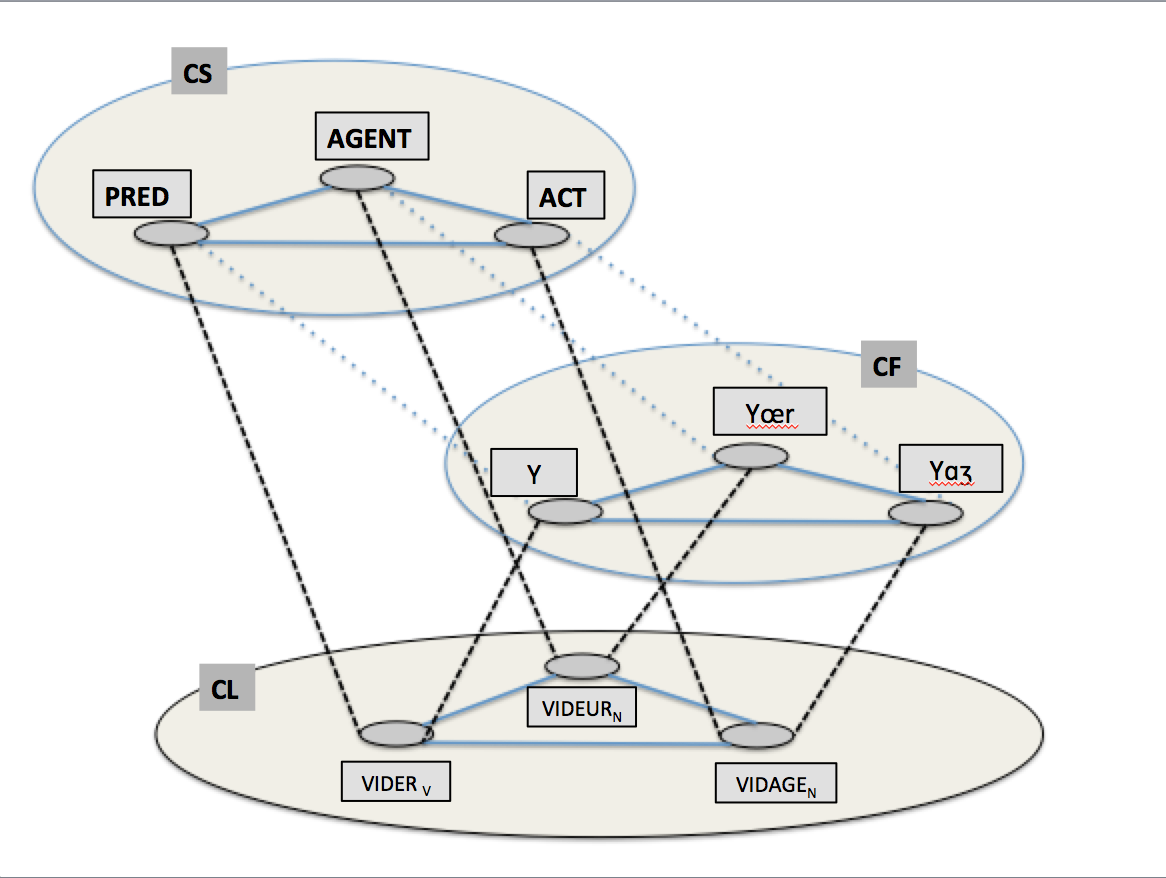
\includegraphics[width=0.8\linewidth]{figures/HatoutNamermodule-regulier.png}}
%  \fbox{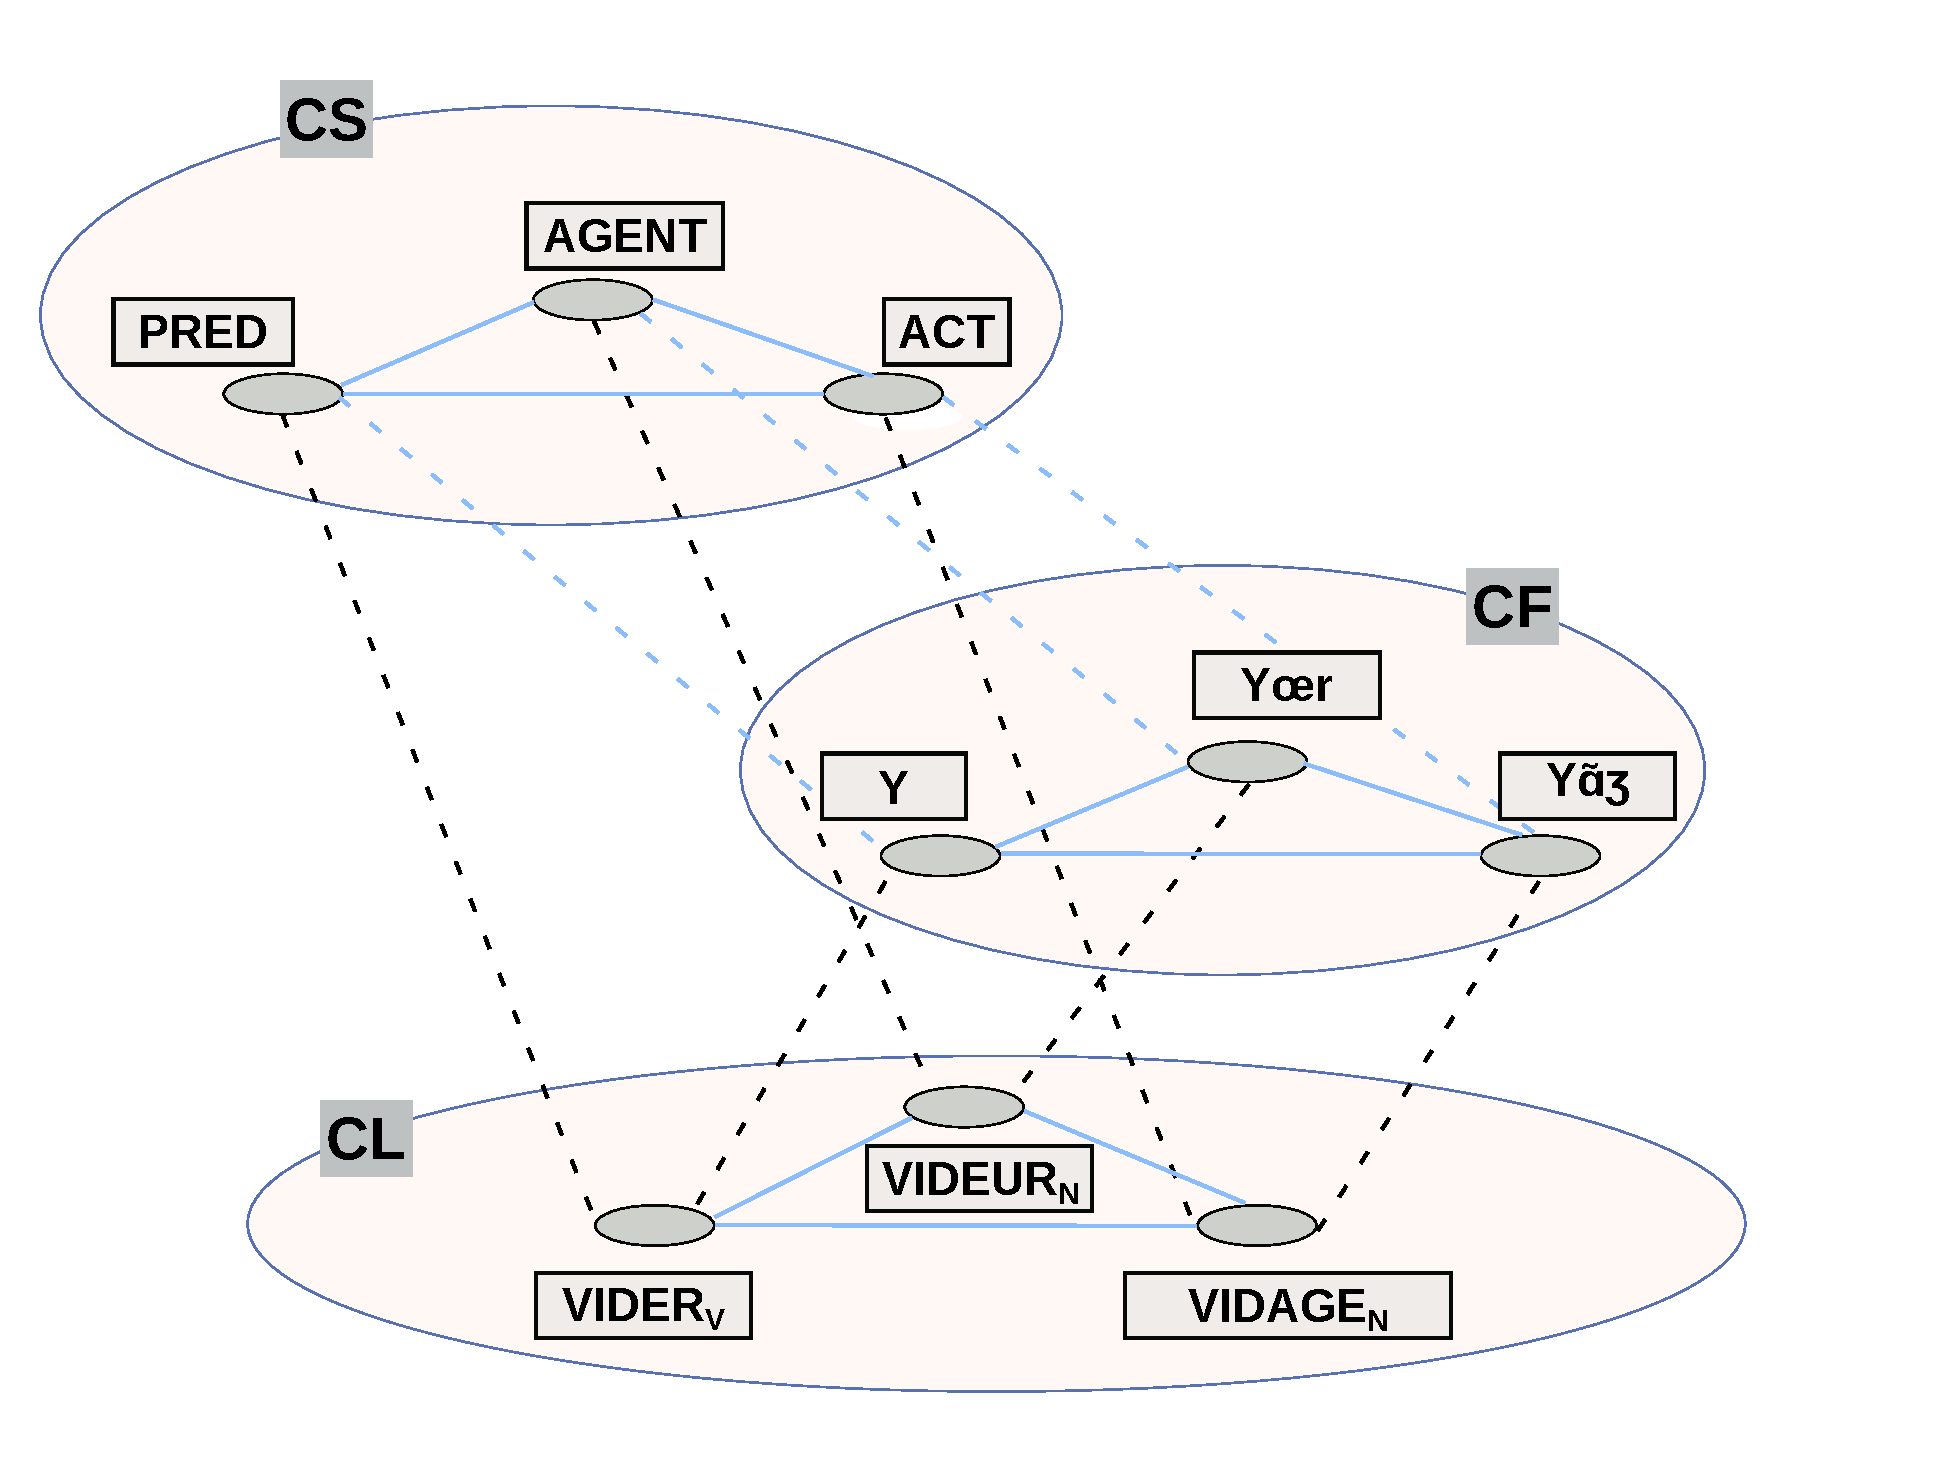
\includegraphics[width=0.8\linewidth]{figures/hathoutnamer-regulier.pdf}}
 \fbox{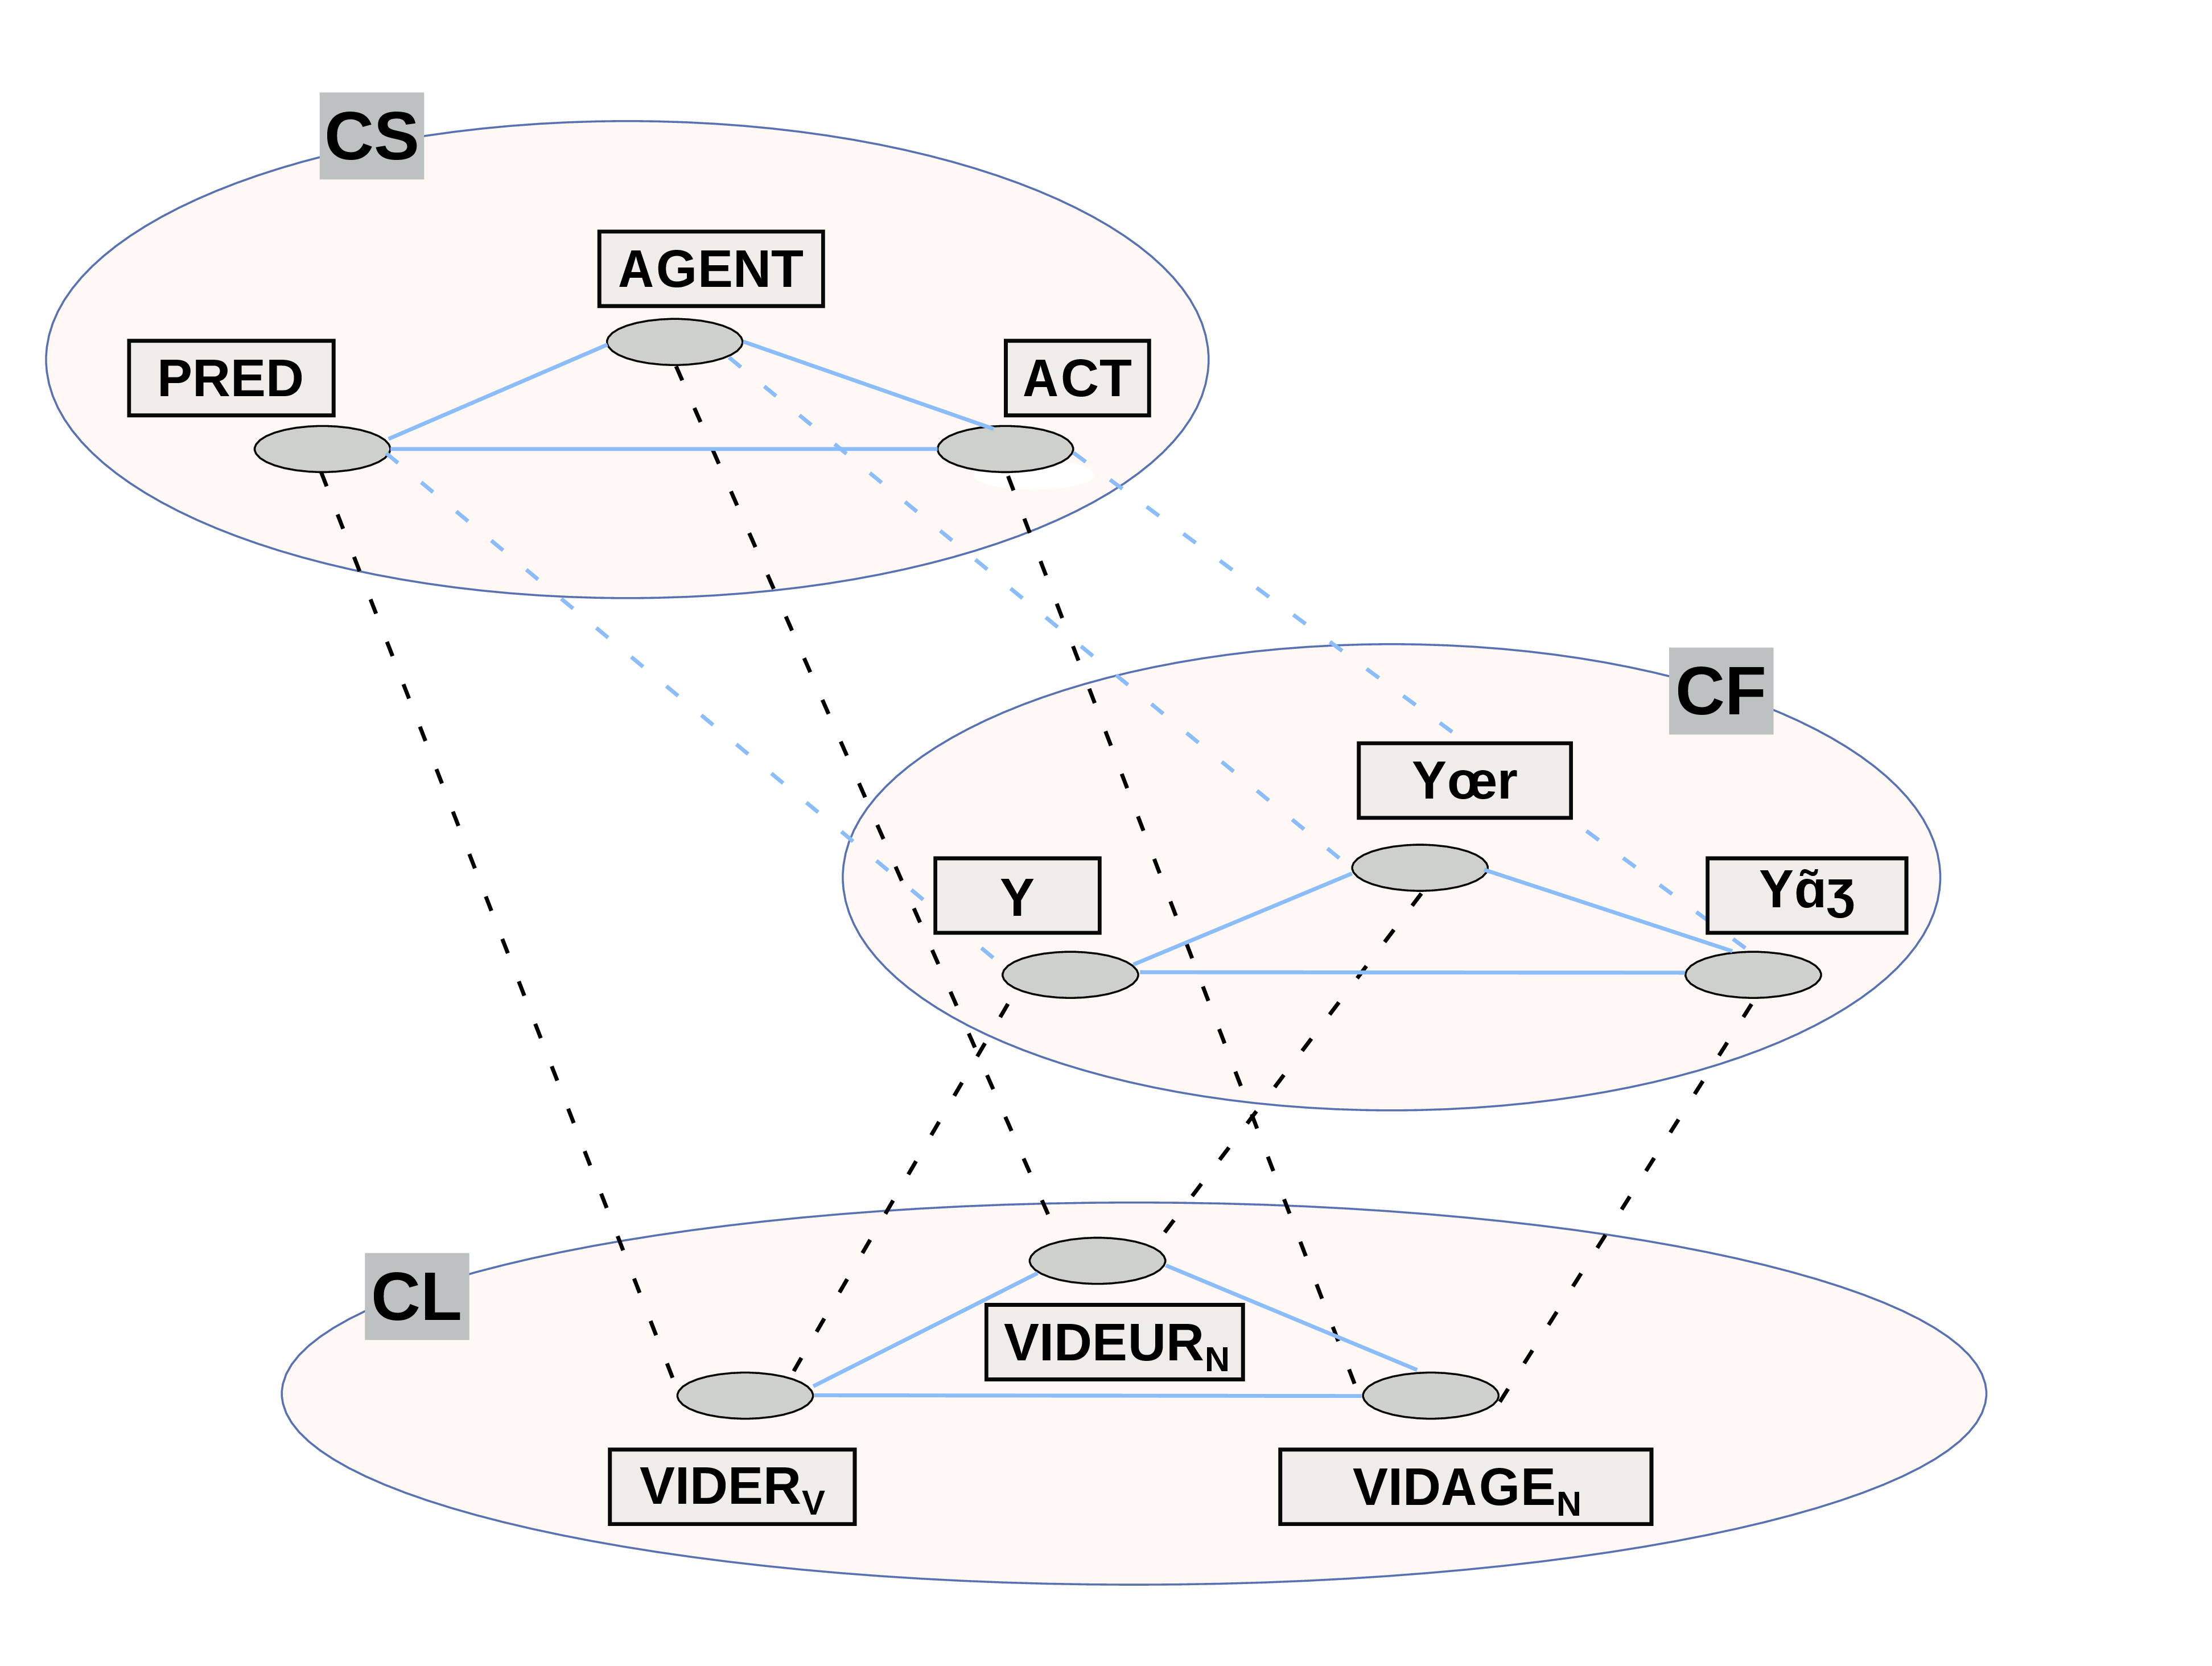
\includegraphics[width=0.8\linewidth]{figures/hathoutnamer-regulier.png}}
  \caption{Module correspondant à l'analyse de (\textsc{vider}, \textsc{videur}, \textsc{vidage}).  Le niveau catégoriel est omis.}
  \label{fig:module-regulier}
\end{figure}
%
La figure~\ref{fig:module-regulier} rend compte de la régularité paradigmatique\is{paradigm!derivational paradigm} qui caractérise le triplet (\textsc{vider}, \textsc{videur}, \textsc{vidage}), qui se manifeste dans la géométrie isomorphe\is{ParaDis model!isomorphy between components} (ici, triangulaire) des structures qui réalisent les composants formel (CF)\is{ParaDis model!formal component}, sémantique (CS)\is{ParaDis model!semantic component} et lexical (CL)\is{ParaDis model!lexical component}.

Pour alléger les graphiques des figures~\ref{fig:module-regulier} à~\ref{fig:antimilitariste}, le composant catégoriel\is{ParaDis model!categorial component} n'est pas représenté explicitement.  Nous avons indiqué sous forme d'indices dans le composant lexical\is{ParaDis model!lexical component} les catégories grammaticales auxquelles appartiennent les lexèmes\is{lexeme} connectés.  Les lignes continues représentent les connexions entre les éléments au sein d'un composant\is{ParaDis model!component}, et les lignes en pointillé relient les composants entre eux.  La régularité de la construction de (\textsc{vider}, \textsc{videur}, \textsc{vidage}) se traduit par une connexion doublement motivée dans le CL\is{ParaDis model!lexical component} entre les éléments du triplet. Chacune de trois relations concrètes dans le CL\is{ParaDis model!lexical component} est en effet l'instance de la relation abstraite correspondante dans les deux autres composants\is{ParaDis model!component}.

\subsection{L'analyse «~\textsf{ParaDisiaque}~» des adjectifs en \emph{\mbox{anti-$X$-suf}}}
\label{sec:analyse-anti}


% \subsubsection{ Les adjectifs préfixés en \emph{\mbox{anti-}}}
% \label{sec:adjectifs-prefixes-anti}

%\textcolor{red}{dire deux mots de la distinction abstr/conc pour les paradigmes}

%Fradin 2003 n'inclut pas les préfixés adjectivaux parmi les constructions dites parasynthétiques. Parmi ceux-ci, souvent qualifiés de cas de "bracketing paradox"(Pesetzky 19851, Williams 19812, see also e.g. Becker 1993, XXX), nous nous intéressons aux adjectifs adversatifs, i.e. qui s'interprètent `qui s'oppose à @' où @ réfère à une entité (Hathout 2011, XXX).


Nous avons montré que  la dérivation parasynthétique était un modèle de préfixation\is{prefixation} répandu dans les langues, fréquemment observable pour une grande variété de suffixes\is{suffixation}, et, comme a pu le montrer \cite{hathout2011.dumal}, extrêmement productif.  Pour un dérivé \emph{\mbox{pref-$X$-suf}},  la marque suffixale \emph{suf} coïncide avec l'exposant de l'un des dérivés suffixés\is{suffixation} de $X$, i.e.\ \emph{\mbox{$X$-suf}} quand celui-ci est attesté, témoignant ainsi du fait que, si \emph{\mbox{pref-$X$-suf}} se définit par rapport à $X$, sa forme emprunte
 le segment \emph{suf} au lexème\is{lexeme} \emph{\mbox{$X$-suf}} dérivationnellement apparenté à $X$.  La modélisation du schéma de construction de ces formes doit donc inclure un dispositif d'accès aux membres de la famille\is{derivation!derivational family} de $X$. En nous servant de l'analyse de l'adjectif \textsc{antimilitariste}, voyons comment ce mécanisme est réalisé dans \paradis{}\is{ParaDis model}.

% \subsubsection{Analyse d'\textsc{antimilitariste}}
% \label{sec:analyse-antimilitariste}

La représentation d'\textsc{antimilitariste}, dans la figure~\ref{fig:antimilitariste1}, se distribue suivant quatre dimensions\is{ParaDis model!four representation levels}~: c'est un adjectif~; il instancie la classe conceptuelle d'opposition comme l'indique l'étiquette {CONTRE} dans le CS\is{ParaDis model!semantic component}~; il vérifie le patron formel $\textrm{ɑ̃ti}X\textrm{ist}$
 dans le CF\is{ParaDis model!formal component}.  Le module\is{ParaDis model!module} d'\textsc{antimilitariste}
%M\indi{\textsc{antimilitariste}},
inclut dans son CL\is{ParaDis model!lexical component} le nom \textsc{militaire} avec lequel \textsc{antimilitariste} entretient une relation sémantiquement motivée~: «~une chanson antimilitariste~» est `une chanson contre les militaires', et plus généralement `une chanson contre l'armée'.  La connexion entre les deux lexèmes\is{lexeme} est donc héritée du composant sémantique\is{ParaDis model!semantic component} où le concept {CONTRE} requiert nécessairement l'existence d'une entité ({ENTITÉ}) qui est l'objet de cette opposition. Cette relation est régulière~: toute entité (concrète ou abstraite) peut déclencher une réaction d'opposition, et à toute attitude hostile correspond nécessairement l'objet rejeté.

En revanche, il n'existe pas de justification formelle à cette relation~: \textsc{militaire} dont la forme est une instance du patron $Y\textrm{ɛʁ}$ 
 (en considérant \emph{militaire} comme formé sur le thème supplétif\is{stem!suppletive} \textsuperscript{o}/milit/
  de \textsc{armée}), ne permet pas la prédiction de~$\textrm{ɑ̃ti}X\textrm{ist}$, et réciproquement. Il apparaît ainsi un décalage entre la régularité sémantique et l'absence de lien formel entre \textsc{antimilitariste} et \textsc{militaire}, ce qu'illustre la figure~\ref{fig:antimilitariste1}~: la ligne continue qui connecte {CONTRE} et {ENTITÉ} dans le CS\is{ParaDis model!semantic component} n'a pas de correspondant dans le CF\is{ParaDis model!formal component}. La motivation sémantique justifie donc seule la relation qui unit, dans le CL\is{ParaDis model!lexical component}, \textsc{antimilitariste} et \textsc{militaire}.
%
\begin{figure}
  \centering
%   \fbox{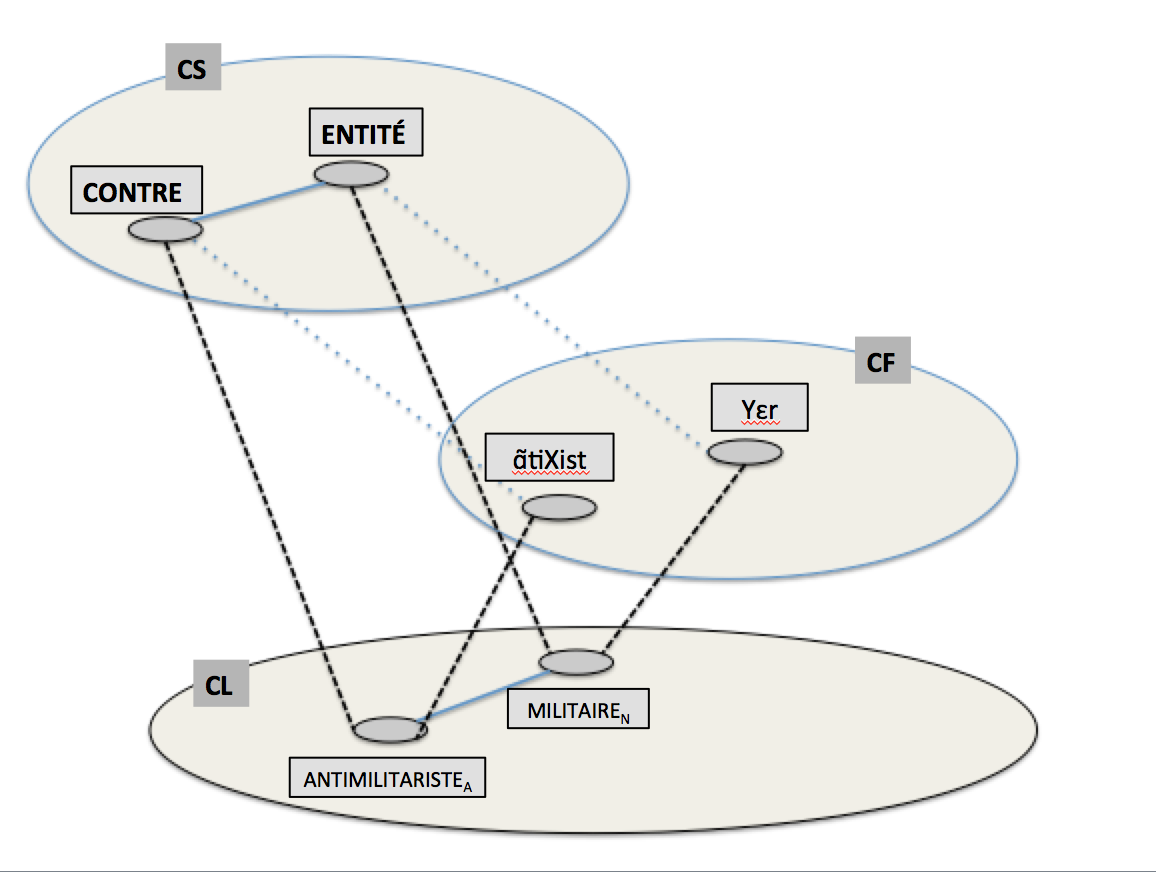
\includegraphics[width=0.8\linewidth]{figures/HatoutNamermodule-antimilitariste1.png}}
%   \fbox{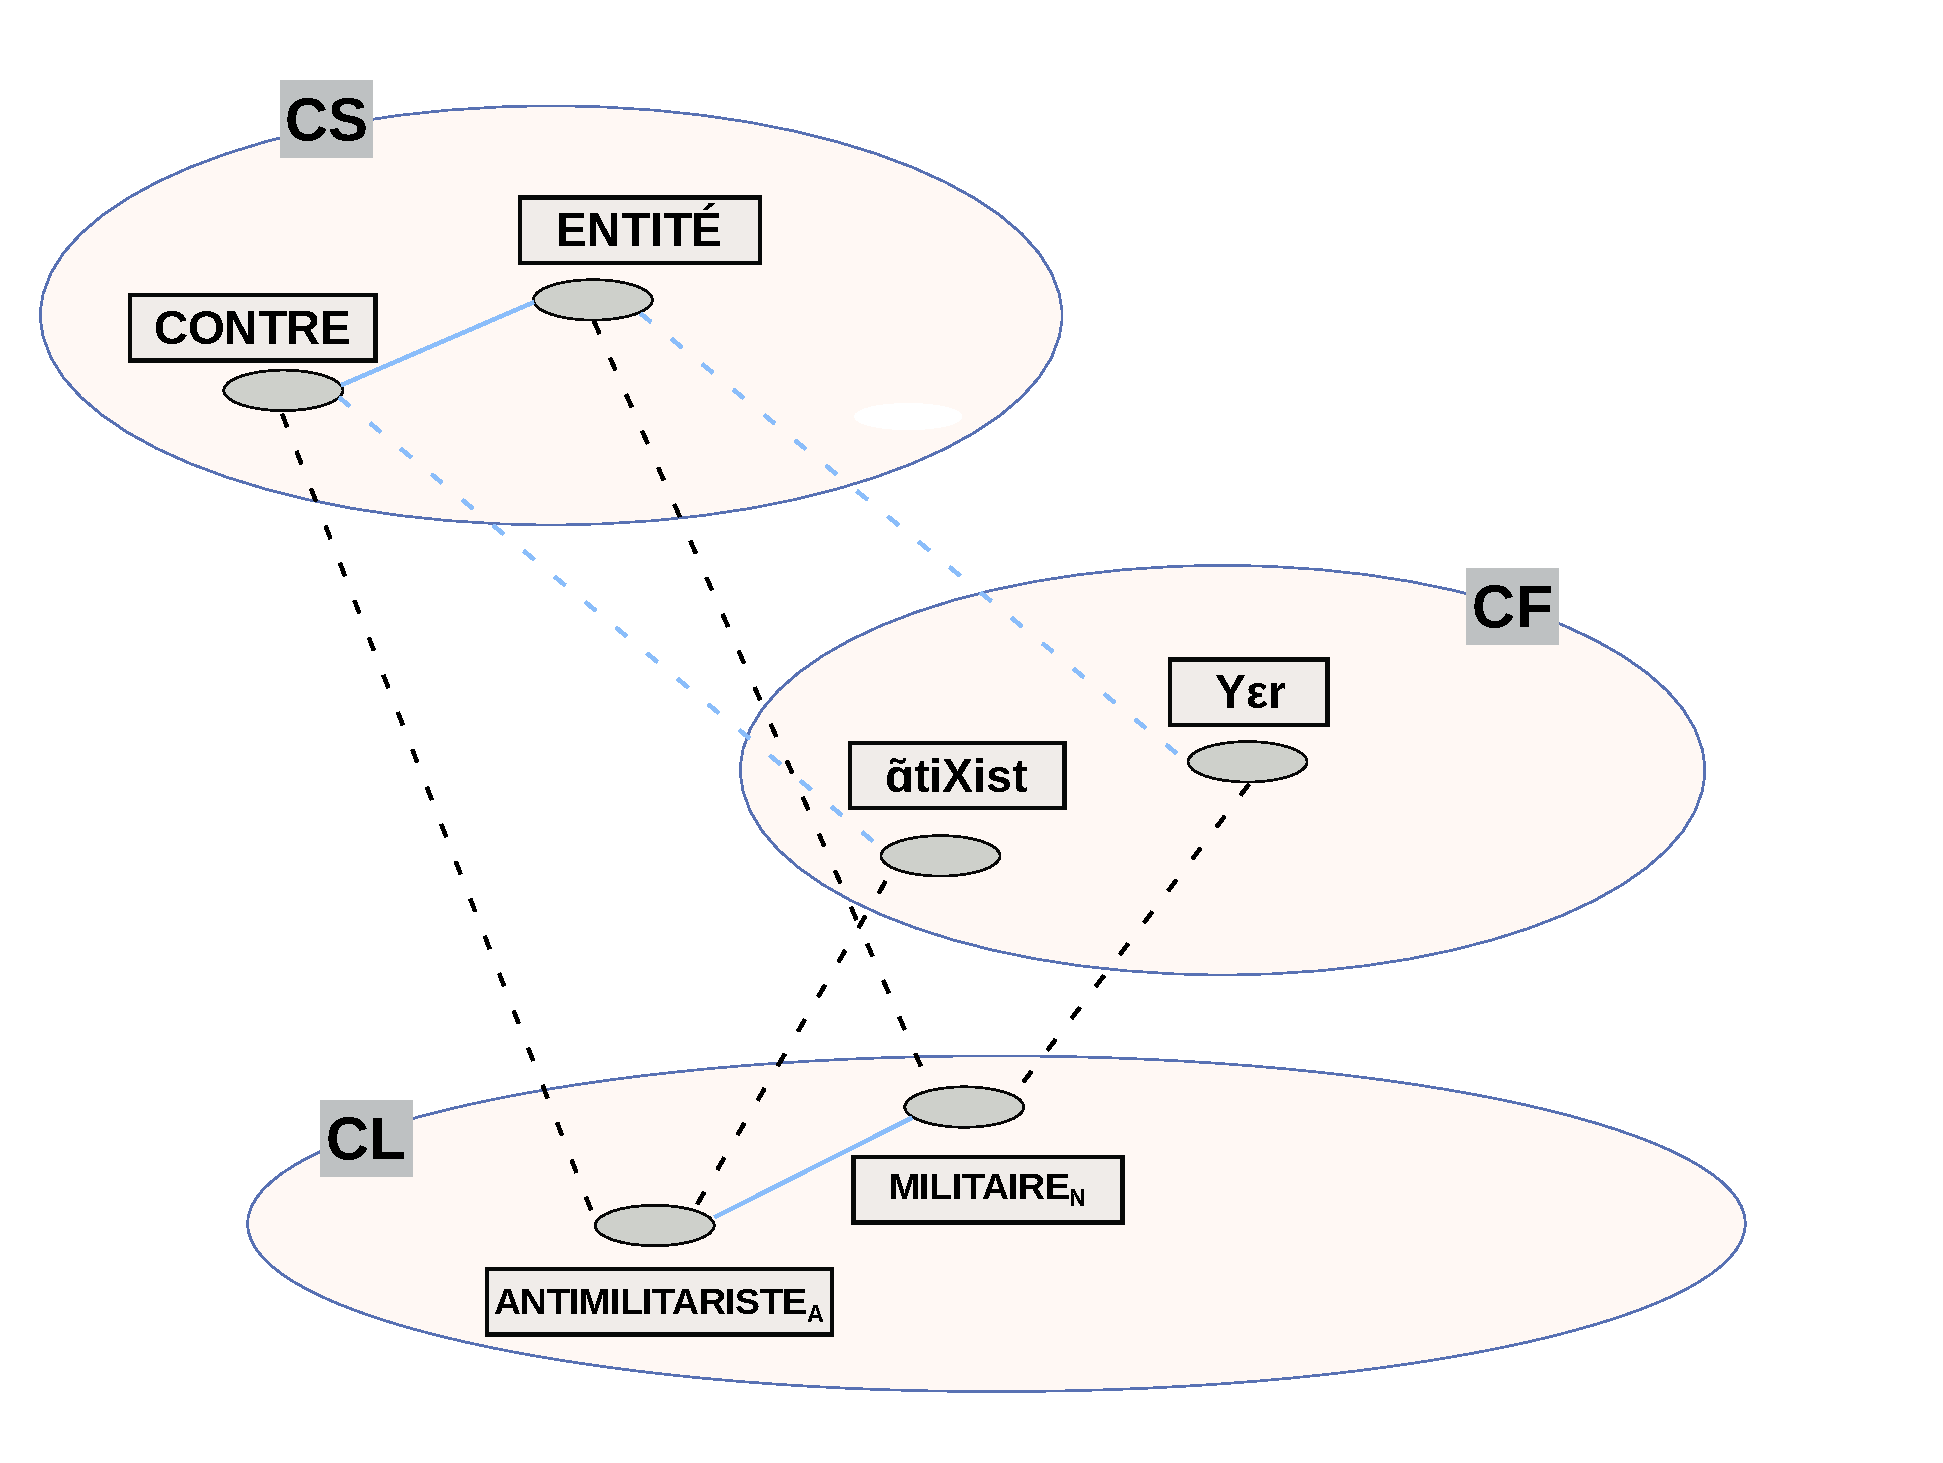
\includegraphics[width=0.8\linewidth]{figures/hathoutnamer-anti1.pdf}}
  \fbox{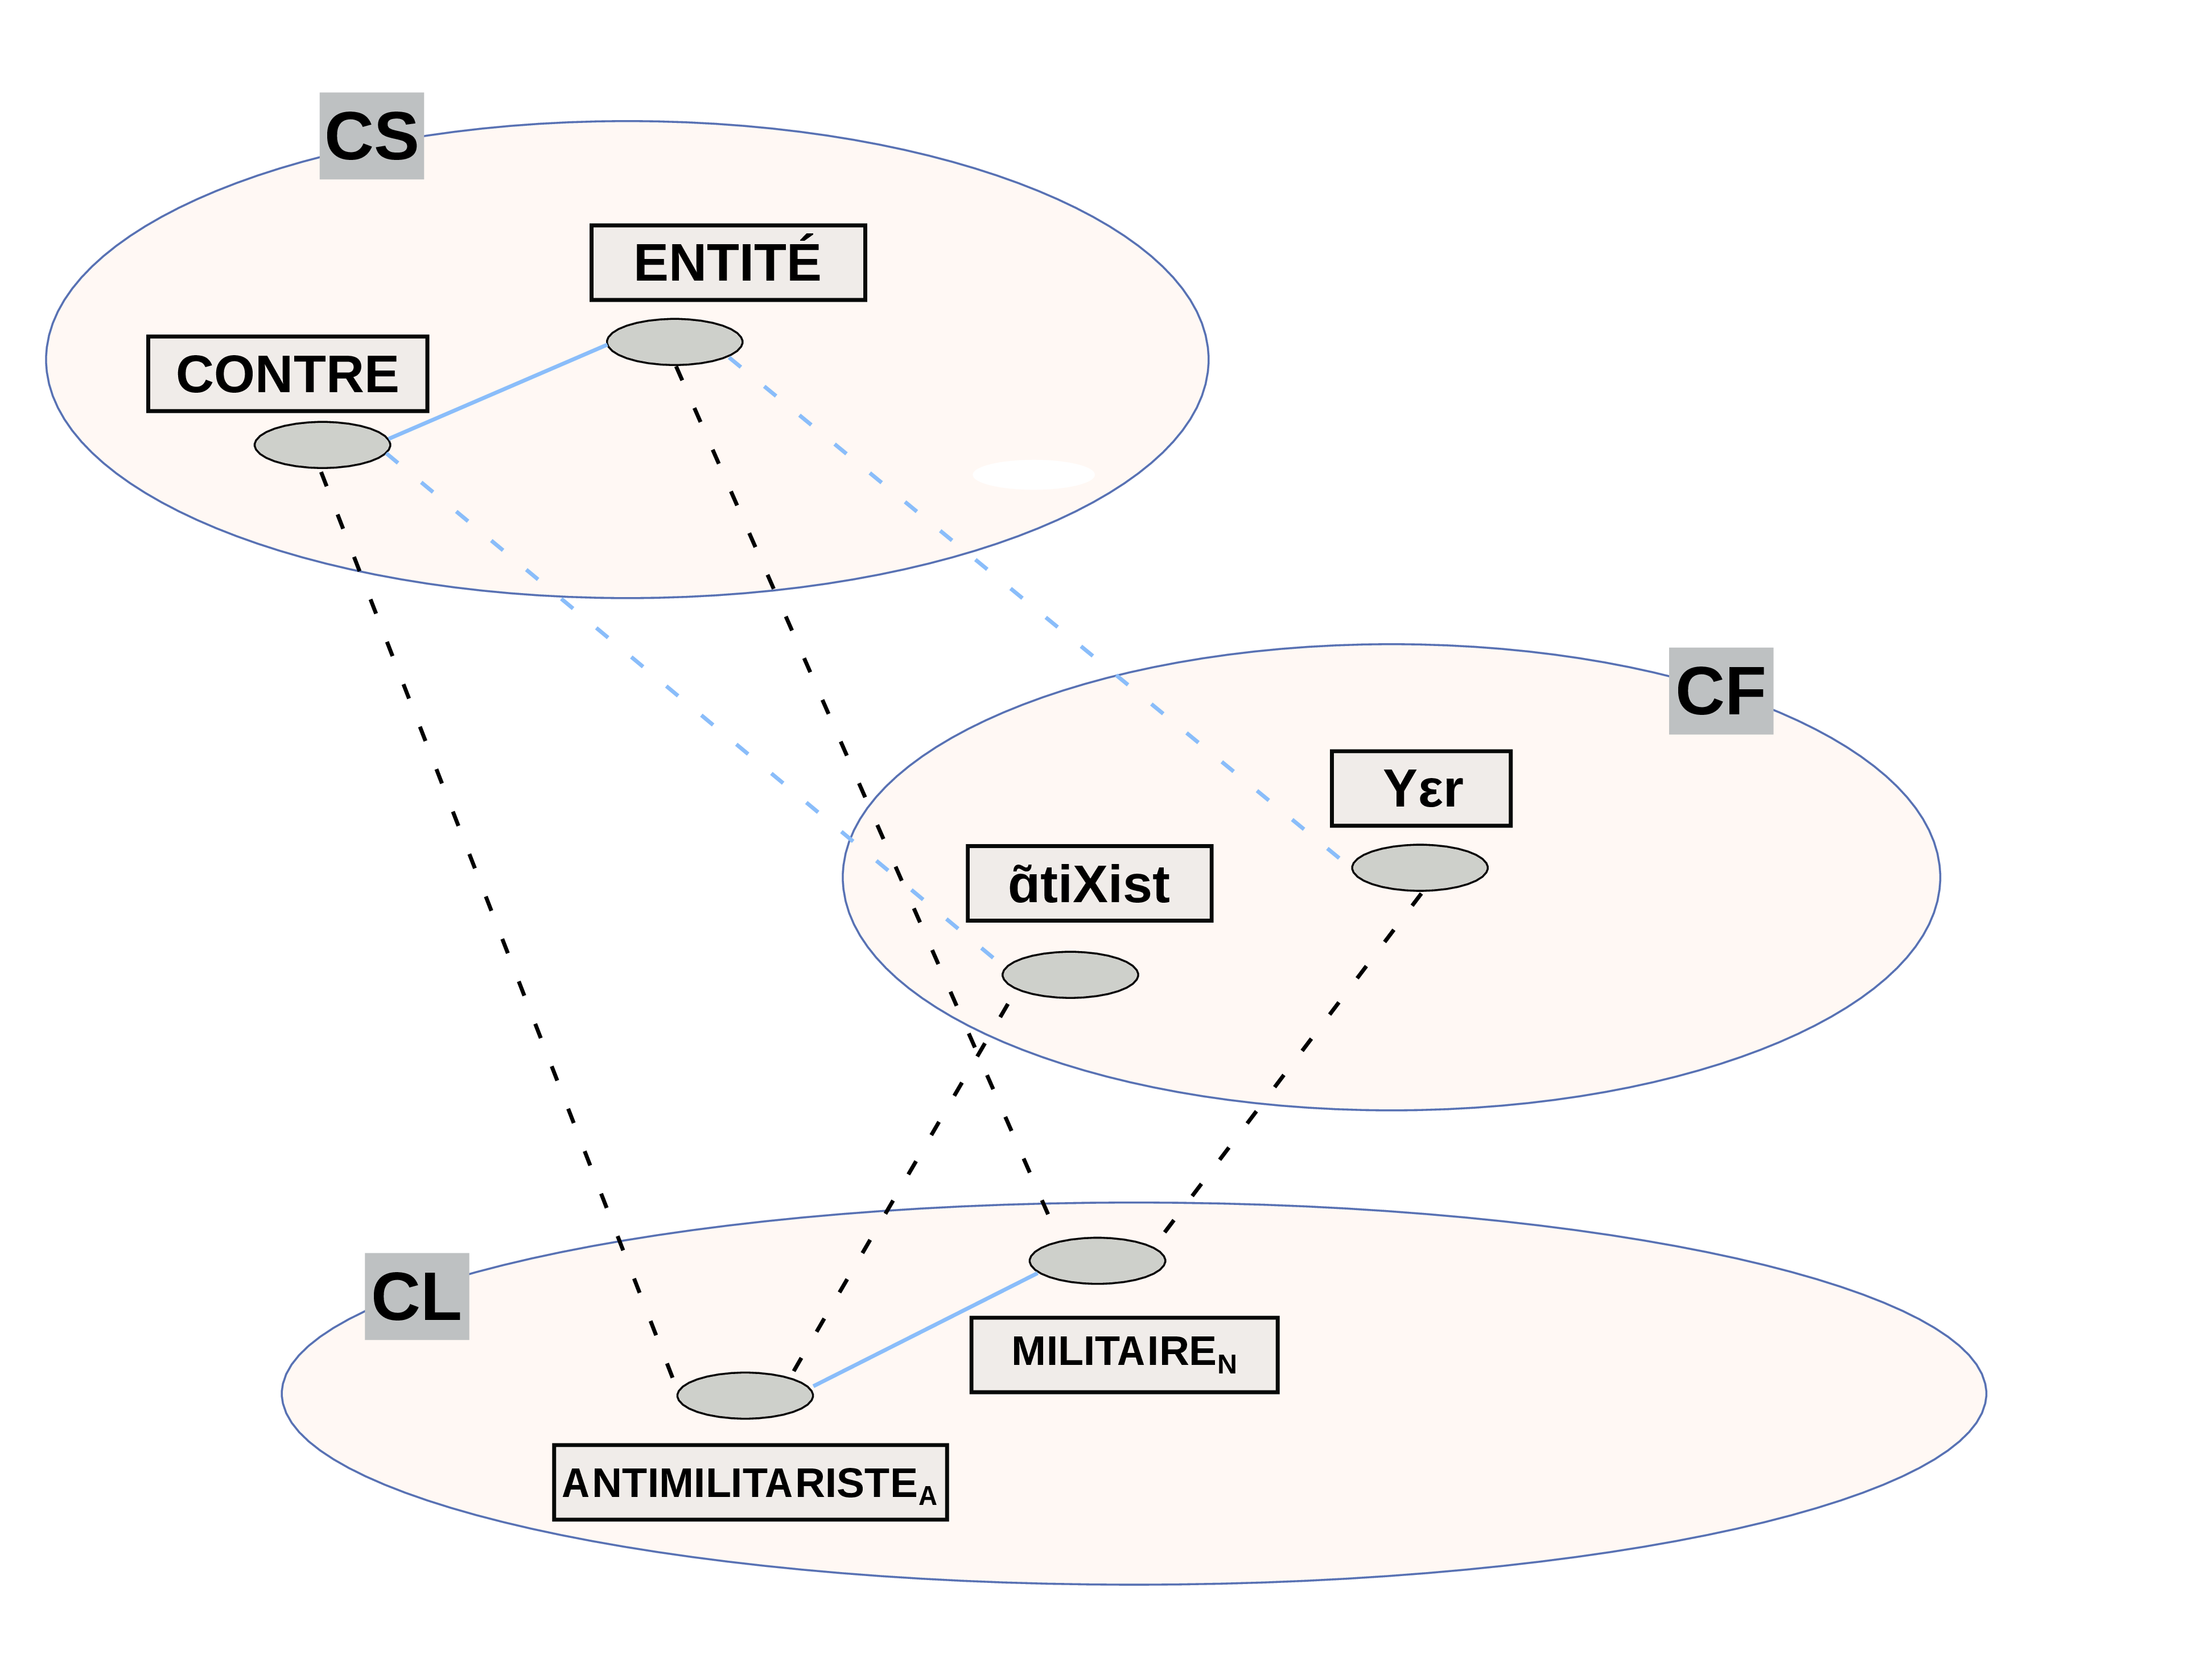
\includegraphics[width=0.8\linewidth]{figures/hathoutnamer-anti1.png}}
  \caption{Élément de l'analyse de \textsc{antimilitariste}~: la motivation sémantique \textsc{antimilitariste} $\leftarrow$  \textsc{militaire}}
  \label{fig:antimilitariste1}
\end{figure}

Puisque la forme de \textsc{antimilitariste} ne coïncide pas avec sa construction sémantique, c'est dans le voisinage dérivationnel de l'adjectif que l'on va chercher la motivation\is{derivation!motivation} de sa structure morphologique. Le nom (et adjectif) \textsc{militariste} répond à cette exigence.  En effet, formellement, \textsc{militariste} est une instance du patron $X$ist% was:\textipa{ist}
, et entretient une relation d'interprédictibilité avec \textsc{antimilitariste}, \emph{\mbox{anti-}} apparaissant fréquemment dans des structures comportant une finale en /ist/% was:\textipa{/ist/}
\footnote{%
  Dans TLFindex par exemple, 11\% des adjectifs de la forme $\textrm{ɑ̃ti}X$ finissent en \emph{\mbox{-iste}} (i.e.\ sont des instances de $\textrm{ɑ̃ti}X\textrm{ist}$).%
}.  C'est ce qui est représenté dans la figure~\ref{fig:antimilitariste2}.   En revanche, la relation entre \textsc{antimilitariste} et \textsc{militariste} ne répond à aucune motivation sémantique comme l'indique l'absence  de relation d'interprédictibilité entre les catégories sémantiques {CONTRE} et {PARTISAN} dans la figure~\ref{fig:antimilitariste2}~: en l'occurrence, l'émergence d'un comportement adversatif ({CONTRE}) ne requiert pas l'existence d'un {PARTISAN}.
%
\begin{figure}
  \centering
  \fbox{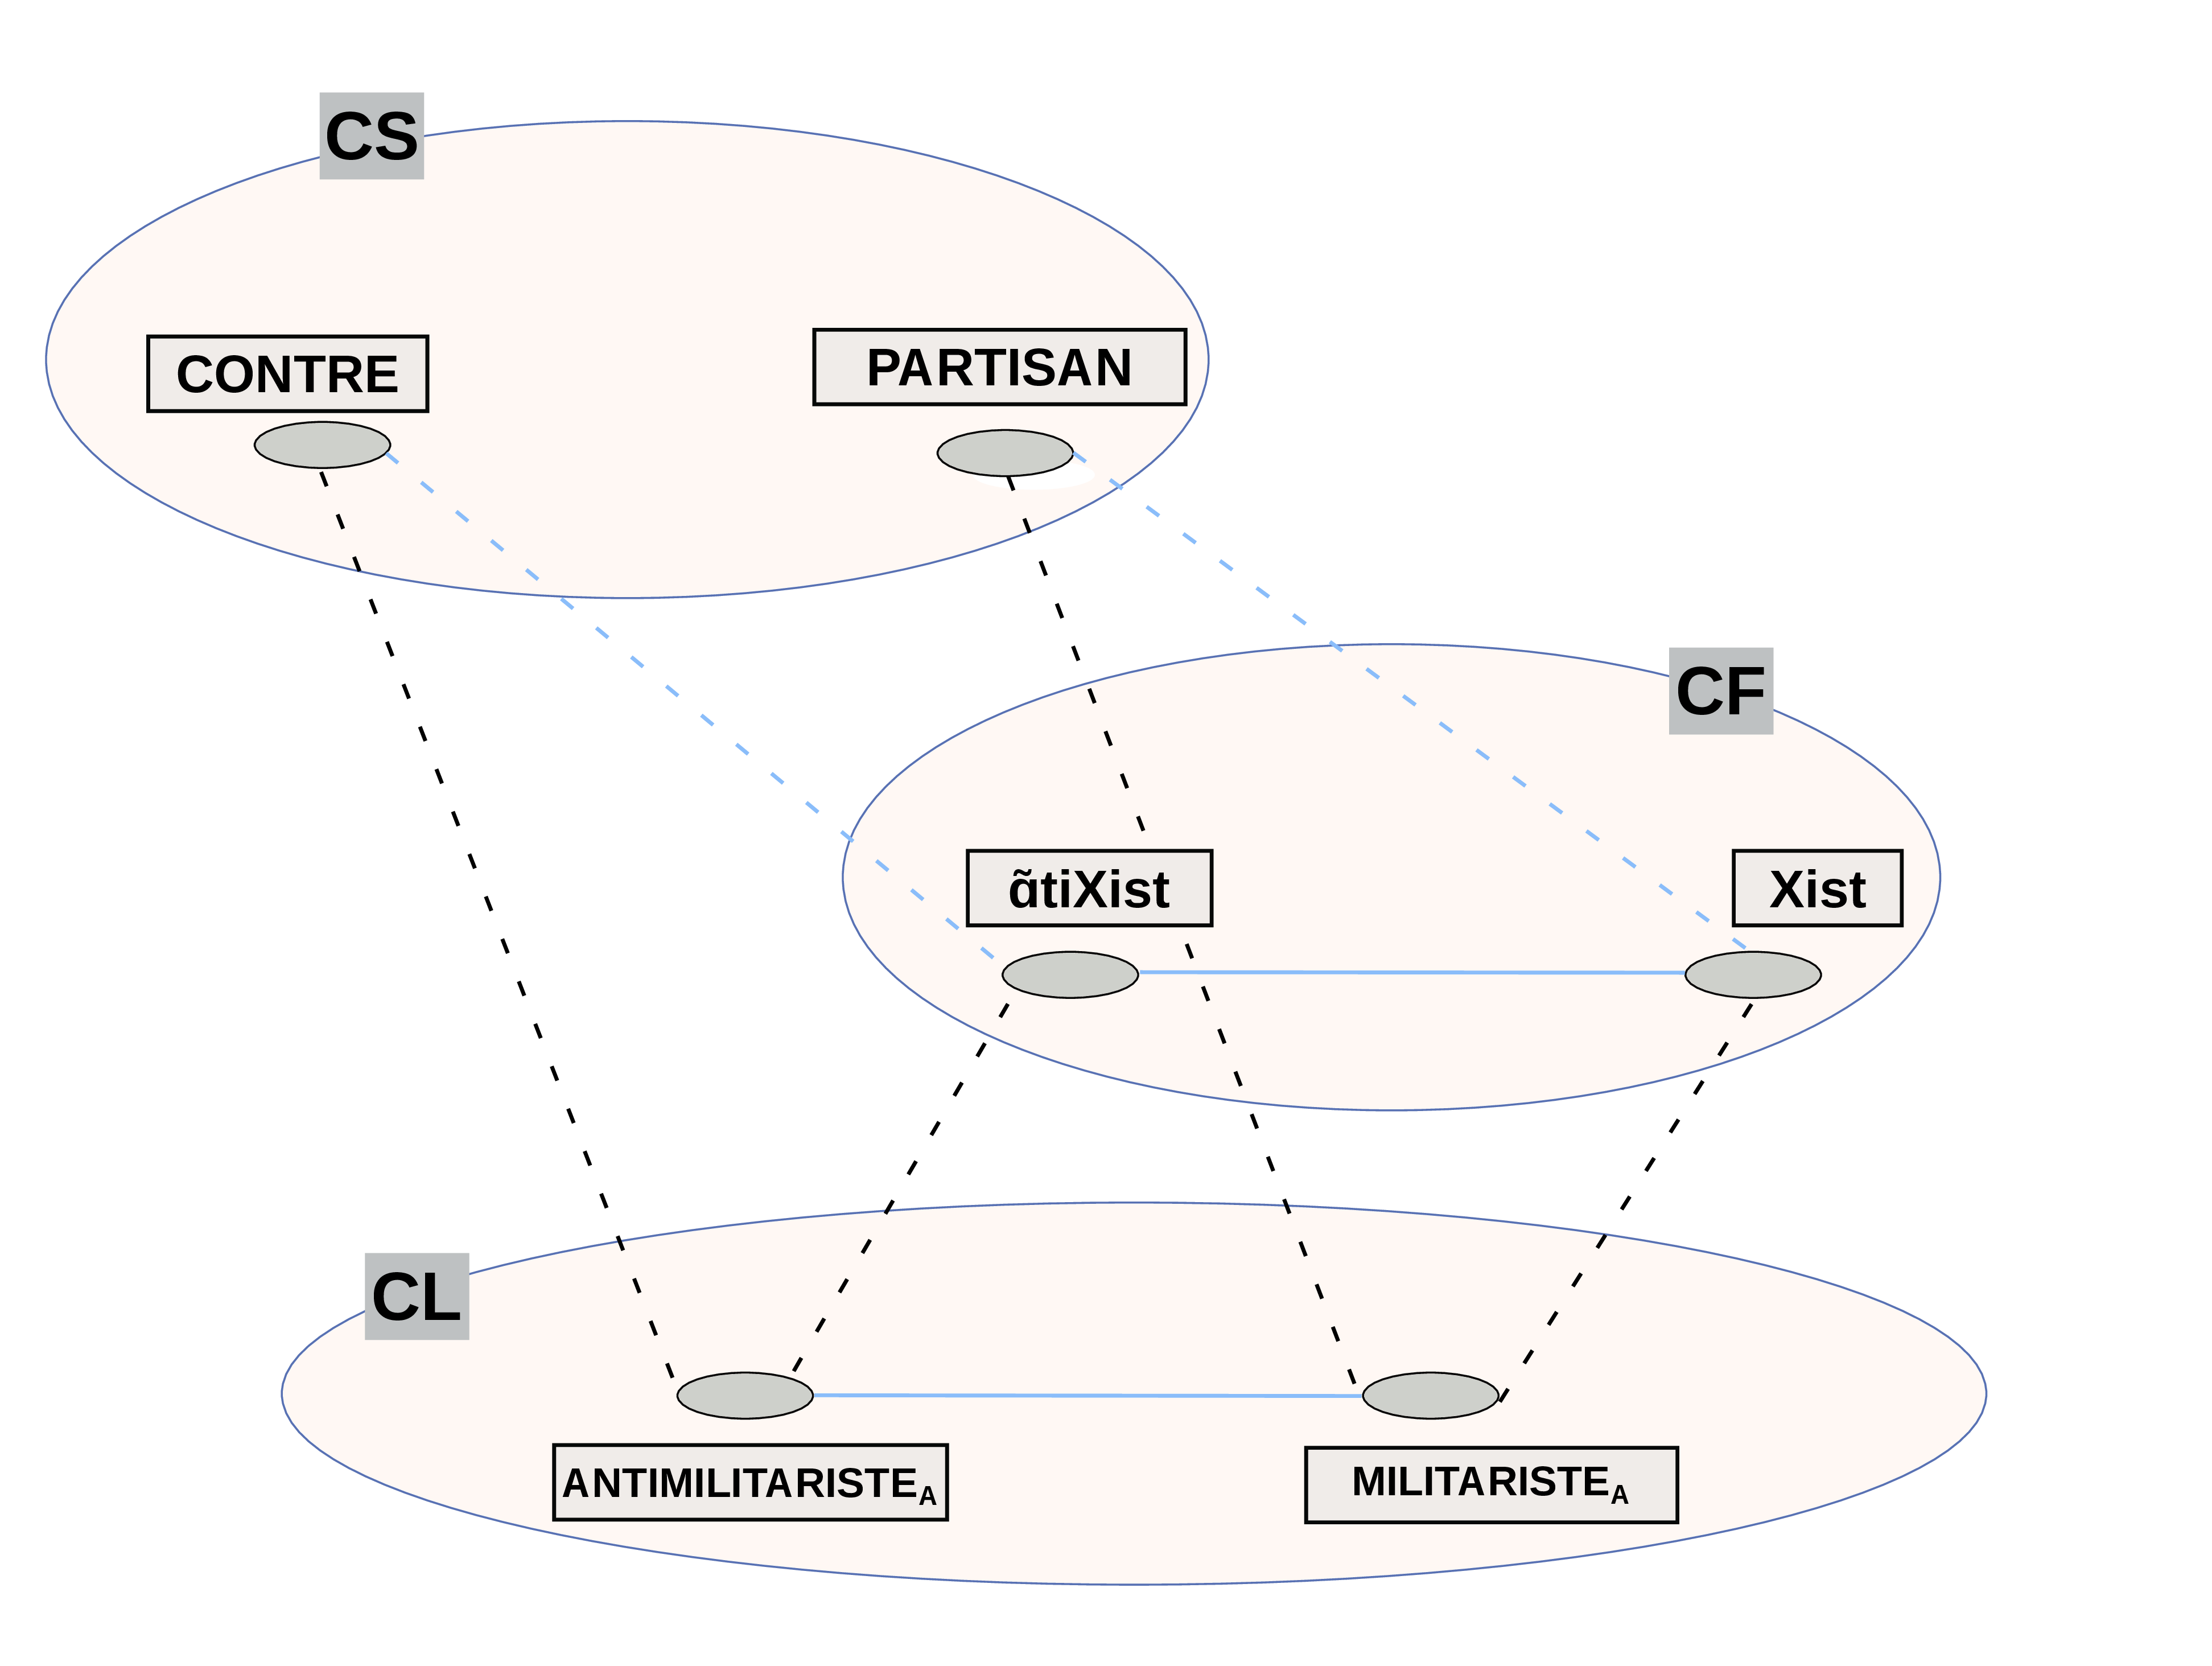
\includegraphics[width=0.8\linewidth]{figures/hathoutnamer-anti2.png}}
% 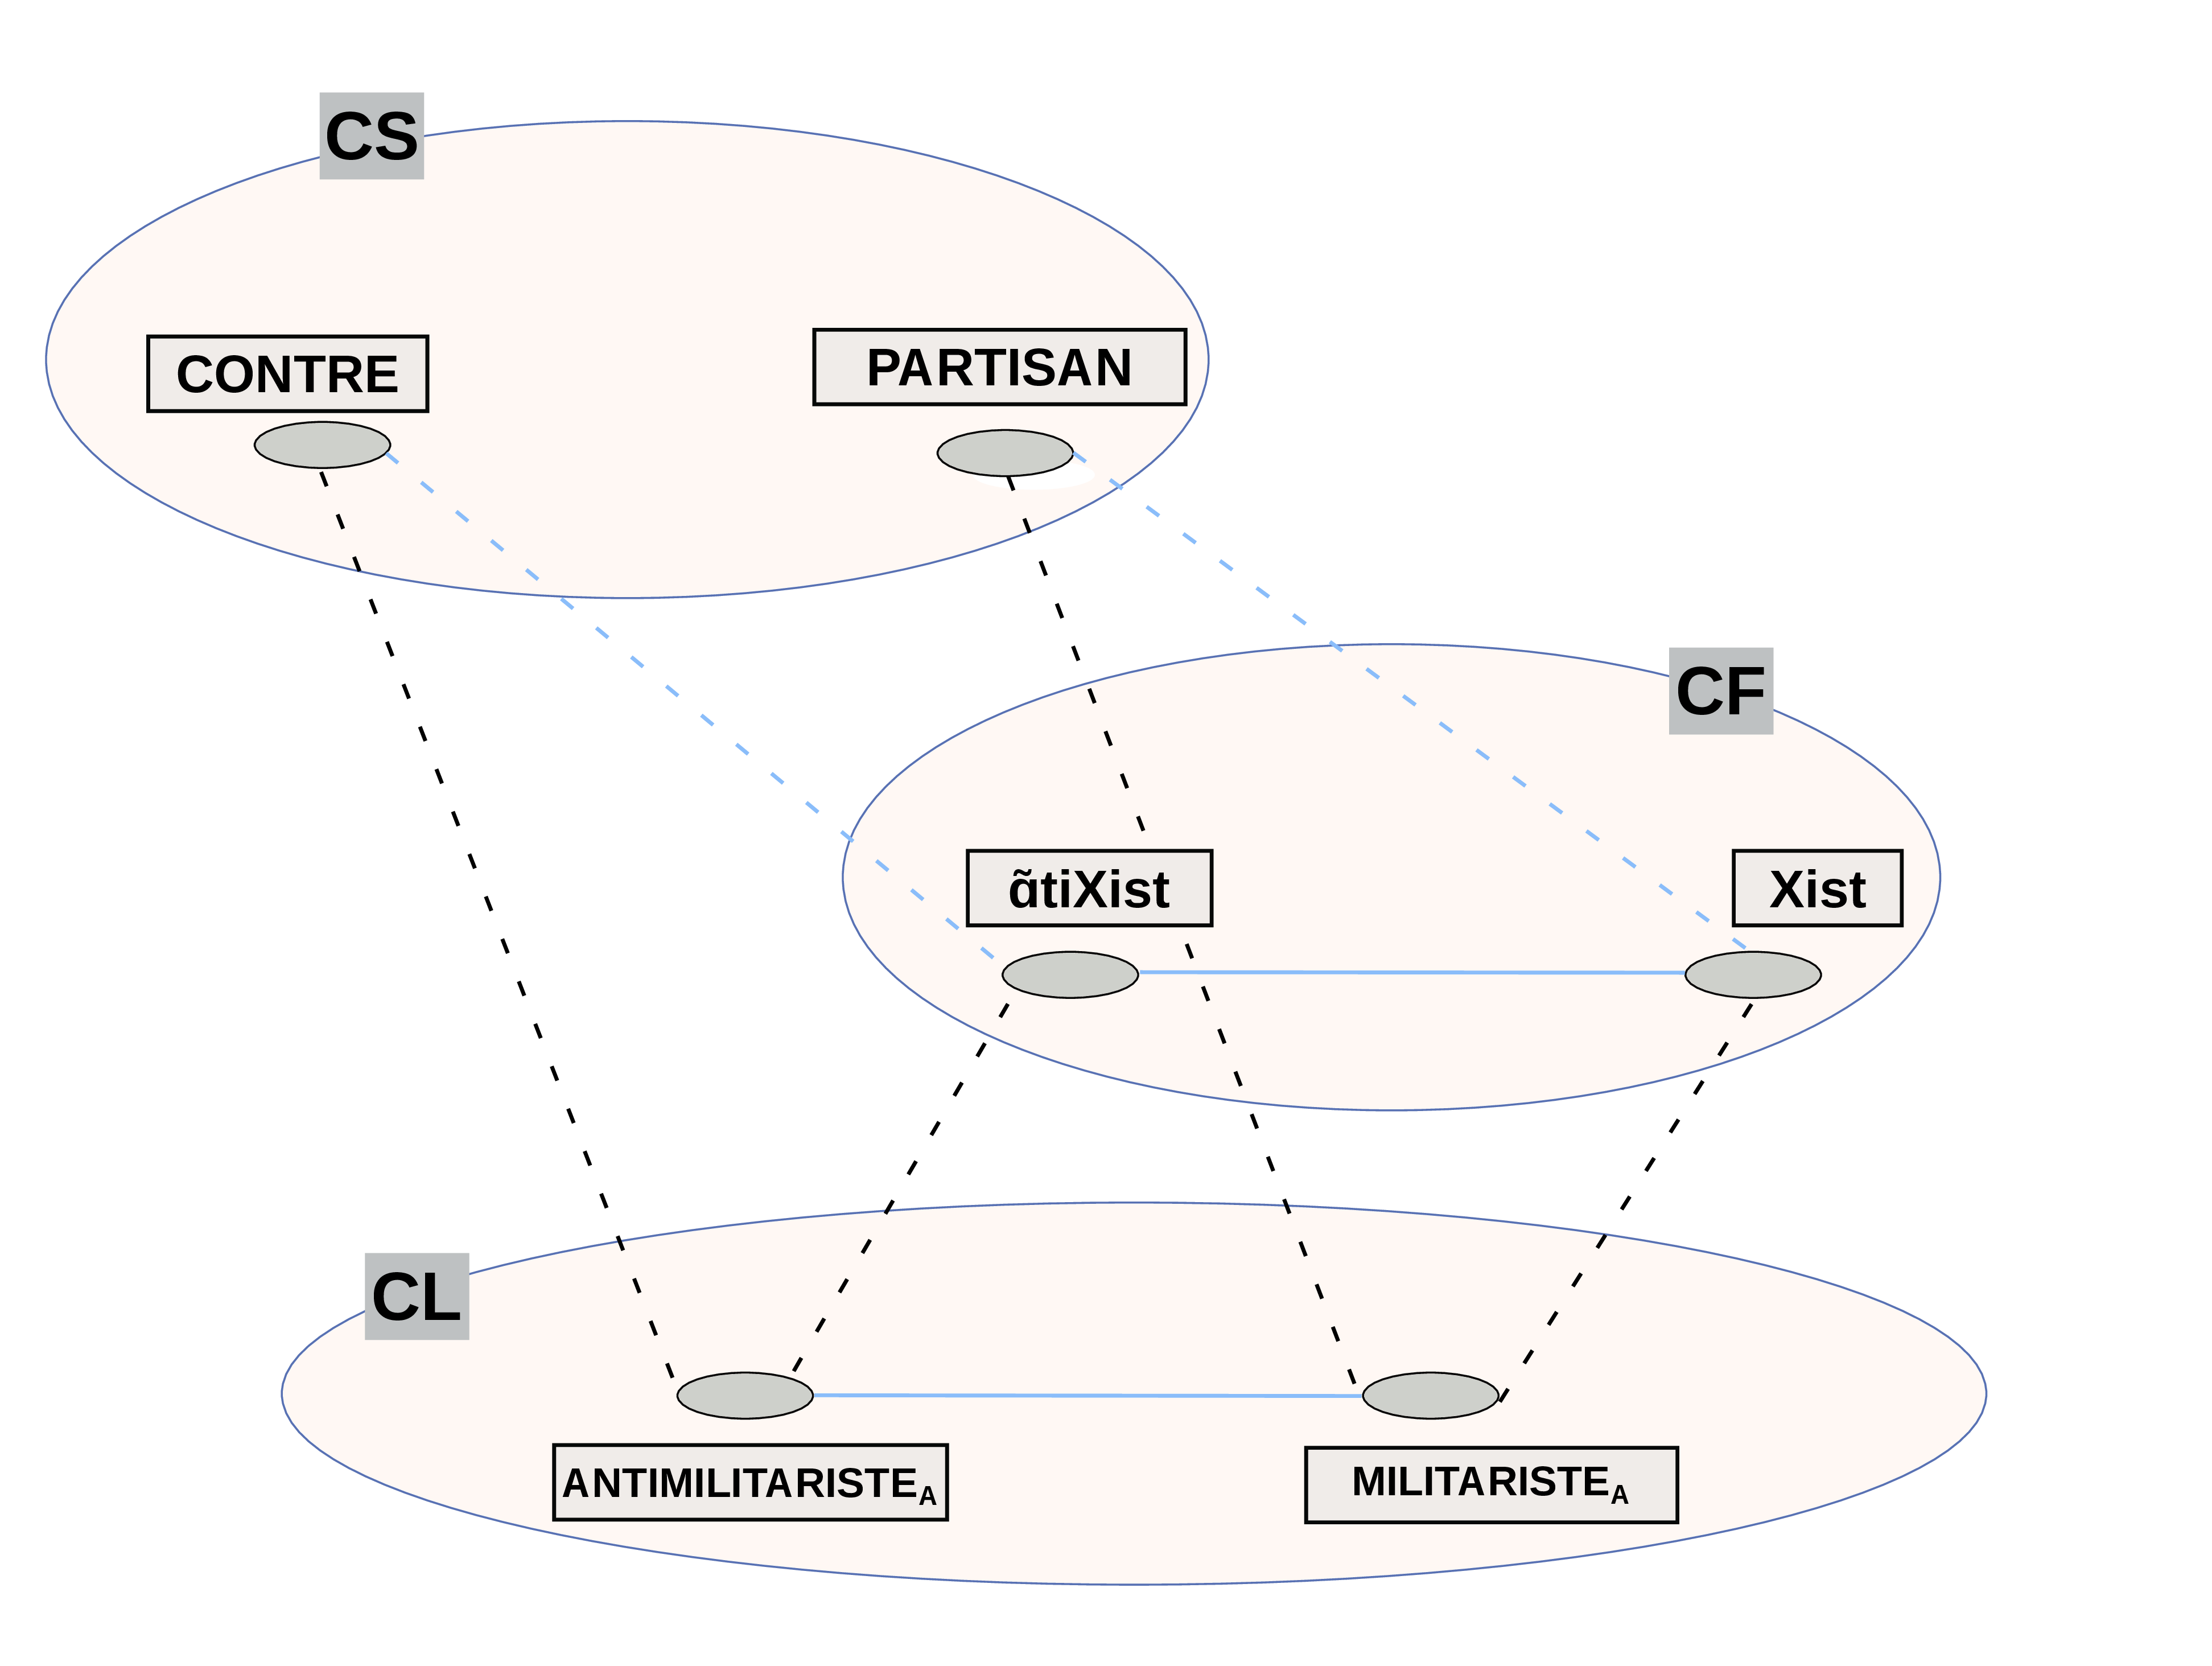
\includegraphics[width=0.8\linewidth]{figures/hathoutnamer-anti2.png}}
%   \fbox{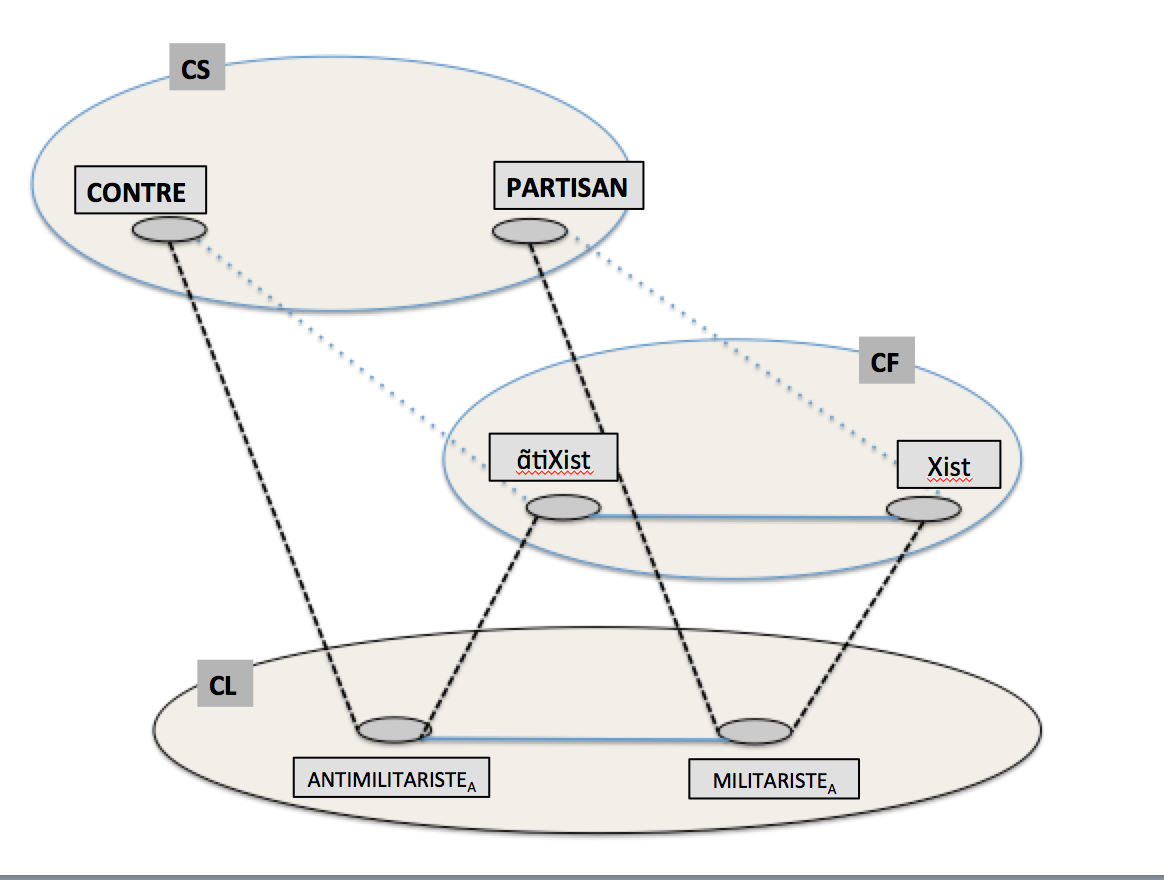
\includegraphics[width=0.8\linewidth]{figures/HatoutNamermodule-antimilitariste2.png}}
  \caption{Élément de l'analyse de \textsc{antimilitariste}~:  la motivation formelle \textsc{antimilitariste} $\leftarrow$  \textsc{militariste}}
  \label{fig:antimilitariste2}
\end{figure}

{PARTISAN}, la catégorie sémantique de \textsc{militariste}, est en contrepartie indissociable de celle de l'objet valorisé, qui peut être une idéologie (le \emph{pointillisme}, pour le \emph{pointilliste}), un individu (\emph{Sarkozy}, pour le \emph{Sarkoziste}), une fonction (le \emph{pape}, pour un \emph{papiste}), une activité (\emph{bouger}, pour le \emph{bougiste}), un objet concret (la \emph{viande}, pour le \emph{viandiste}), etc.  C'est en d'autres termes une entité conceptuelle non contrainte, que nous représentons par la classe {ENTITÉ} (voir \cite{roche2007.isme-decembrettes,roche2011.isme-dumal} pour une analyse détaillée des suffixations en \emph{\mbox{-isme}}\is{suffixation!in -\emph{isme}} et \emph{\mbox{-iste}}\is{suffixation!in -\emph{iste}} en français). La relation est également prédictible dans le CF\is{ParaDis model!formal component}~: la suffixation en \emph{\mbox{-iste}}\is{suffixation!in -\emph{iste}} présente une affinité notable avec les structures comportant une finale en /ɛʁ/% was:\textipa{/EK/}
\footnote{%
  Les noms et adjectifs en $X\textrm{aʁist}$ 
 forment 4\% des entrées en $Y\textrm{ist}$
 dans TLFindex.%
}. L'assemblage des quatre composants\is{ParaDis model!four representation levels}, illustré par la figure~\ref{fig:antimilitariste3}, montre que \textsc{militariste} forme avec \textsc{militaire} un module\is{ParaDis model!module}  sémantiquement et formellement régulier~: la géométrie dans les quatre composants est isomorphe\is{ParaDis model!isomorphy between components}.

\begin{figure}
  \centering
%   \fbox{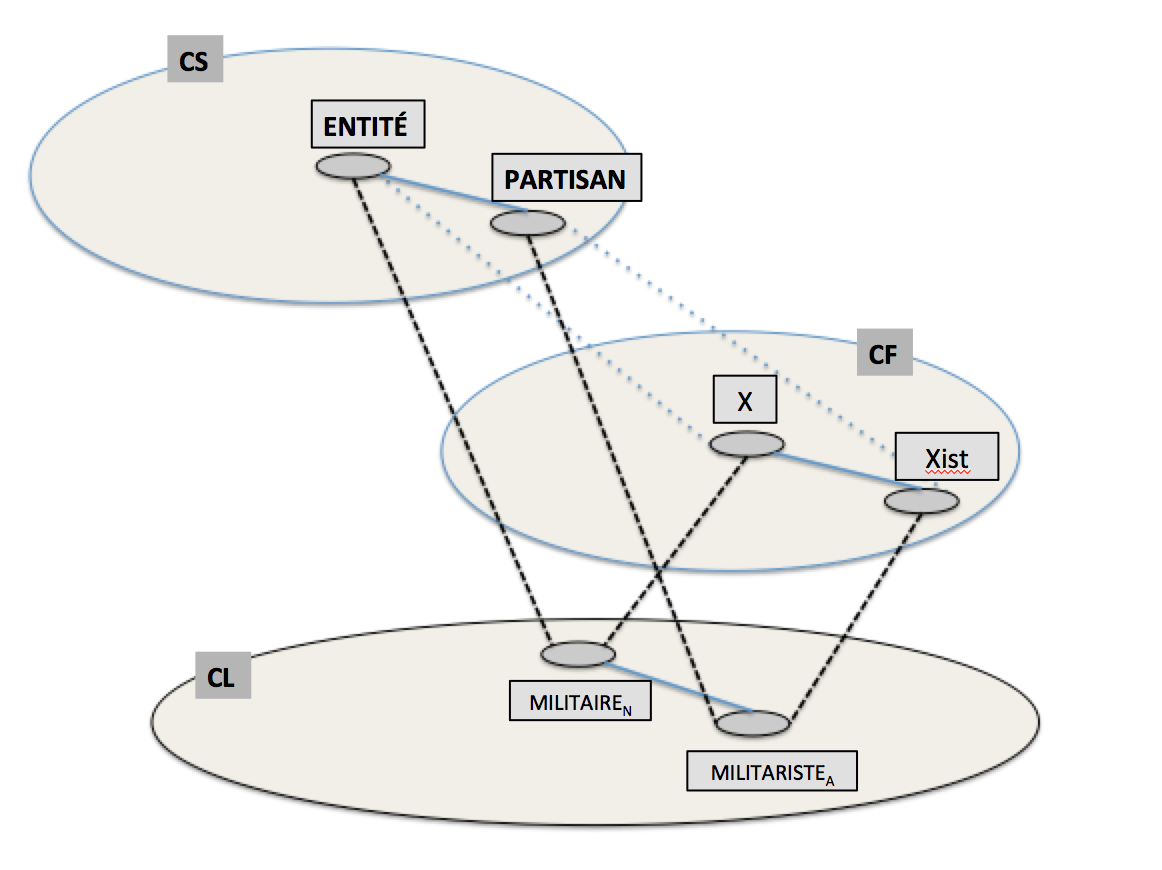
\includegraphics[width=0.8\linewidth]{figures/HatoutNamermodule-antimilitariste3.png}}
%   \fbox{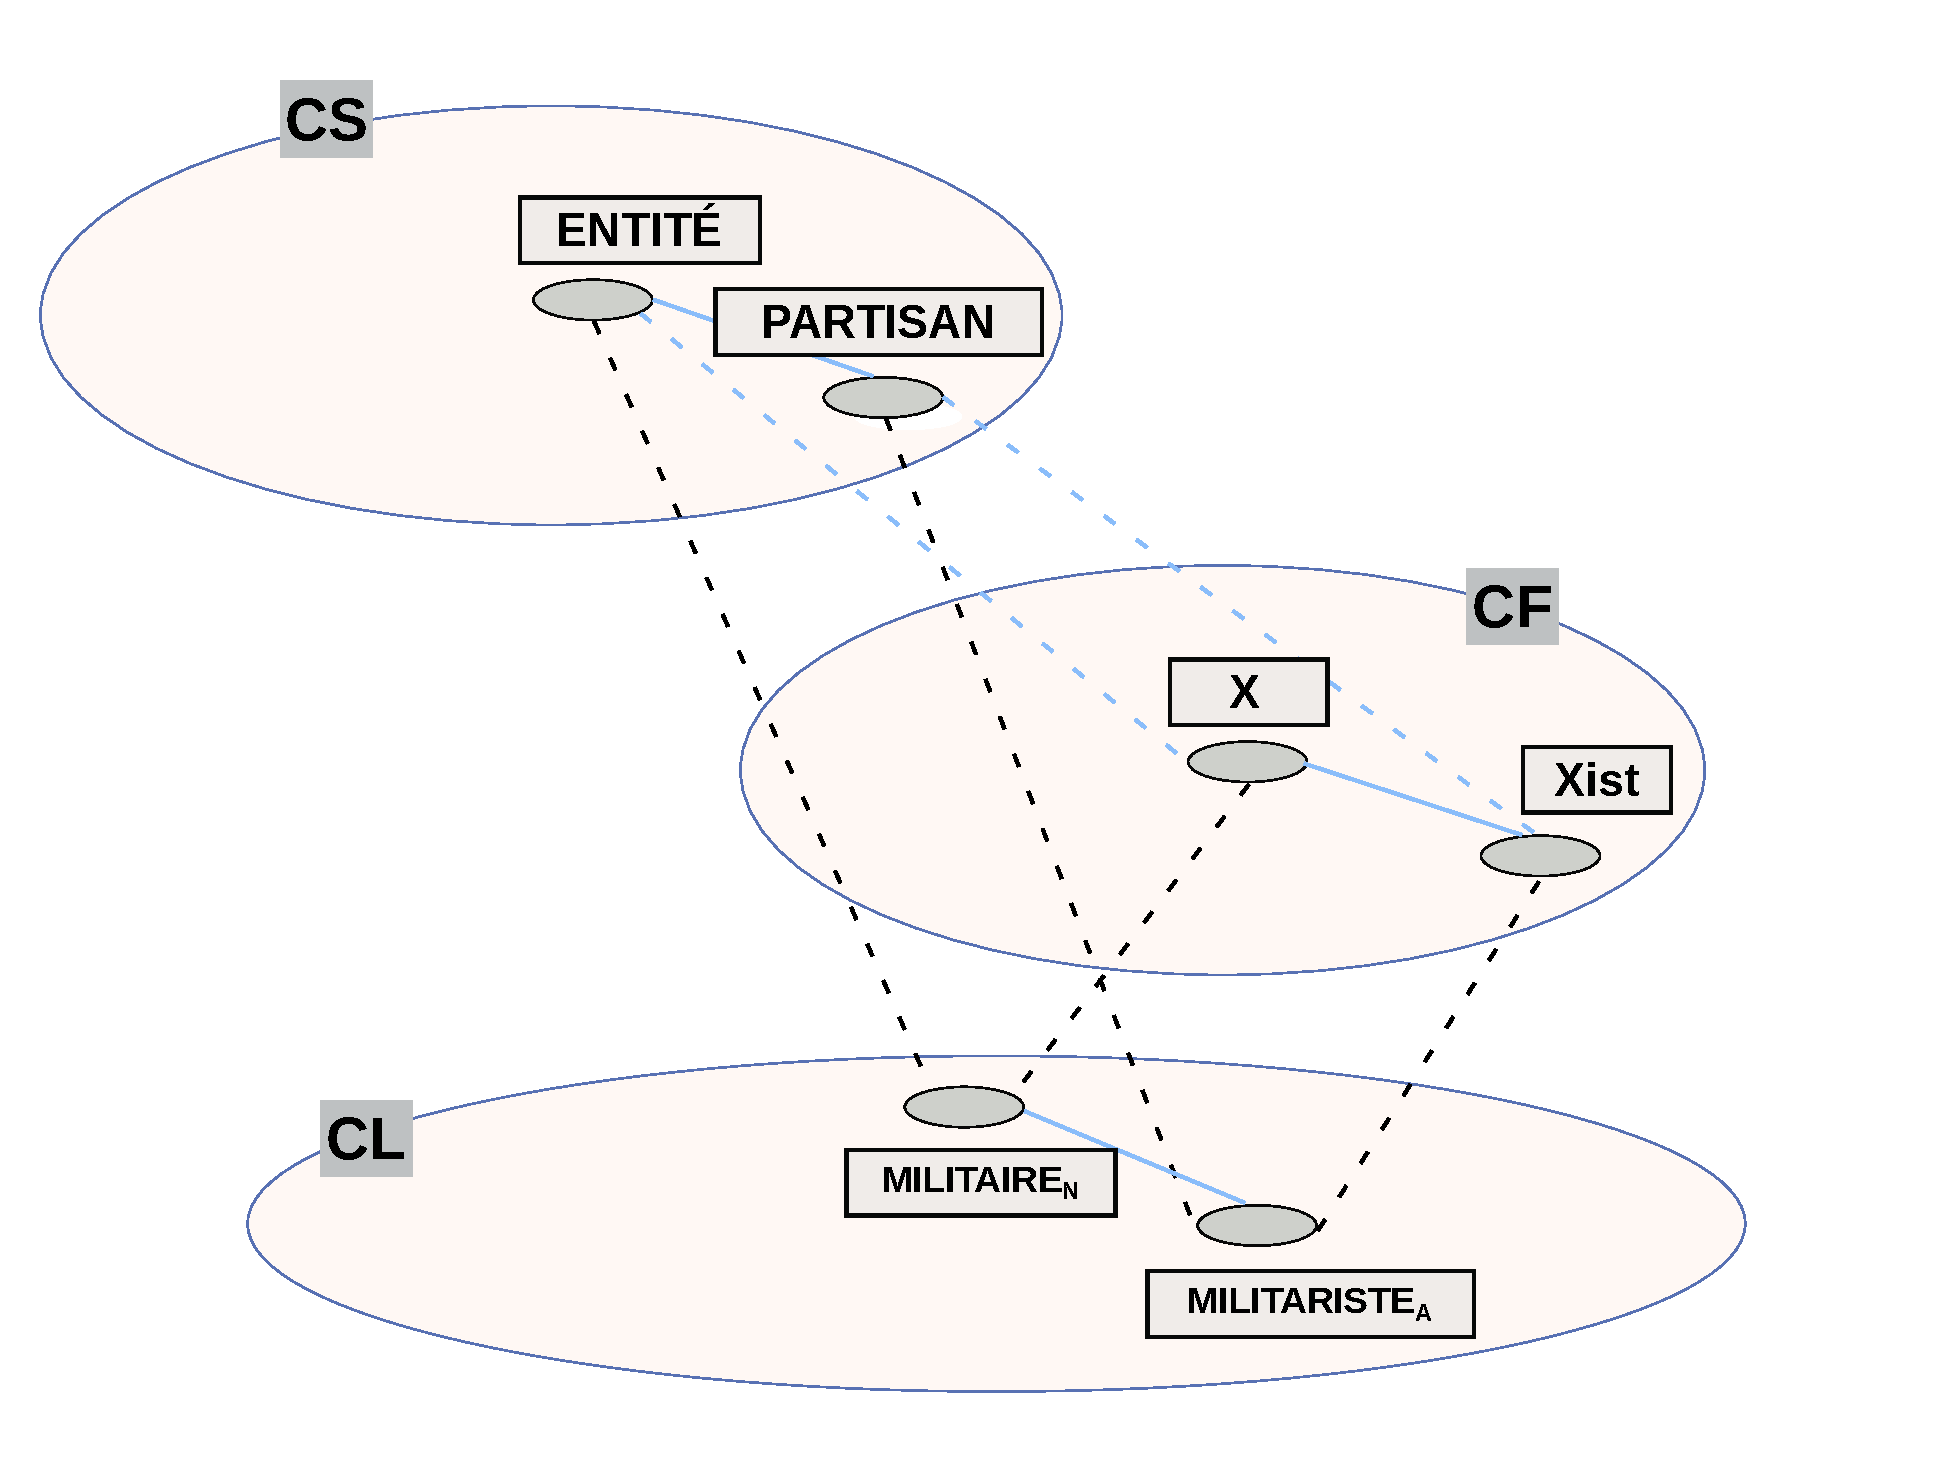
\includegraphics[width=0.8\linewidth]{figures/hathoutnamer-anti3.pdf}}
  \fbox{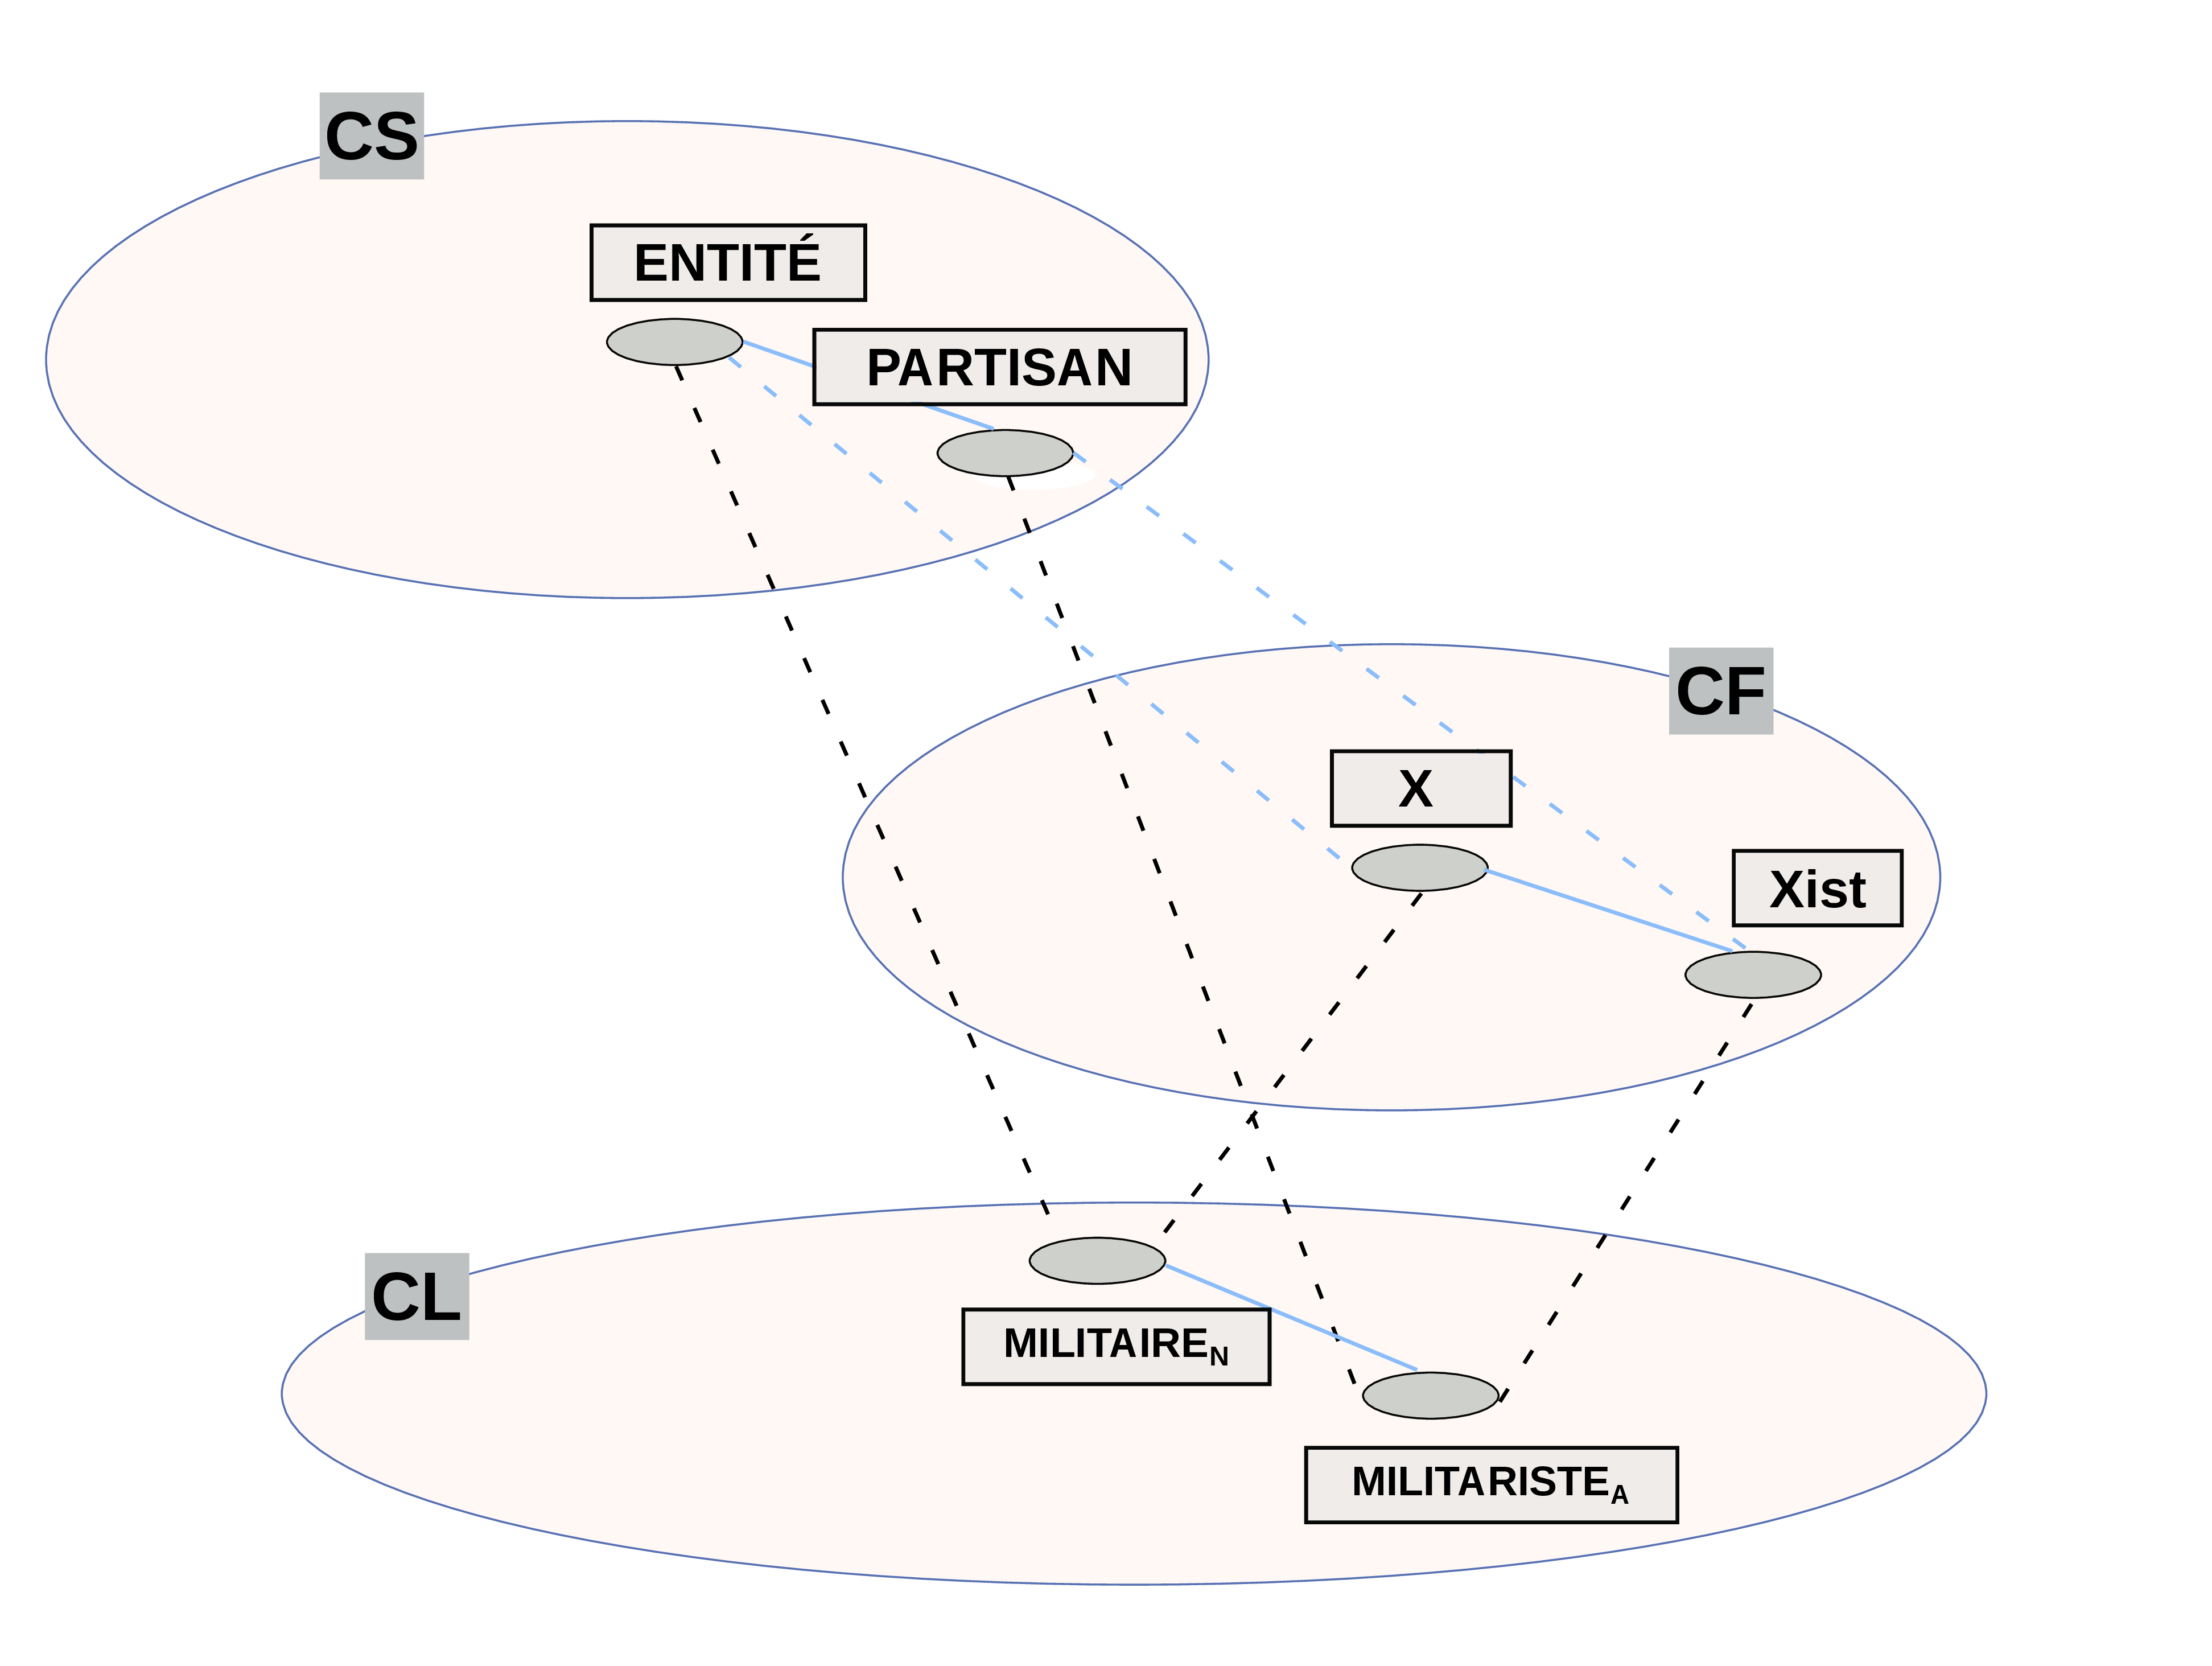
\includegraphics[width=0.8\linewidth]{figures/hathoutnamer-anti3.png}}
  \caption{Module régulier (\textsc{militariste}, \textsc{militaire})}
  \label{fig:antimilitariste3}
\end{figure}

En rassemblant les éléments d'analyse que nous venons de présenter, on voit que la forme et le sens de \textsc{antimilitariste} résultent d'une combinaison de facteurs qui interviennent de façon inégale~:
%
\begin{enumerate}
\item \textsc{antimilitariste} et \textsc{militaire} sont sémantiquement motivés l'un par l'autre (figure~\ref{fig:antimilitariste1})~;
\item \textsc{antimilitariste} et \textsc{militariste} sont formellement motivés l'un par l'autre (figure~\ref{fig:antimilitariste2})~;
\item \textsc{militariste} et \textsc{militaire} sont sémantiquement et formellement connectés (figure~\ref{fig:antimilitariste3}).
\end{enumerate}
%
Cette convergence de propriétés fait intervenir l'unification, au niveau du CF\is{ParaDis model!formal component}, du $X$ de la figure~\ref{fig:antimilitariste3} avec le $Y\textrm{ɛʁ}$  de la figure~\ref{fig:antimilitariste1}, ce qui conduit à la spécification (\ref{exe:yariste}b) de la relation formelle (\ref{exe:yariste}a) de la suffixation en /ist/\is{suffixation!in -\emph{iste}}. La variation /ɛʁ/-/ɑʁ/ 
 en (\ref{exe:yariste}b) est due à la proximité de la voyelle /ɛ/ 
  avec le /i/ 
 dans /ist/~:
%
\begin{exe}
\ex\label{exe:yariste}\begin{tabular}[t]{cccc}
a. & $X$ &	--- &	$X$iste\\
 & \rotatebox{90}{=} & & \rotatebox{90}{=}\\
b. & $Y$aire& 	--- &	$Y$ariste
\end{tabular}
\end{exe}

Le résultat, présenté dans la figure~\ref{fig:antimilitariste}, est un module\is{ParaDis model!module} dont les trois composants\is{ParaDis model!abstract component} sont entièrement interconnectés, avec un composant lexical\is{ParaDis model!lexical component} formant un graphe complet, et les composants sémantique\is{ParaDis model!semantic component} et formel\is{ParaDis model!formal component} constituant chacun un graphe connexe acyclique dont les sommets reliés sont différents. Comme on peut le voir, la figure~\ref{fig:antimilitariste} est une simple superposition des sous-modules des figures~\ref{fig:antimilitariste1}, \ref{fig:antimilitariste2} et \ref{fig:antimilitariste3}. La non-coïncidence  entre les trois composants abstraits\is{ParaDis model! abstract component} dans la figure~\ref{fig:antimilitariste} se manifeste dans la géométrie des composants du module\is{ParaDis model!module} complet de \textsc{antimilitariste}.  Elle contraste avec la géométrie régulière du module\is{ParaDis model!module} de (\textsc{vider}, \textsc{videur}, \textsc{vidage}) illustré par la figure~\ref{fig:module-regulier} dont la canonicité paradigmatique\is{paradigm!derivational paradigm}\is{canonicity!paradigmatic} se traduit par la coprésence de trois triangles isomorphes\is{ParaDis model!isomorphy between components}.
%
\begin{figure}
  \centering
%   \fbox{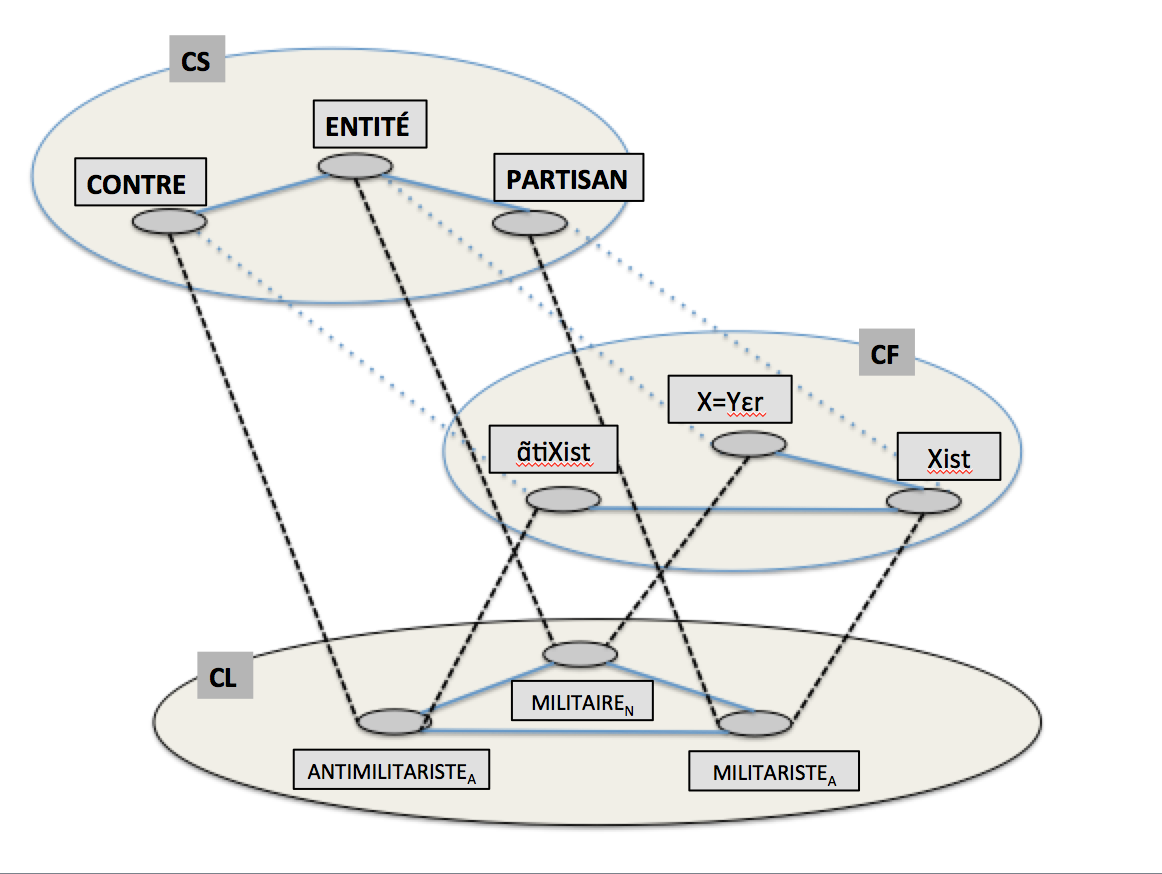
\includegraphics[width=0.8\linewidth]{figures/HatoutNamermodule-antimilitariste-new.png}}
%   \fbox{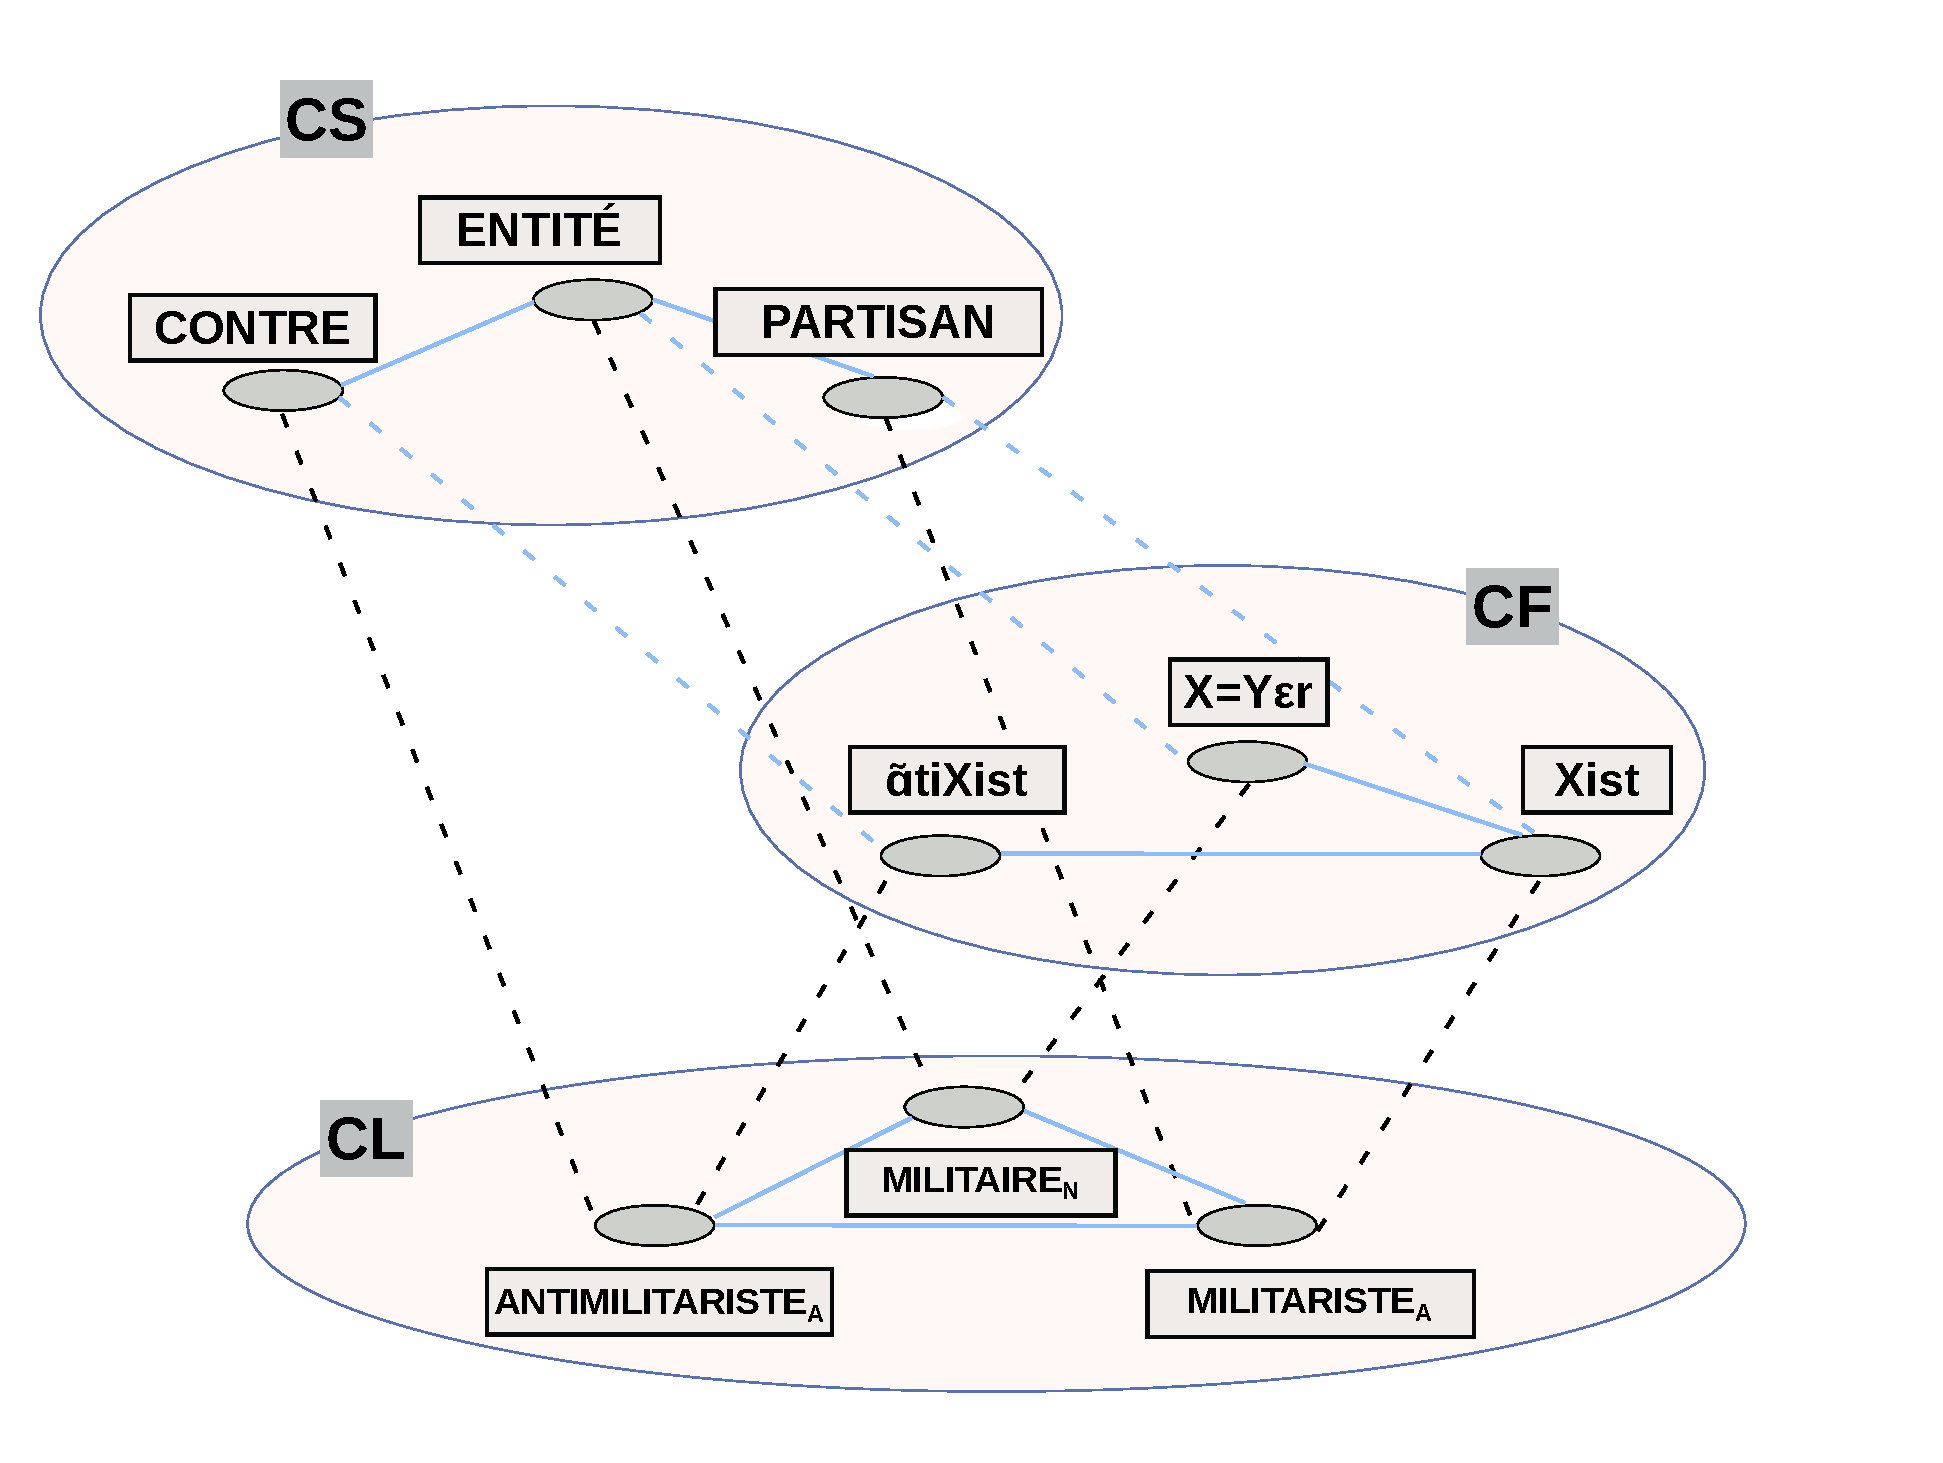
\includegraphics[width=0.8\linewidth]{figures/hathoutnamer-antinew.pdf}}
  \fbox{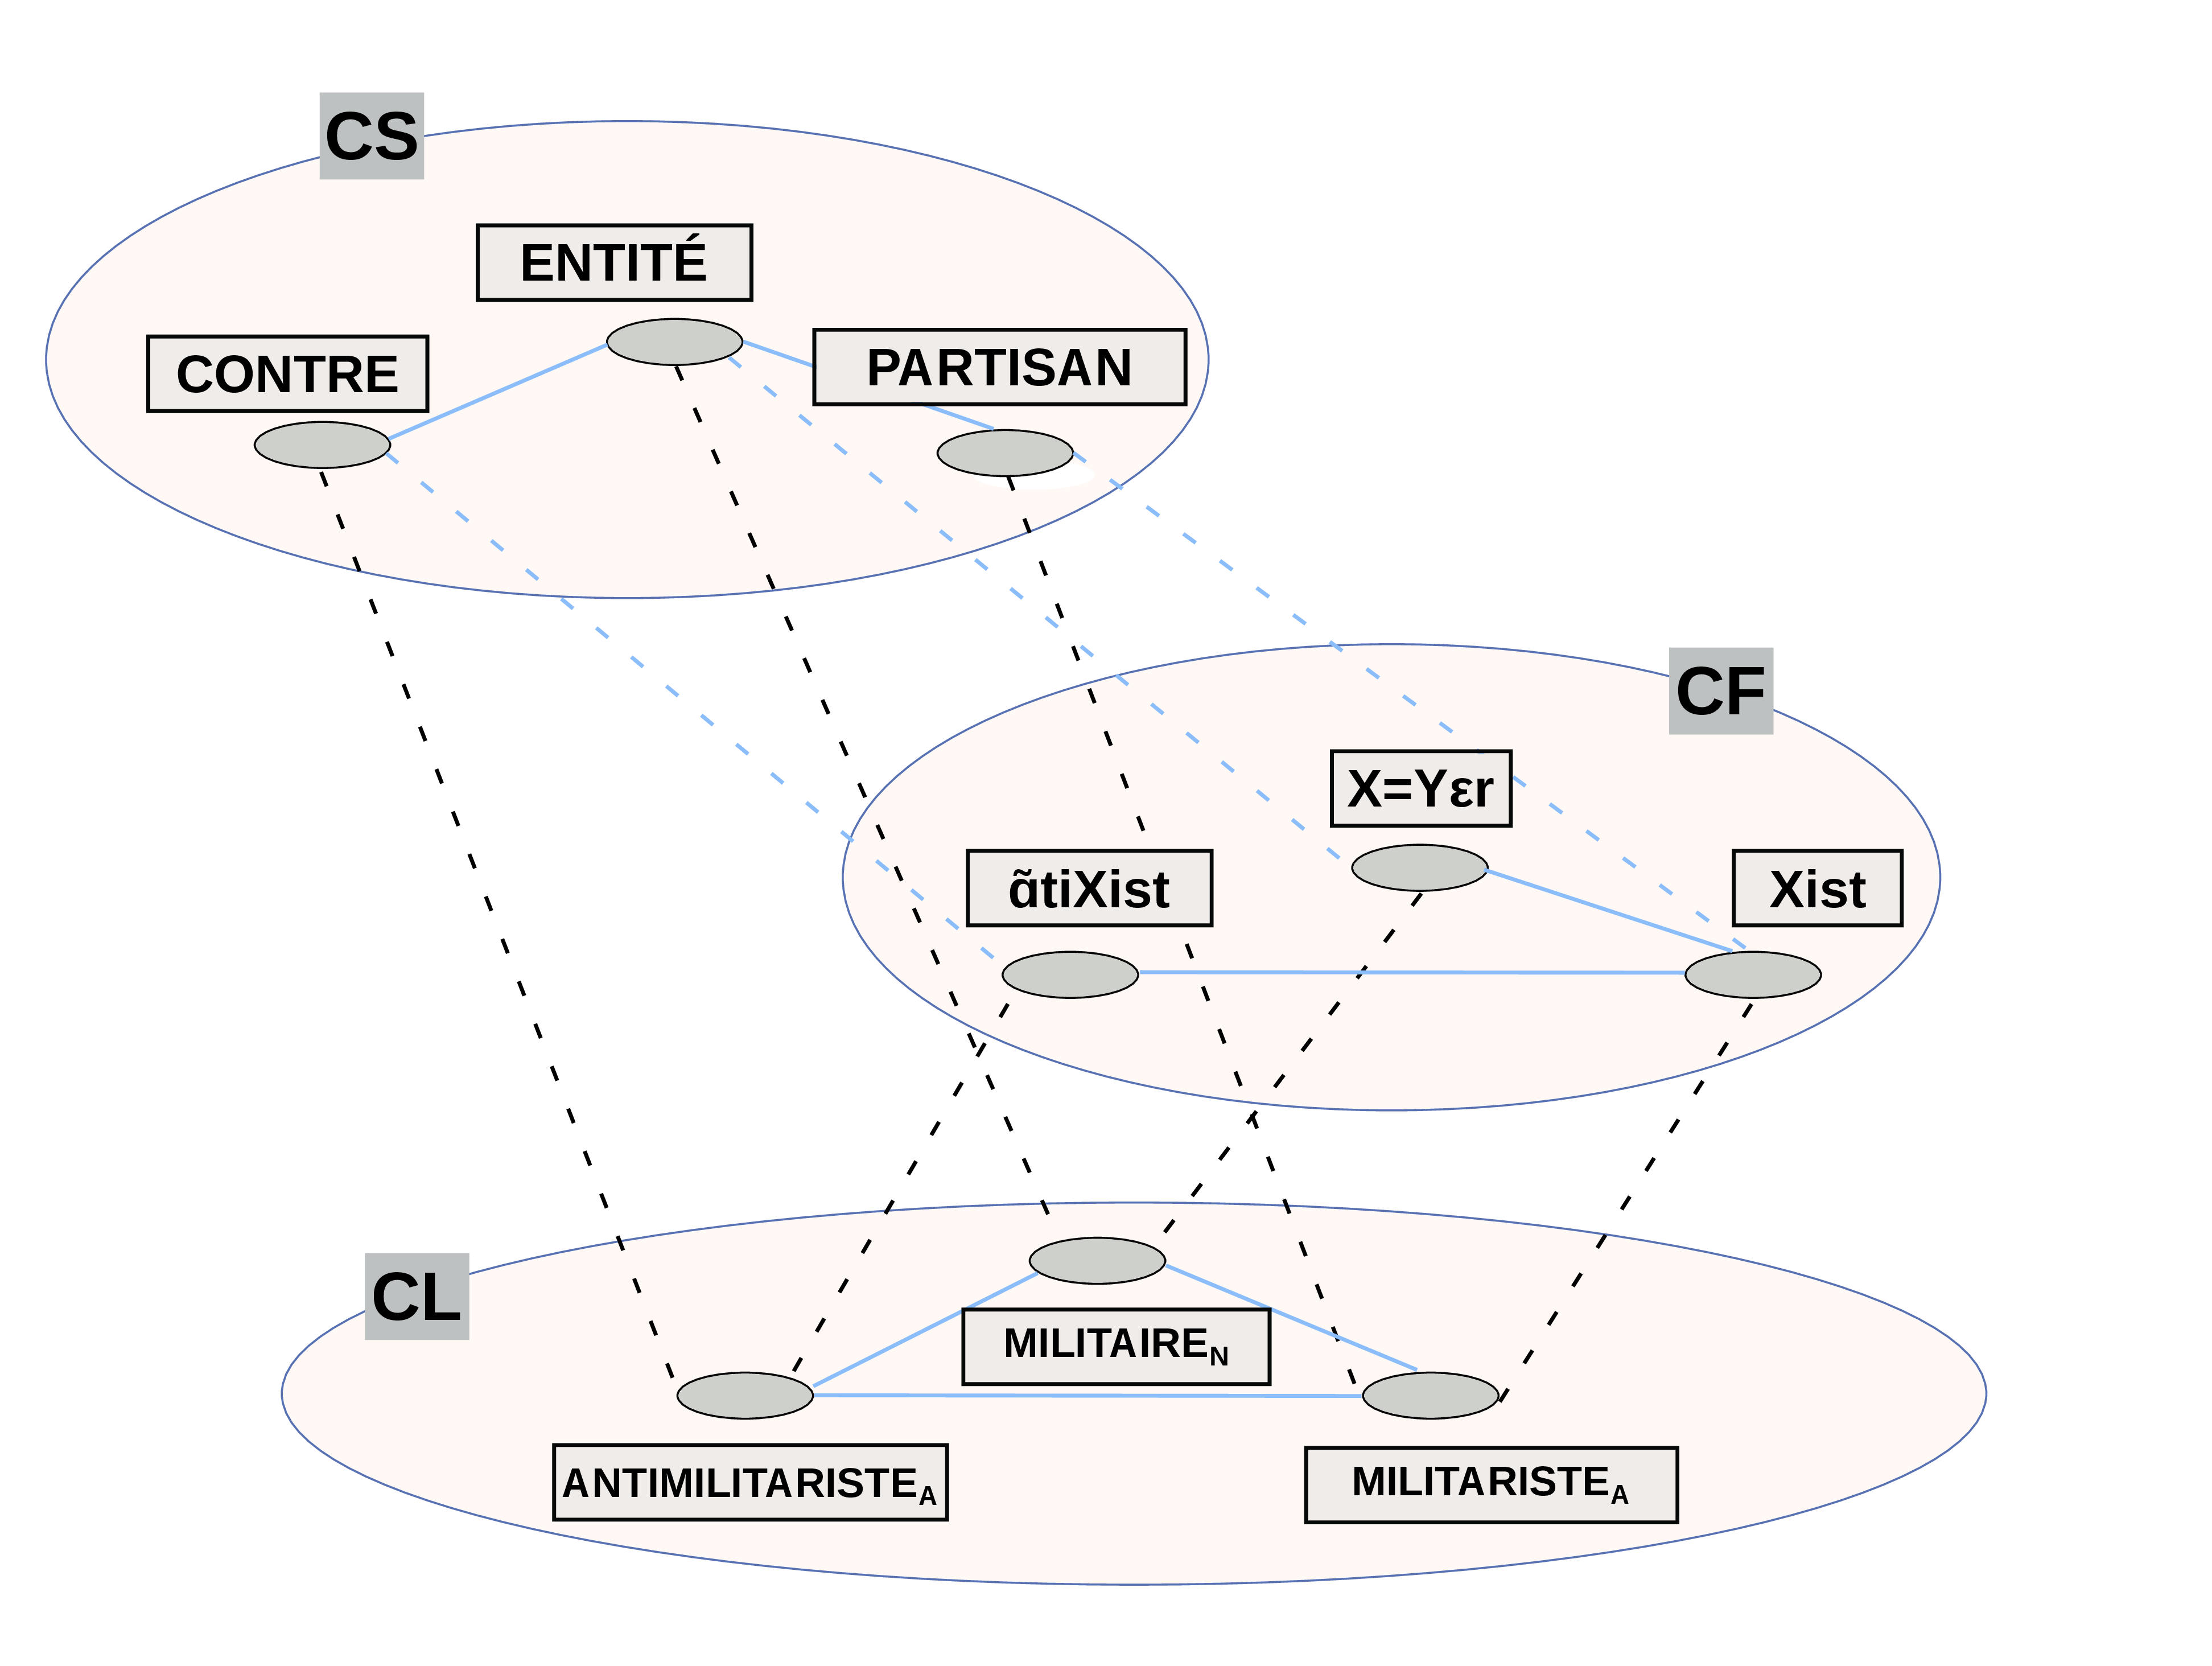
\includegraphics[width=0.8\linewidth]{figures/hathoutnamer-antinew.png}}
  \caption{Module décrivant à l'analyse de \textsc{antimilitariste}}
  \label{fig:antimilitariste}
\end{figure}

\is{ParaDis model|)}
\subsection{Pour récapituler}
\label{sec:pour-recapituler}
Le modèle \paradis{}\is{ParaDis model} résulte d'un triple héritage~: il s'inspire des \emph{Patrons Cumulatifs}\is{Cumulative Pattern} de Bochner qui essentiellement décrivent les composantes formelles et catégorielles de la dérivation morphologique\is{derivation}.  \paradis{}\is{ParaDis model} les étend à la dimension sémantique des paradigmes\is{paradigm!derivational paradigm} et tire parti du fonctionnement indépendant et simultané des composants formel\is{ParaDis model!formal component}, catégoriel\is{ParaDis model!categorial component} et sémantique\is{ParaDis model!semantic component} des RCL\is{lexeme formation rule} et de la nature tri-dimensionnelle des lexèmes\is{lexeme!tridimensional structure} sur lesquels elles s'appliquent.  Enfin,  \paradis{}\is{ParaDis model} adopte, dans le but de la formaliser, l'organisation en réseau de la morphologie\is{morphology!Network Morphology} constructionnelle initiée par l'axe DUMAL qu'il complète en les articulant avec les structures paradigmatiques de famille\is{derivation!derivational family} et de série dérivationnelles\is{derivation!derivational series}.

De cette manière, la distribution et le traitement des informations morphologiques de  \paradis{}\is{ParaDis model} servant à réaliser l'analyse des constructions morphologiques, et notamment des dérivés parasynthétiques, s'effectue sur trois plans~:
%
\begin{itemize}
\item[---] suivant les trois dimensions classiques du lexème\is{lexeme!tridimensional structure}~;
\item[---] auprès des membres de la famille dérivationnelle\is{derivation!derivational family} du dérivé que l'on souhaite décrire~;
\item[---] à travers les relations entre les séries dérivationnelles\is{derivation!derivational series} dans lesquelles s'insèrent les lexèmes\is{lexeme} de cette famille.
\end{itemize}

Avec cette organisation multi-niveaux \paradis{}\is{ParaDis model} peut appréhender la construction morphologique aussi bien sous forme de relations binaires, que du point de vue de modules\is{ParaDis model!module} plus complexes instanciant les réseaux de motivation\is{derivation!motivation} paradigmatiques\is{paradigm!derivational paradigm} des dérivés morphologiques~; l'organisation proposée permet de traiter de manière uniforme tous les types de dérivés, quel que soit leur éloignement vis-à-vis de la situation idéale de transparence formelle et sémantique.  Relativement aux modèles qui l'on précédé, \paradis{}\is{ParaDis model} peut donc traiter les apparentes anomalies constructionnelles que manifestent les dérivés parasynthétiques, sans recourir à des artéfacts analytiques~: les mécanismes qui servent à les analyser sont strictement identiques à ceux qui permettent d'analyser les dérivations canoniques\is{canonicity!derivational}.  Les relations formelles et sémantiques asynchrones qui induisent leur écart relativement à la situation canonique sont envisagées de manière disjointe, se traduisant, dans le cas de la parasynthèse, par une autonomisation de la motivation du préfixe\is{prefixation} et de la séquence suffixale\is{suffixation!suffixal sequence}.  La disponibilité de la famille\is{derivation!derivational family} du dérivé parasynthétique, distribuée dans les différents composants\is{ParaDis model!four representation levels}, et sa structure en réseaux permettent de calculer la forme appropriée de la séquence finale.

\is{parasynthesis|)}
\il{French|)}

{\sloppy
    \printbibliography[heading=subbibliography,notkeyword=this]
}

\end{document}
